\chapter{Implementierung} \label{cha:Implementierung}

In diesem Kapitel soll das zuvor vorgestellte Verfahren implementiert werden. Zuerst wird die experimentelle Umgebung auf dem Matlab vorgestellt. Anschließend die Implementierung der beiden vorherigen Methoden, welche die verarbeiteten Daten jeden Schrittes und dessen Demonstration der Endergebnisse enthalten. Schließlich läuft die Implementierung des Detektionsverfahrens auf einer Smartphone-\gls{gpu}.

\section{Experimentelle Umgebung}

Hier wird die Experimentelle Umgebung auf dem Matlab erläutert. Das Google Pixel wird hier verwendet, um die Bilder aufzunehmen. Dessen Parameter sind in der Tabelle \ref{tbl:Parameter der Kameras im Vergleich} verfügbar. Die Anwendungssoftware $ ``VLCReceiver" $ wird mit einem automatischen Einstellungsmodus benutzt. Entsprechend dem möglichen Einsatzbereich des David-Systems wurden im Experiment Bildschirme verschiedener Größen und Umgebungen ausgewählt. Die in dem Experiment verwendeten Bildschirme sind in der Tabelle \ref{tbl:Verwendeter Bildschirm} zu sehen. Die aufgenommenen Bilder werden auf der PC-Seite mit Matlab 2017b unter der Lizenz der TU Dortmund verarbeitet.

\begin{table}[htb]
	\captionabove{Verwendete Bildschirme}
	\label{tbl:Verwendeter Bildschirm}
	\footnotesize
	\centering
	\rowcolors{2}{white}{gray!25}	%TUgreen!25
	%\begin{tabular}{|p{3cm}|p{2cm}|p{2cm}|p{2cm}|p{2cm}|p{2cm}|}	%p{}m{}b{}clr
	\begin{tabular}{|c|c|c|c|c|c|}
	\toprule
	\textbf{Hersteller} & \textbf{Model} & \textbf{Beleuchtung} & \textbf{Auflösung} & \textbf{Größe}	& \textbf{Frequenz}\\
	\midrule
	Lenovo Notebook & T440P & LED & $ 1920 \times 1280$ & 14'' & 60 \\
	Samsung 	  & SMB2440MH   & LED & $ 1920 \times 1280$ & 24'' & 60 \\
	Ausu  		  & VG248   & LCD & $ 1920 \times 1280$ & 24'' & 60 \\
	LG  		  & 55EF950V & OLED & $ 2160 \times 3840$ & 55'' & 120 \\
	
	\bottomrule
	\end{tabular}
\end{table} 

\section{Implementierung vom ersten Verfahren}
Im Implementierungsprozess der Methode 1, stammt das Bild aus einer Reihe von acht Bildern, die mit einer Smartphonekamera aus die Hand aufgenommen wurden. Entsprechend den Eigenschaften der Bildregistrierung in dieser Arbeit sind die von der handgehaltenen Kamera aufgenommenen Objekte alles statische Videos. Dies bedeutet, dass sich der Inhalt des Videos nicht ändert. Im tatsächlichen Betrieb entspricht es z.B. einer statischen elektronischen Werbetafel. Die Modulationsamplitude wird auf 6 gesetzt, der Daten Datenblock mit $ 4 \times 4 Pixel$ und die QR Muster Größe als $ 72 \times 72 Pixel$ initialisiert.

Aufgrund von Handschütteln während der Aufnahme entsteht eine leichte Verschiebung zwischen den Bildern. Um diesen Auswirkung zu verdeutlichen, wird das erste Bild und das achte Bild in Abbildung \ref{fig:vorregistration} verglichen. 
%Die durchschnittliche Entfernung der entsprechenden Pixel zwischen den zwei Bildern beträgt ca.2 Pixel. 
Abbildung \ref{fig:nachregis} zeigt das Bild nach der Bildregistration. Wie zu sehen ist, ist der Abstand komprimiert worden. %Die durchschnittliche Entfernung hier beträgt ca. 0.45 Pixel.
 
\begin{figure}[H]
\centering 
\begin{minipage}[b]{0.49\textwidth} 
\centering 
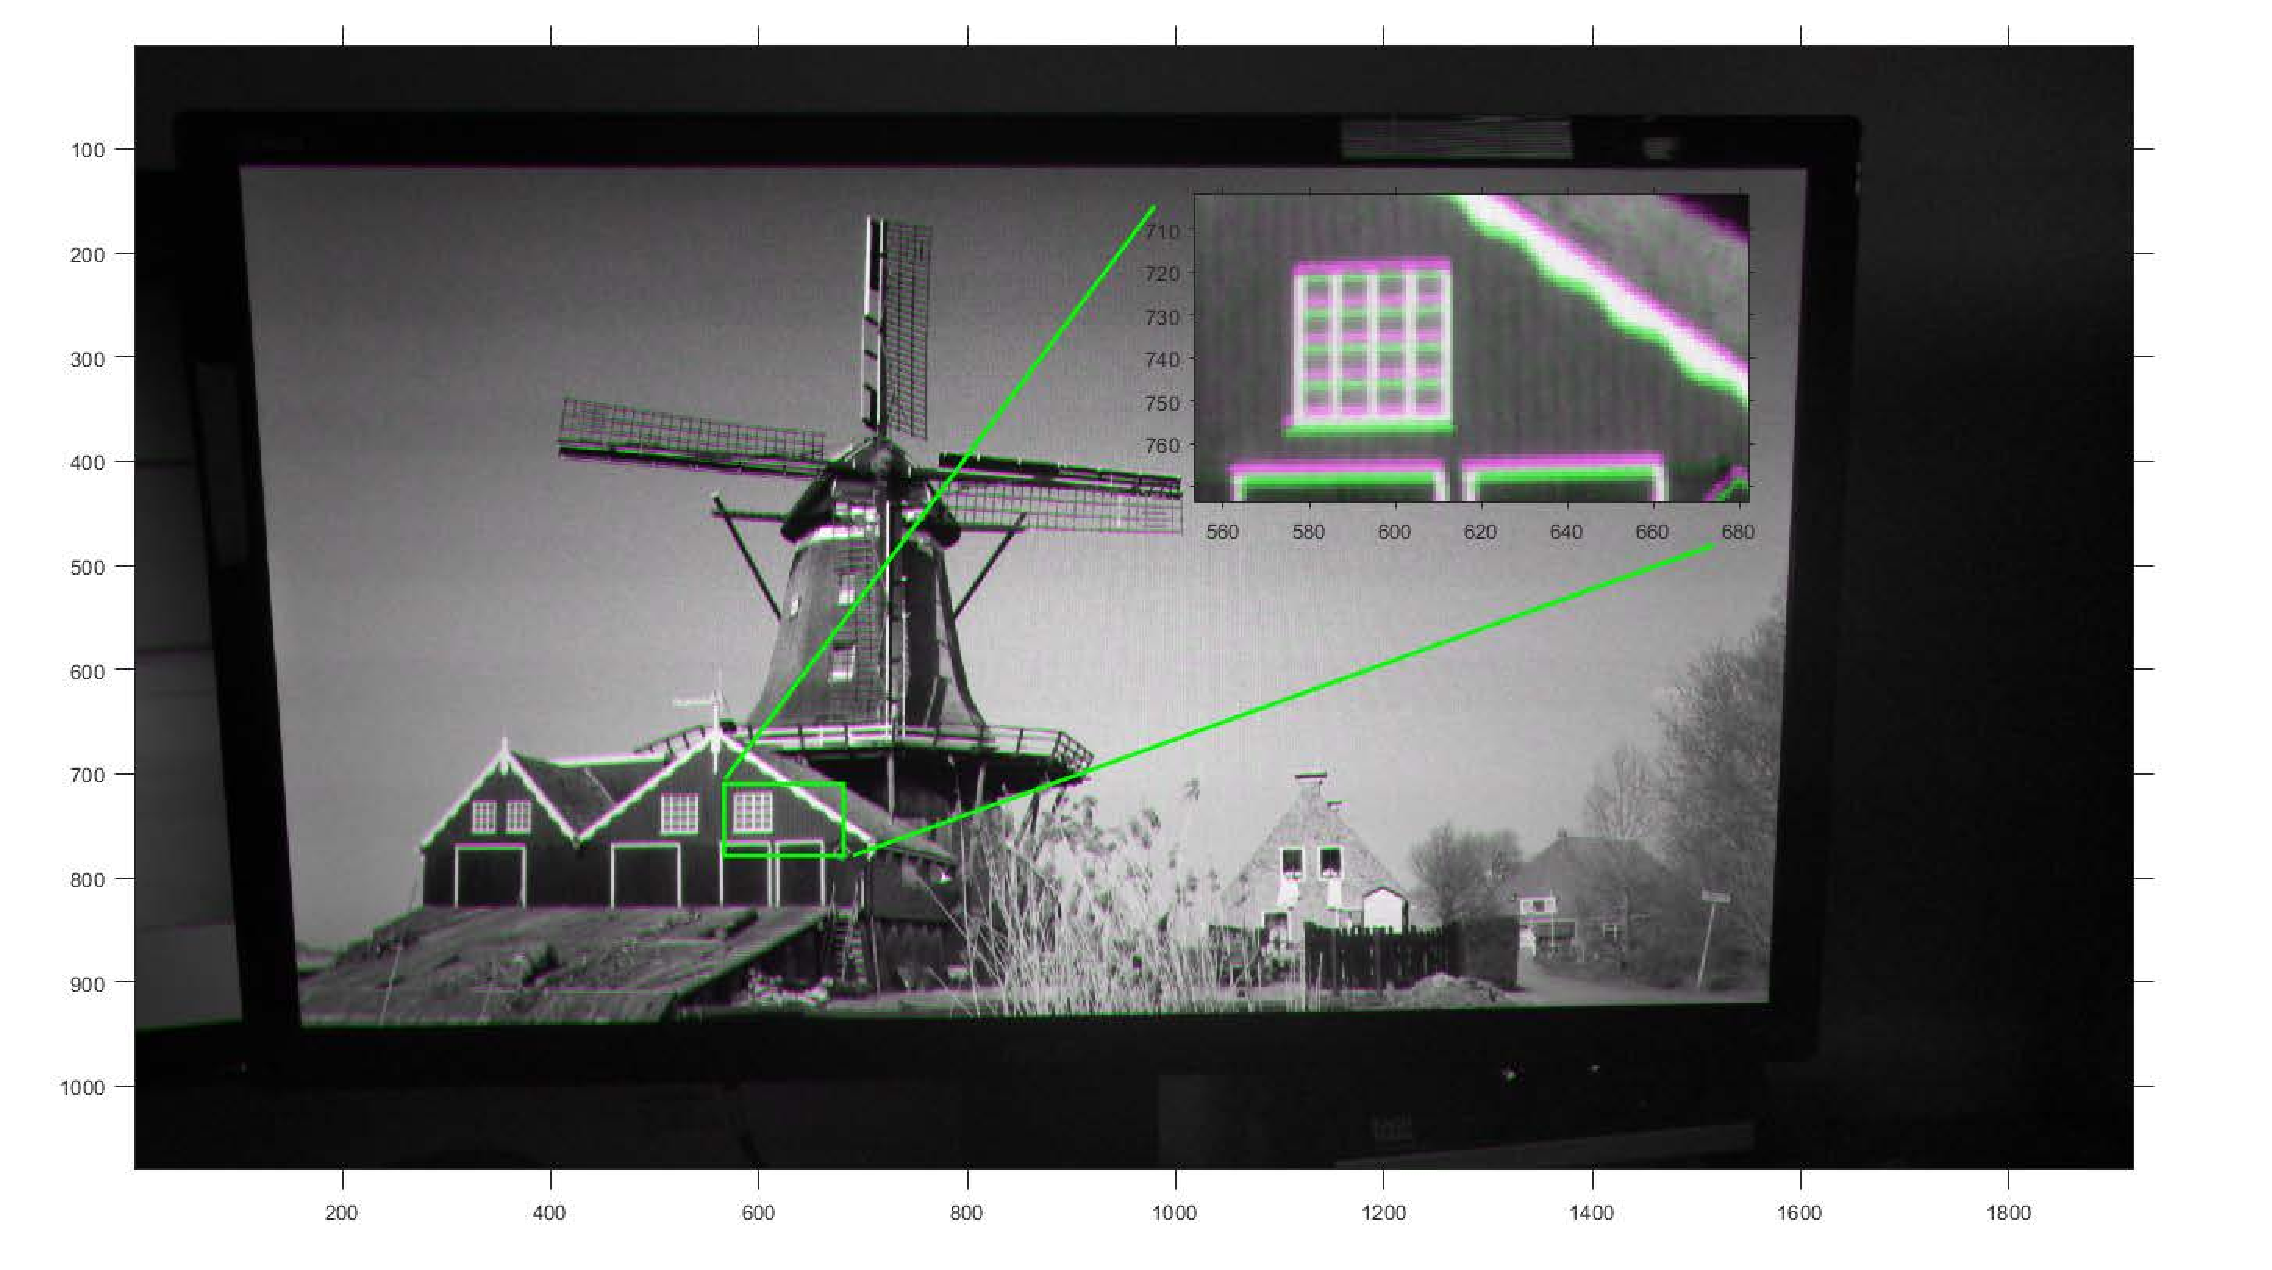
\includegraphics[width=1.0\textwidth]{images/5_Implementirung/vorregistration.pdf} 
\caption{Bilder vor Bildregistrierung}
\label{fig:vorregistration}
\end{minipage}
\begin{minipage}[b]{0.49\textwidth} 
\centering 
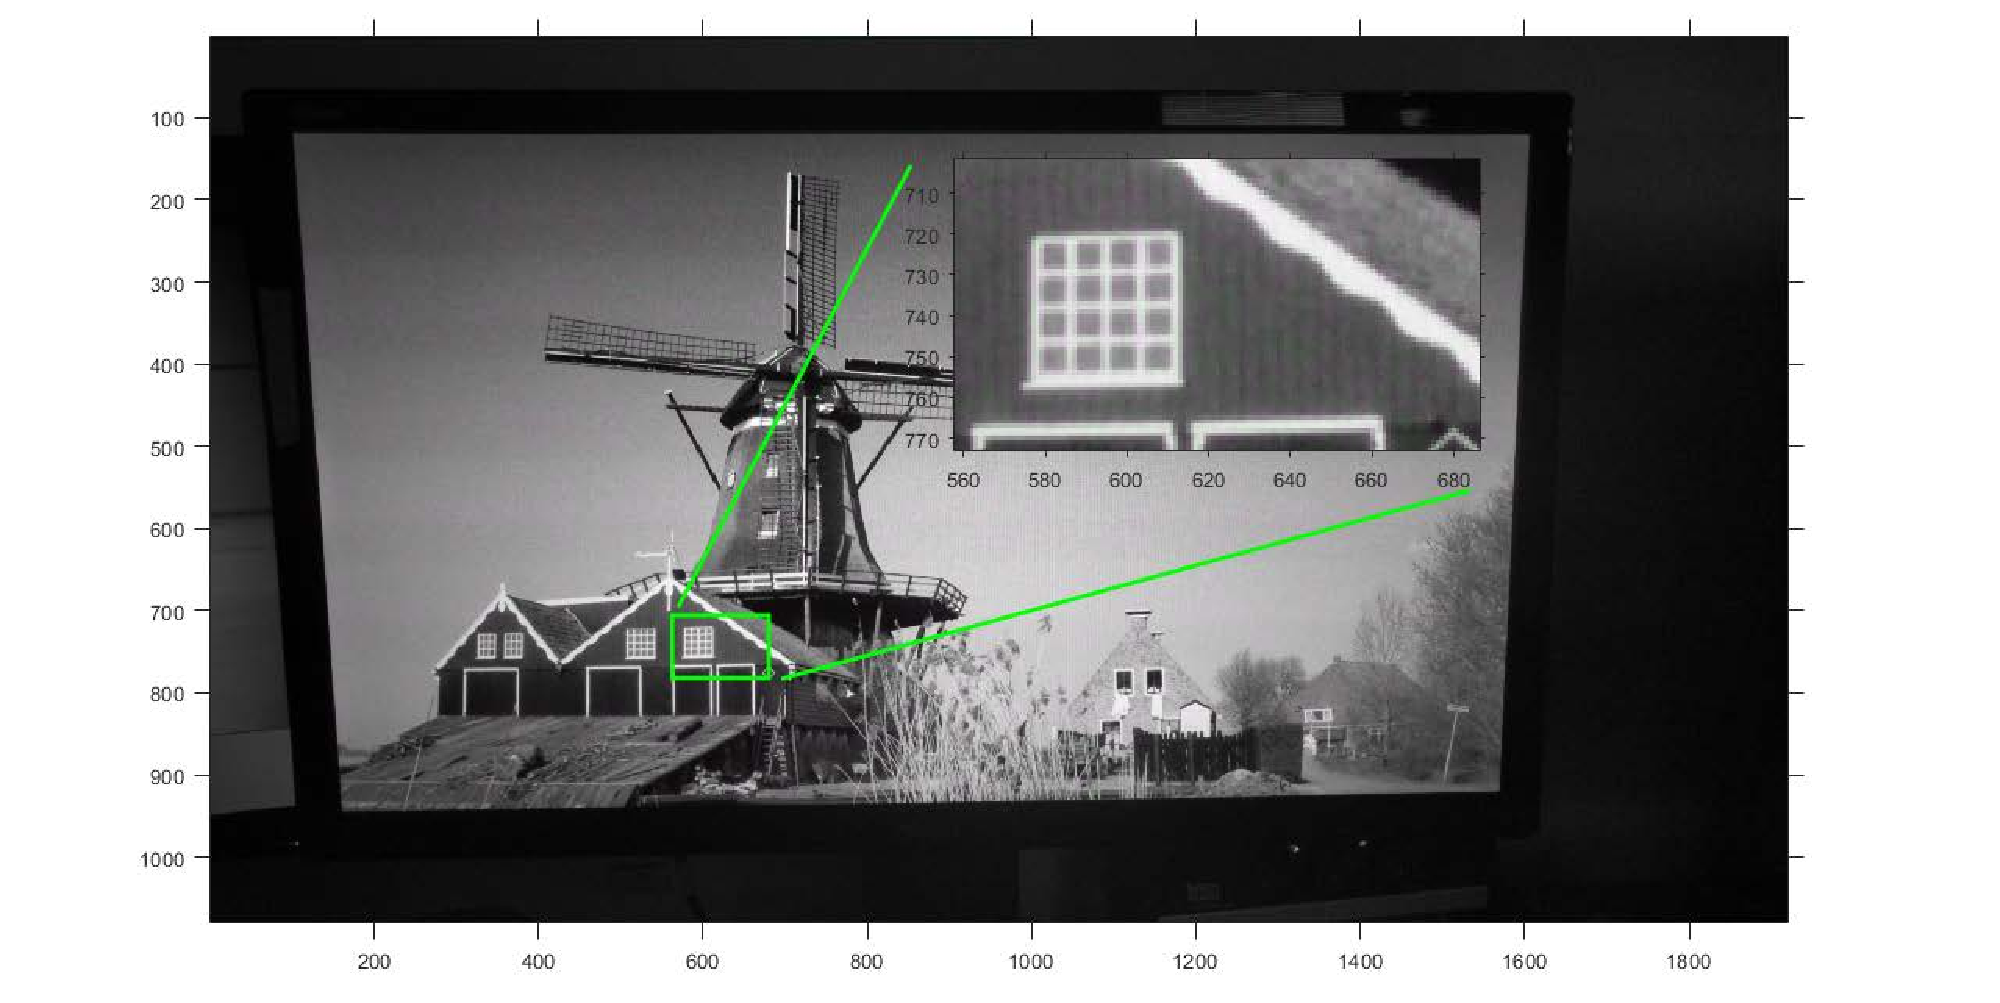
\includegraphics[width=1.1\textwidth]{images/5_Implementirung/nachregis.pdf}
\caption{Bilder nach Bildregistrierung}
\label{fig:nachregis}
\end{minipage}
\end{figure}
 
Aufgrund der Bildwiederholfrequenz werden die QR Muster in den Differenzbildern, wie in Tabelle \ref{tbl:differenzbildformel} zu sehen ist, einige unerwartete Effekte aufweisen. Um diese zu neutralisieren, wird eine Absolutwertoperation durchgeführt. Danach werden hier 3 Differenzbilder welche die größte ``Energie" beinhalten, überlagert um ein neues zu detektierende Bild entstehen. Das Ergebnis ist in Abbildung \ref{fig:nachdiff} zu sehen. 

%\begin{figure}[htbp]
%\centerings
%\subfigure[pic1.]{
%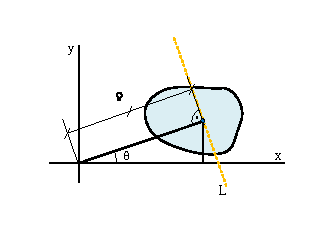
\includegraphics[keepaspectratio,width=0.45\textwidth]{images/5_Implementirung/1.eps}
%%\caption{fig1}
%}
%\quad
%\subfigure[pic2.]{
%\includegraphics[keepaspectratio,width=0.45\textwidth]{images/5_Implementirung/22.eps}
%}
%\quad
%\subfigure[pic3.]{
%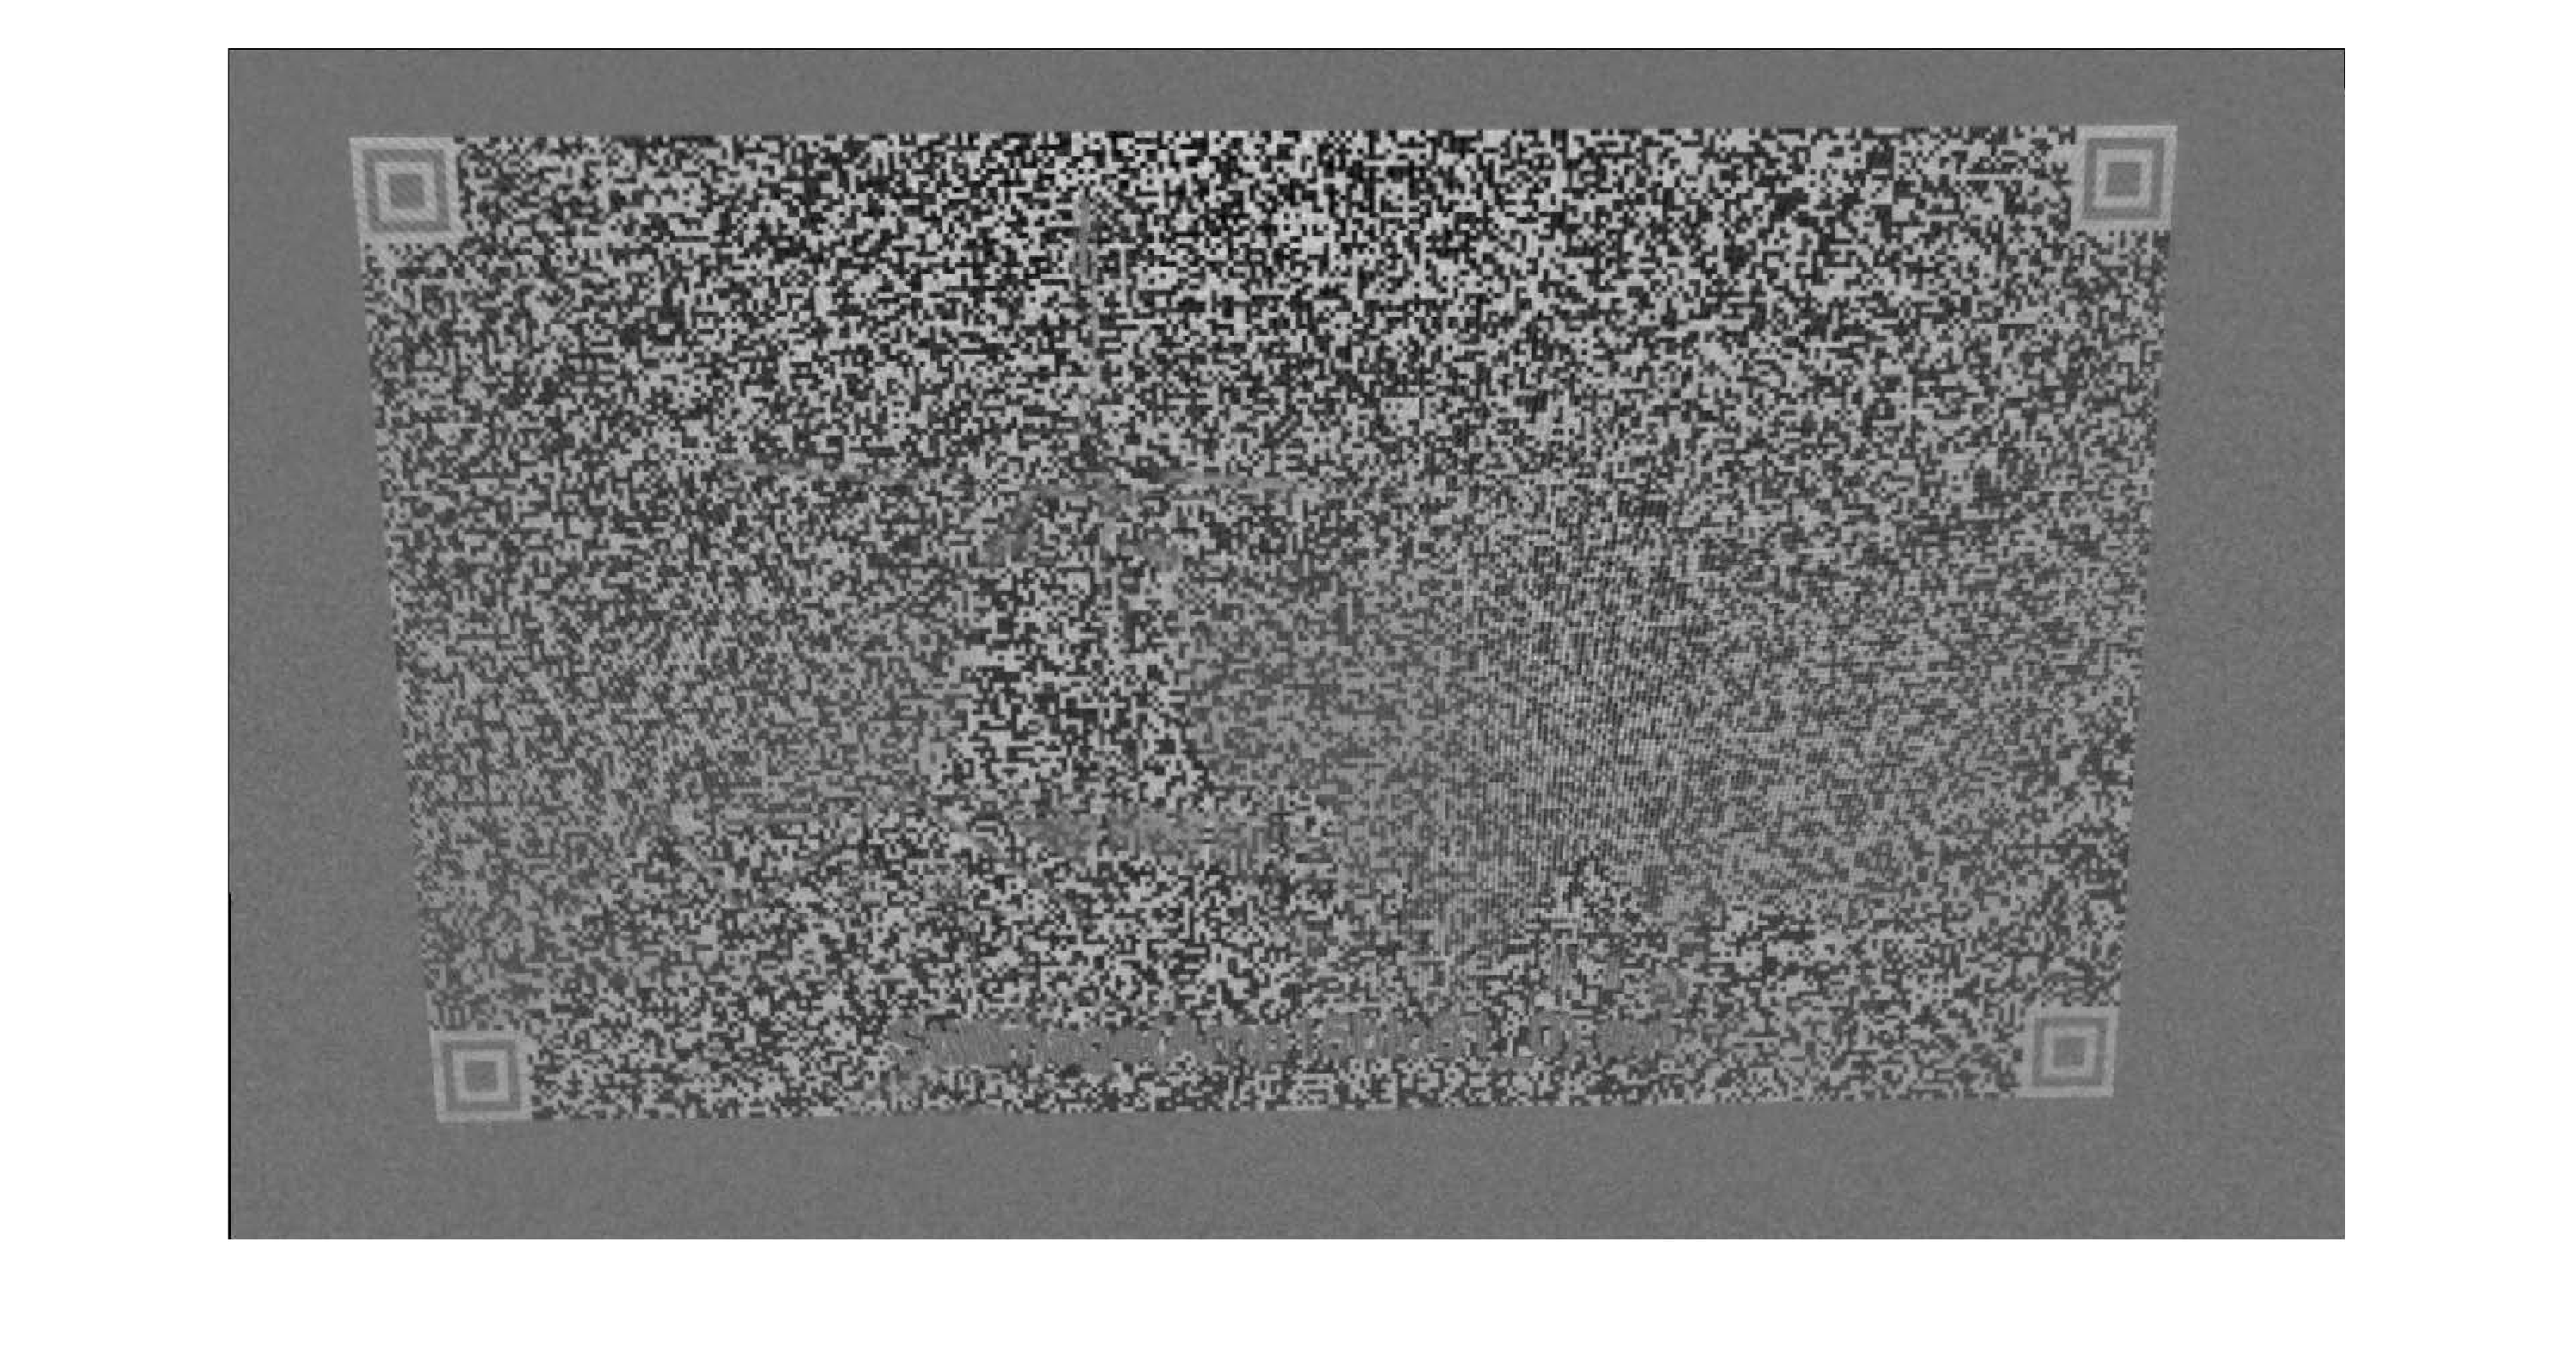
\includegraphics[keepaspectratio,width=0.49\textwidth]{images/3_Ersteverfahren/Differenzbild/0schwarz.pdf}
%}
%\quad
%\subfigure[pic4.]{
%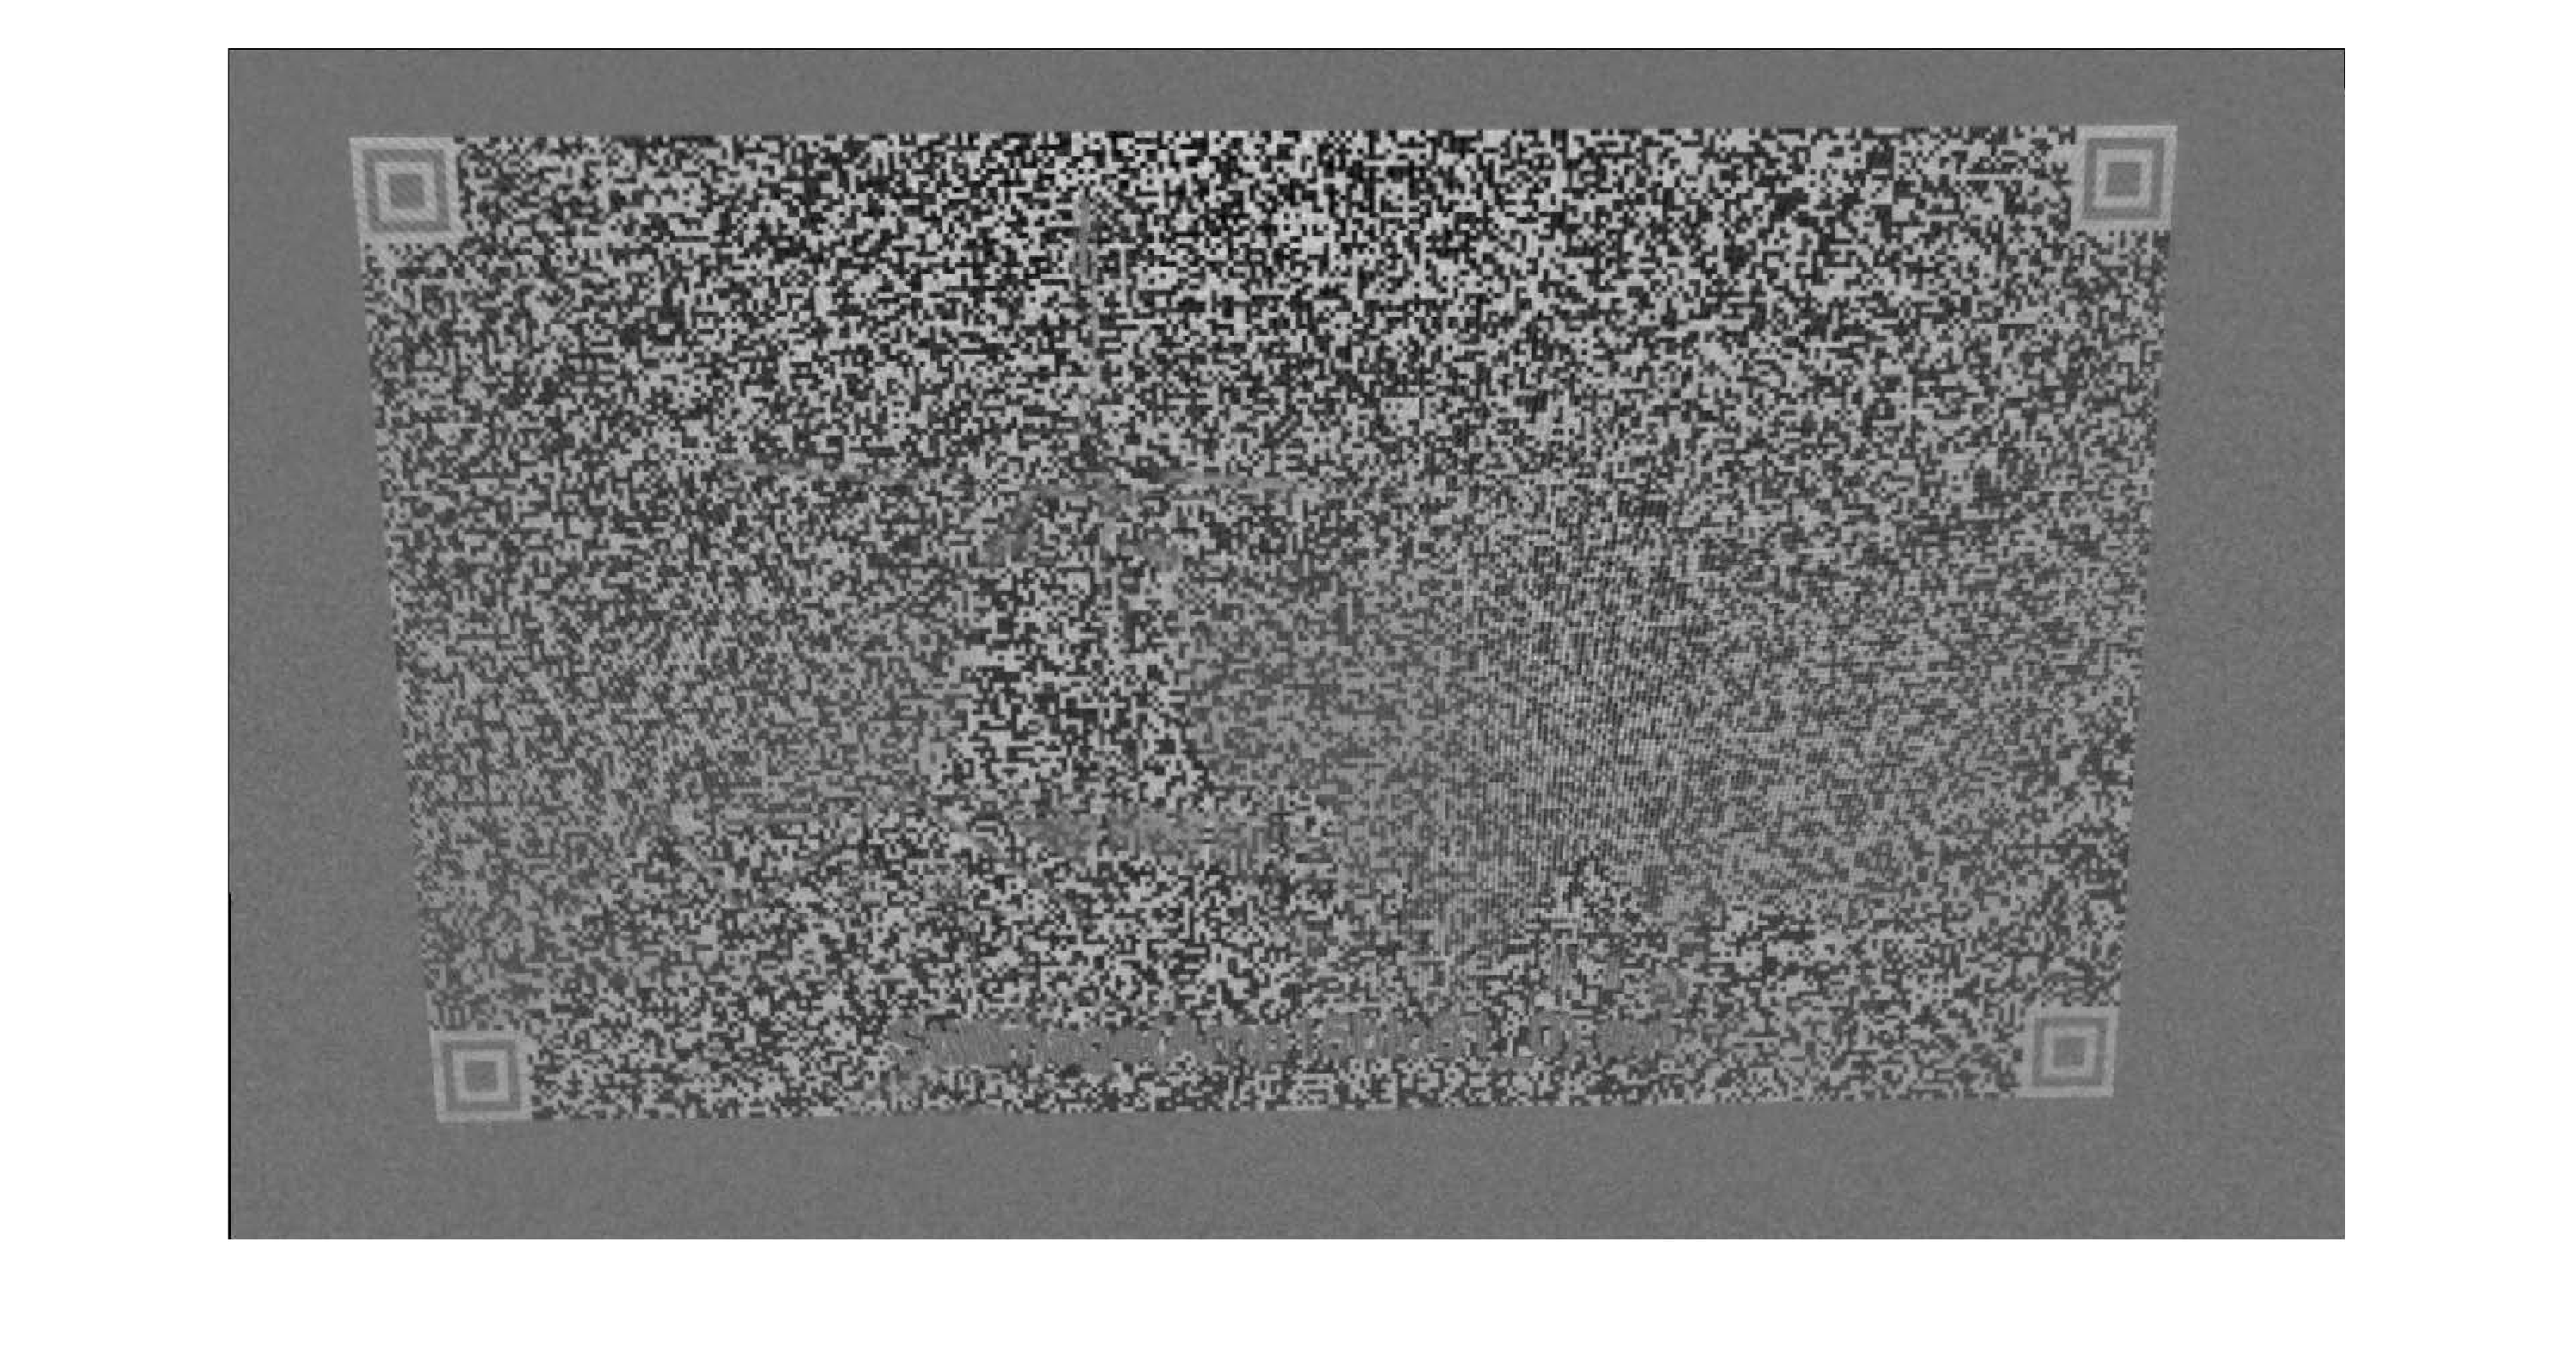
\includegraphics[keepaspectratio,width=0.45\textwidth]{images/3_Ersteverfahren/Differenzbild/0schwarz.pdf}
%}
%\quad
%\subfigure[pic5.]{
%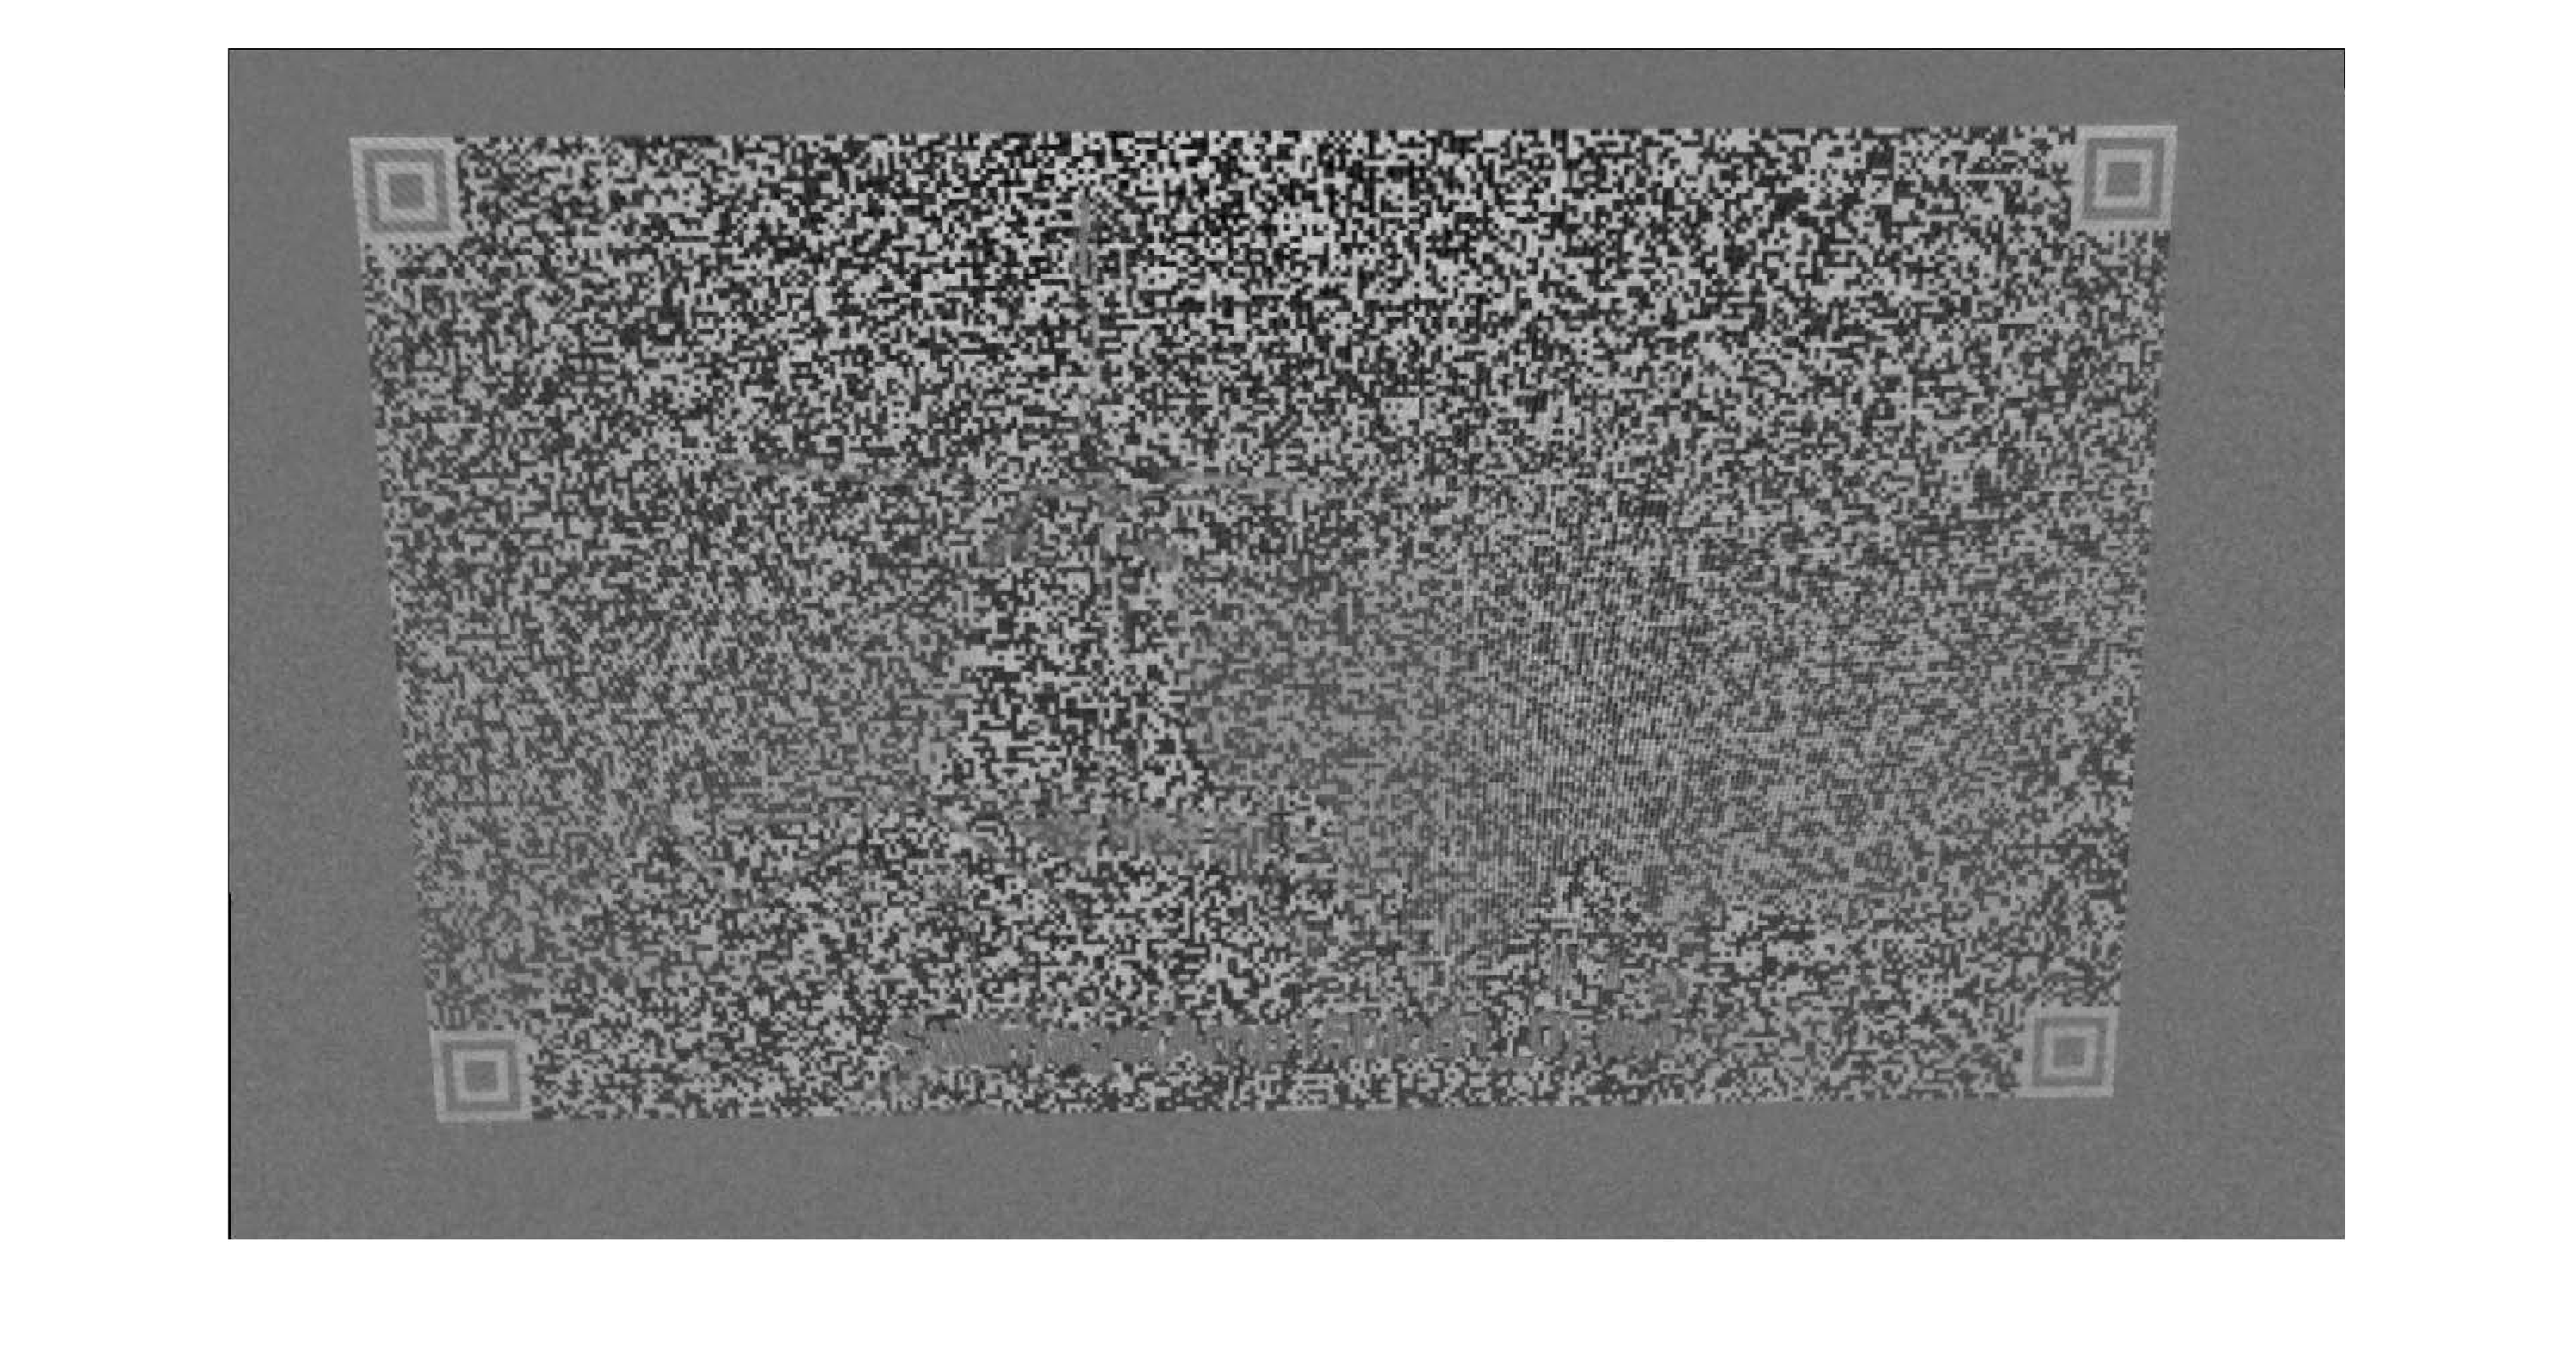
\includegraphics[keepaspectratio,width=0.45\textwidth]{images/3_Ersteverfahren/Differenzbild/0schwarz.pdf}
%}
%\quad
%\subfigure[pic6.]{
%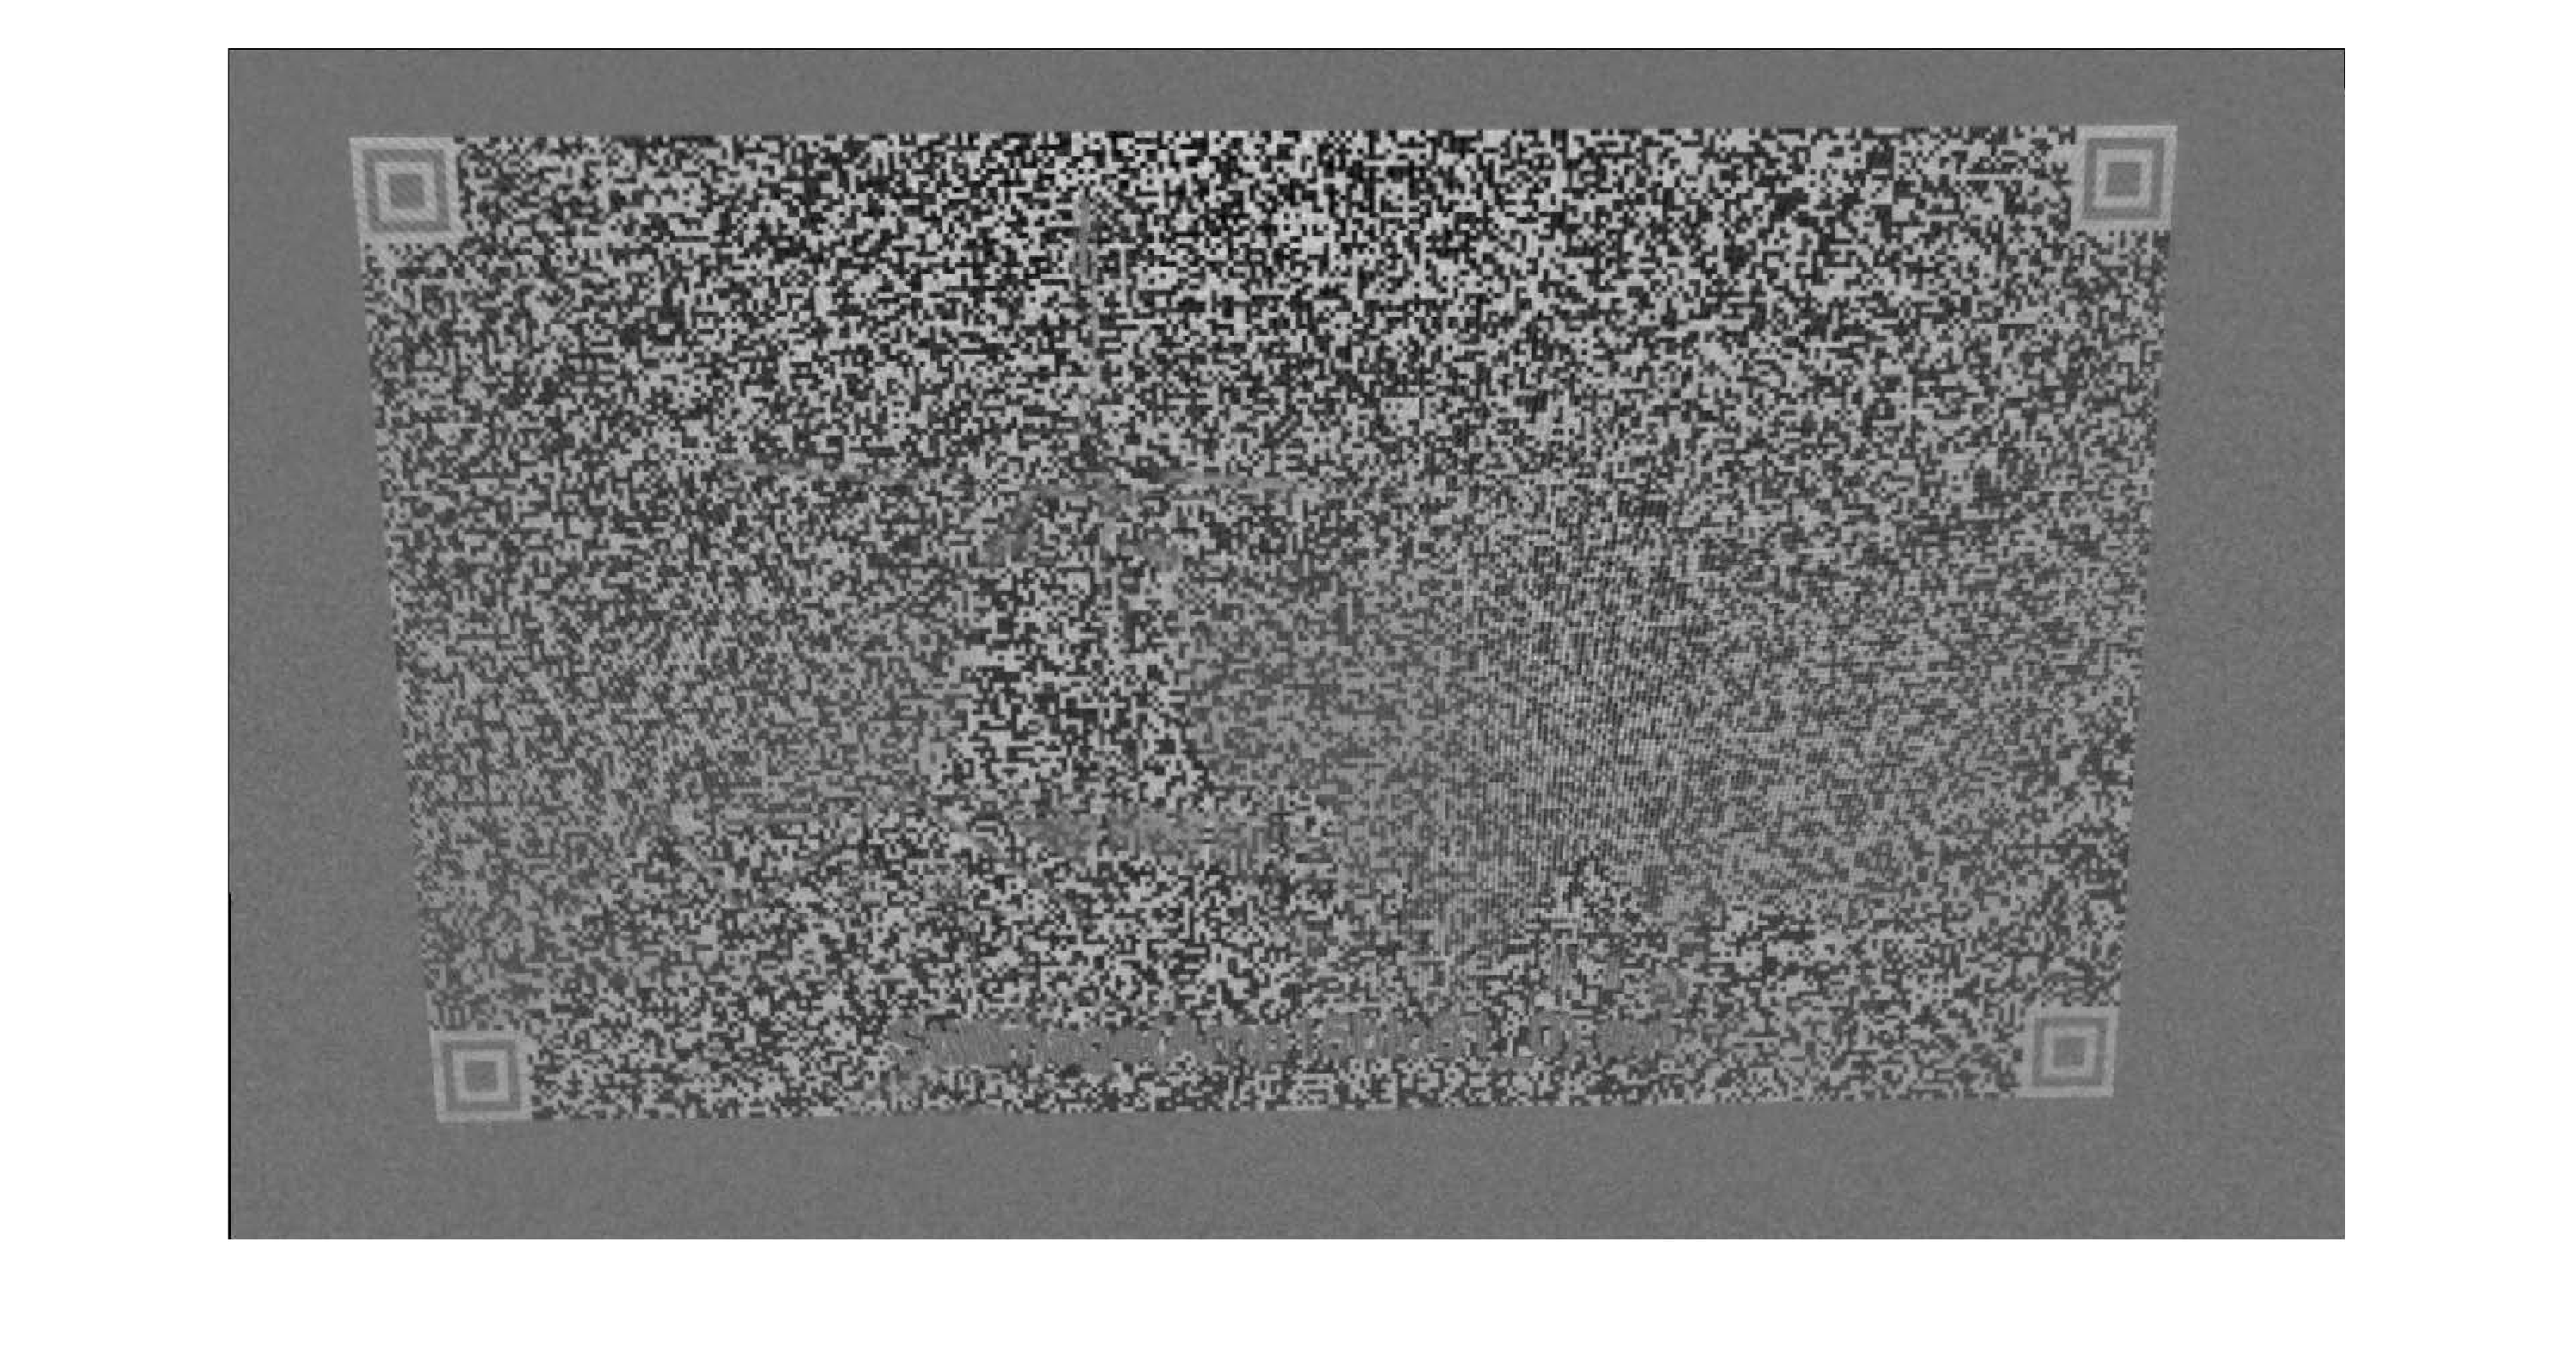
\includegraphics[keepaspectratio,width=0.45\textwidth]{images/3_Ersteverfahren/Differenzbild/0schwarz.pdf}
%}
%\caption{Differenzbildern}
%\label{Differenzbildern}
%\end{figure}



%\begin{table}[htb]
%	\captionabove{mögliche Differenzbilder}
%	\label{tbl:differenzbildformel}
%	\footnotesize
%	\centering
%%	\rowcolors{2}{white}{gray!25}	%TUgreen!25 
%	\begin{tabular}{|c|c|}	%p{}m{}b{}clr p{3cm} p{8cm}
%	\toprule
%	\textbf{Differenzbild}\\
%	\midrule
%	  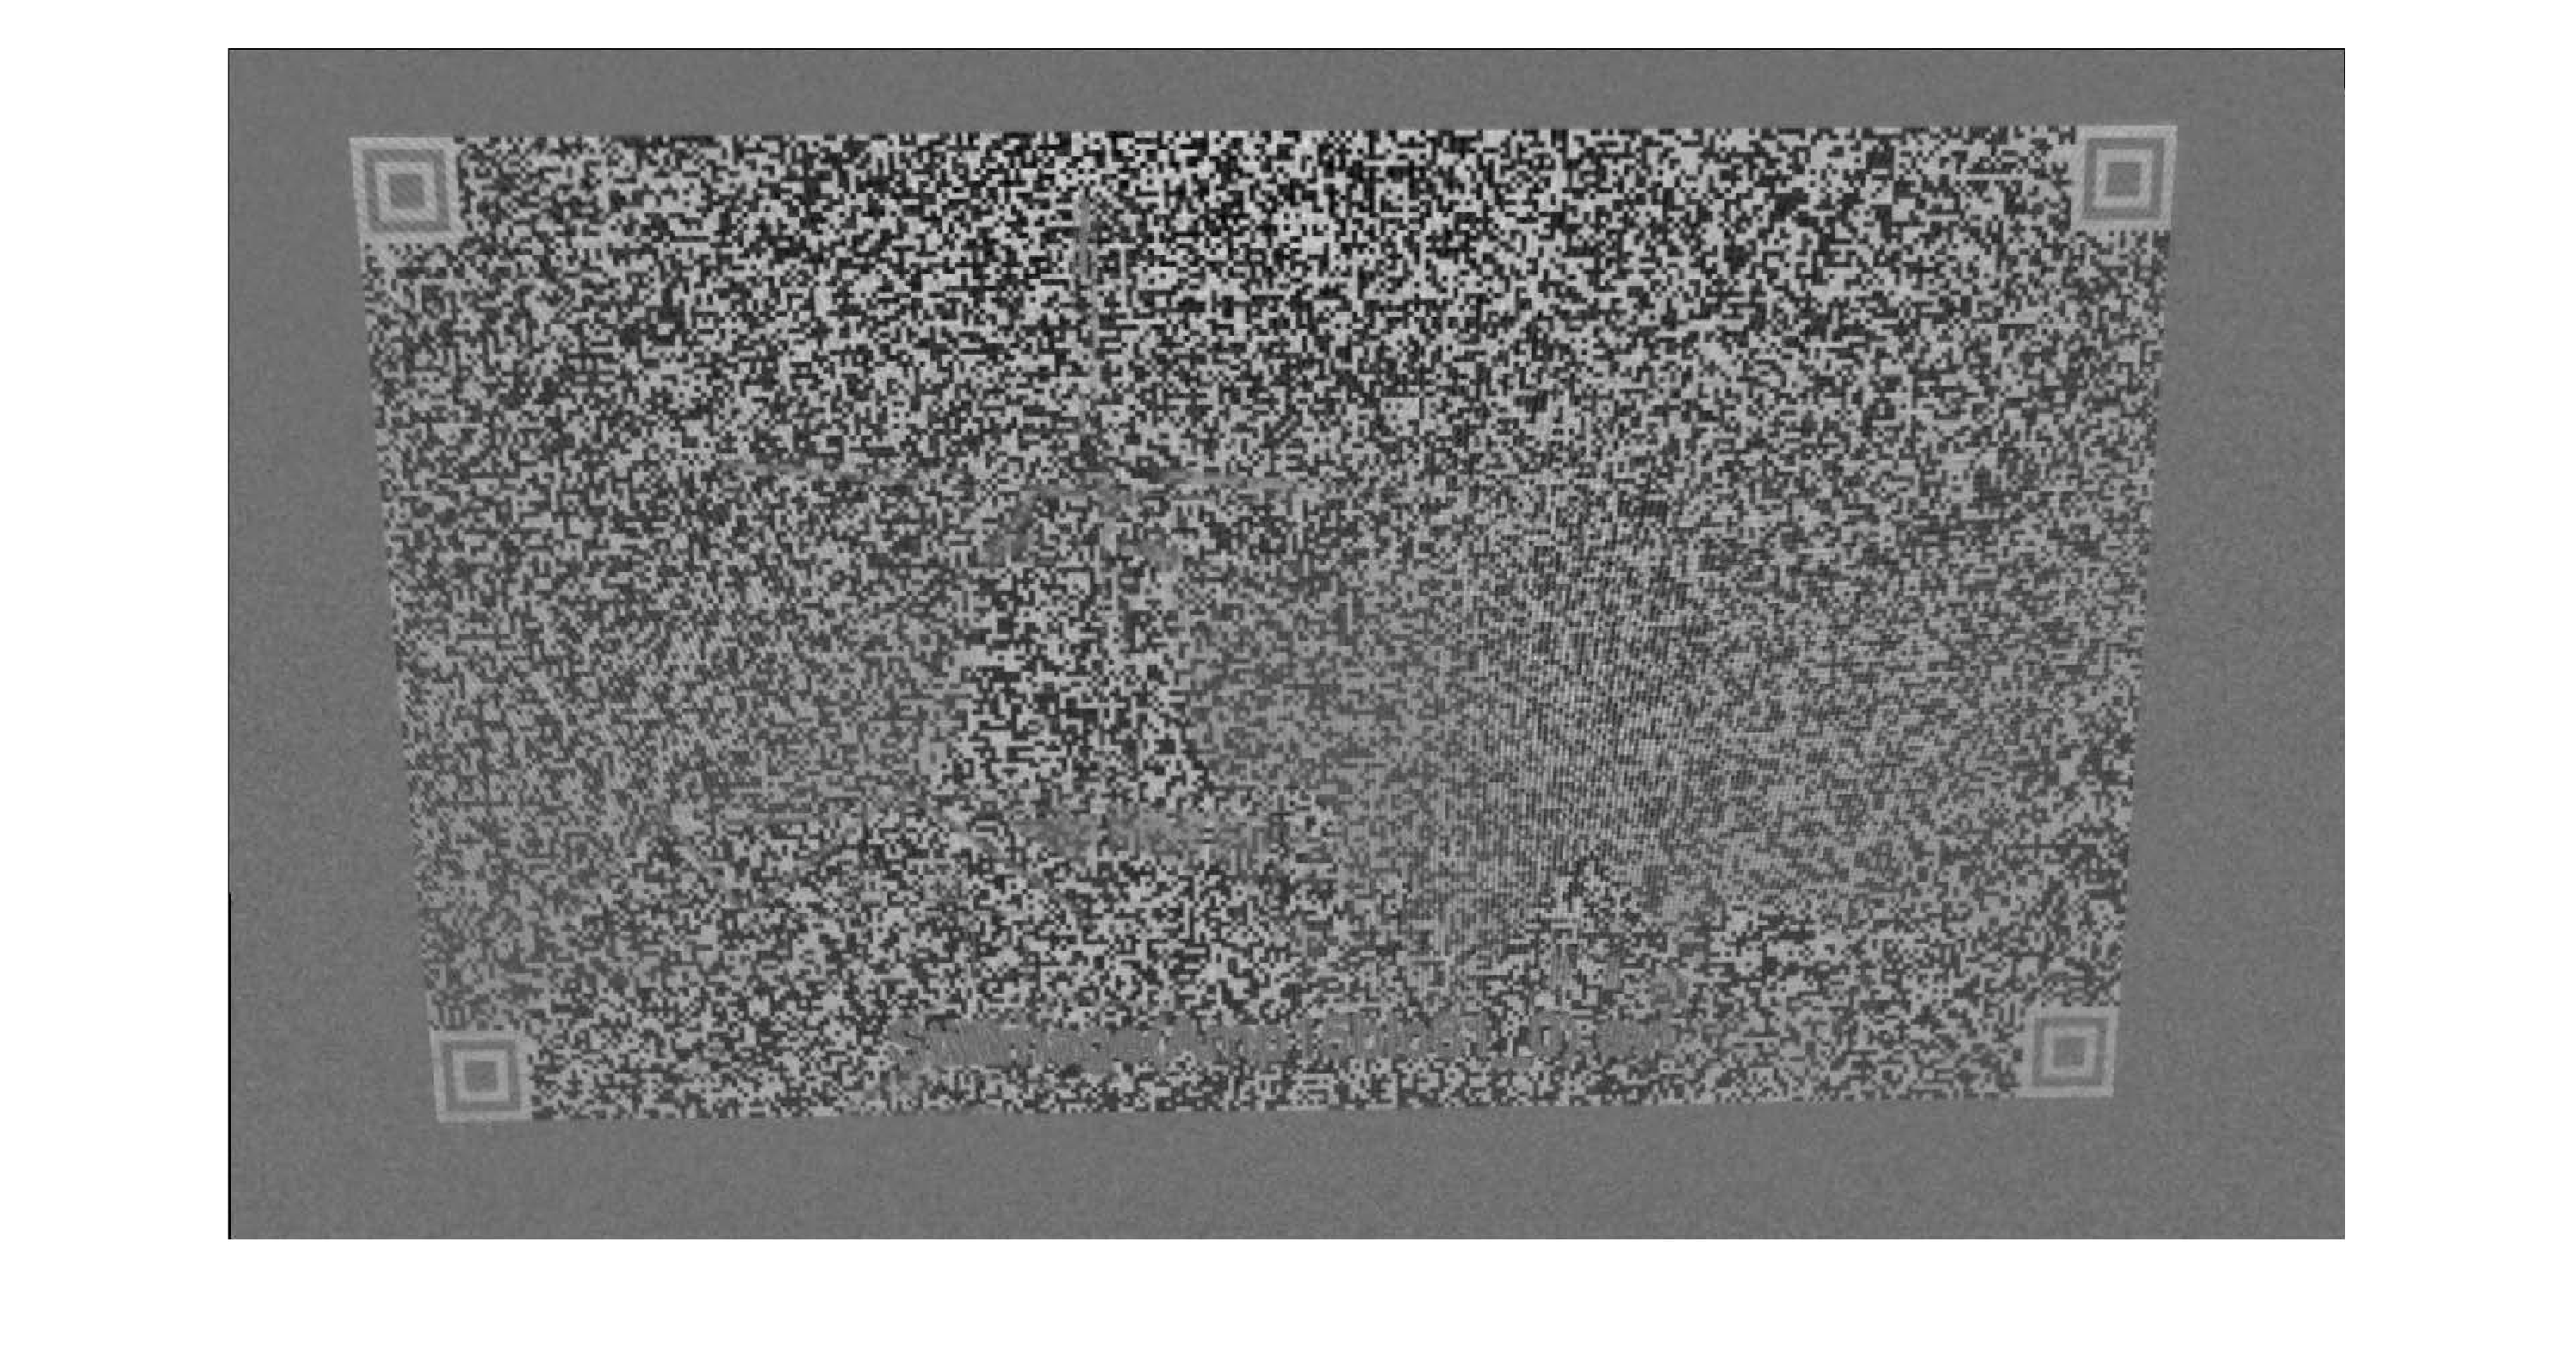
\includegraphics[scale=0.12]{images/3_Ersteverfahren/Differenzbild/0schwarz.pdf} & 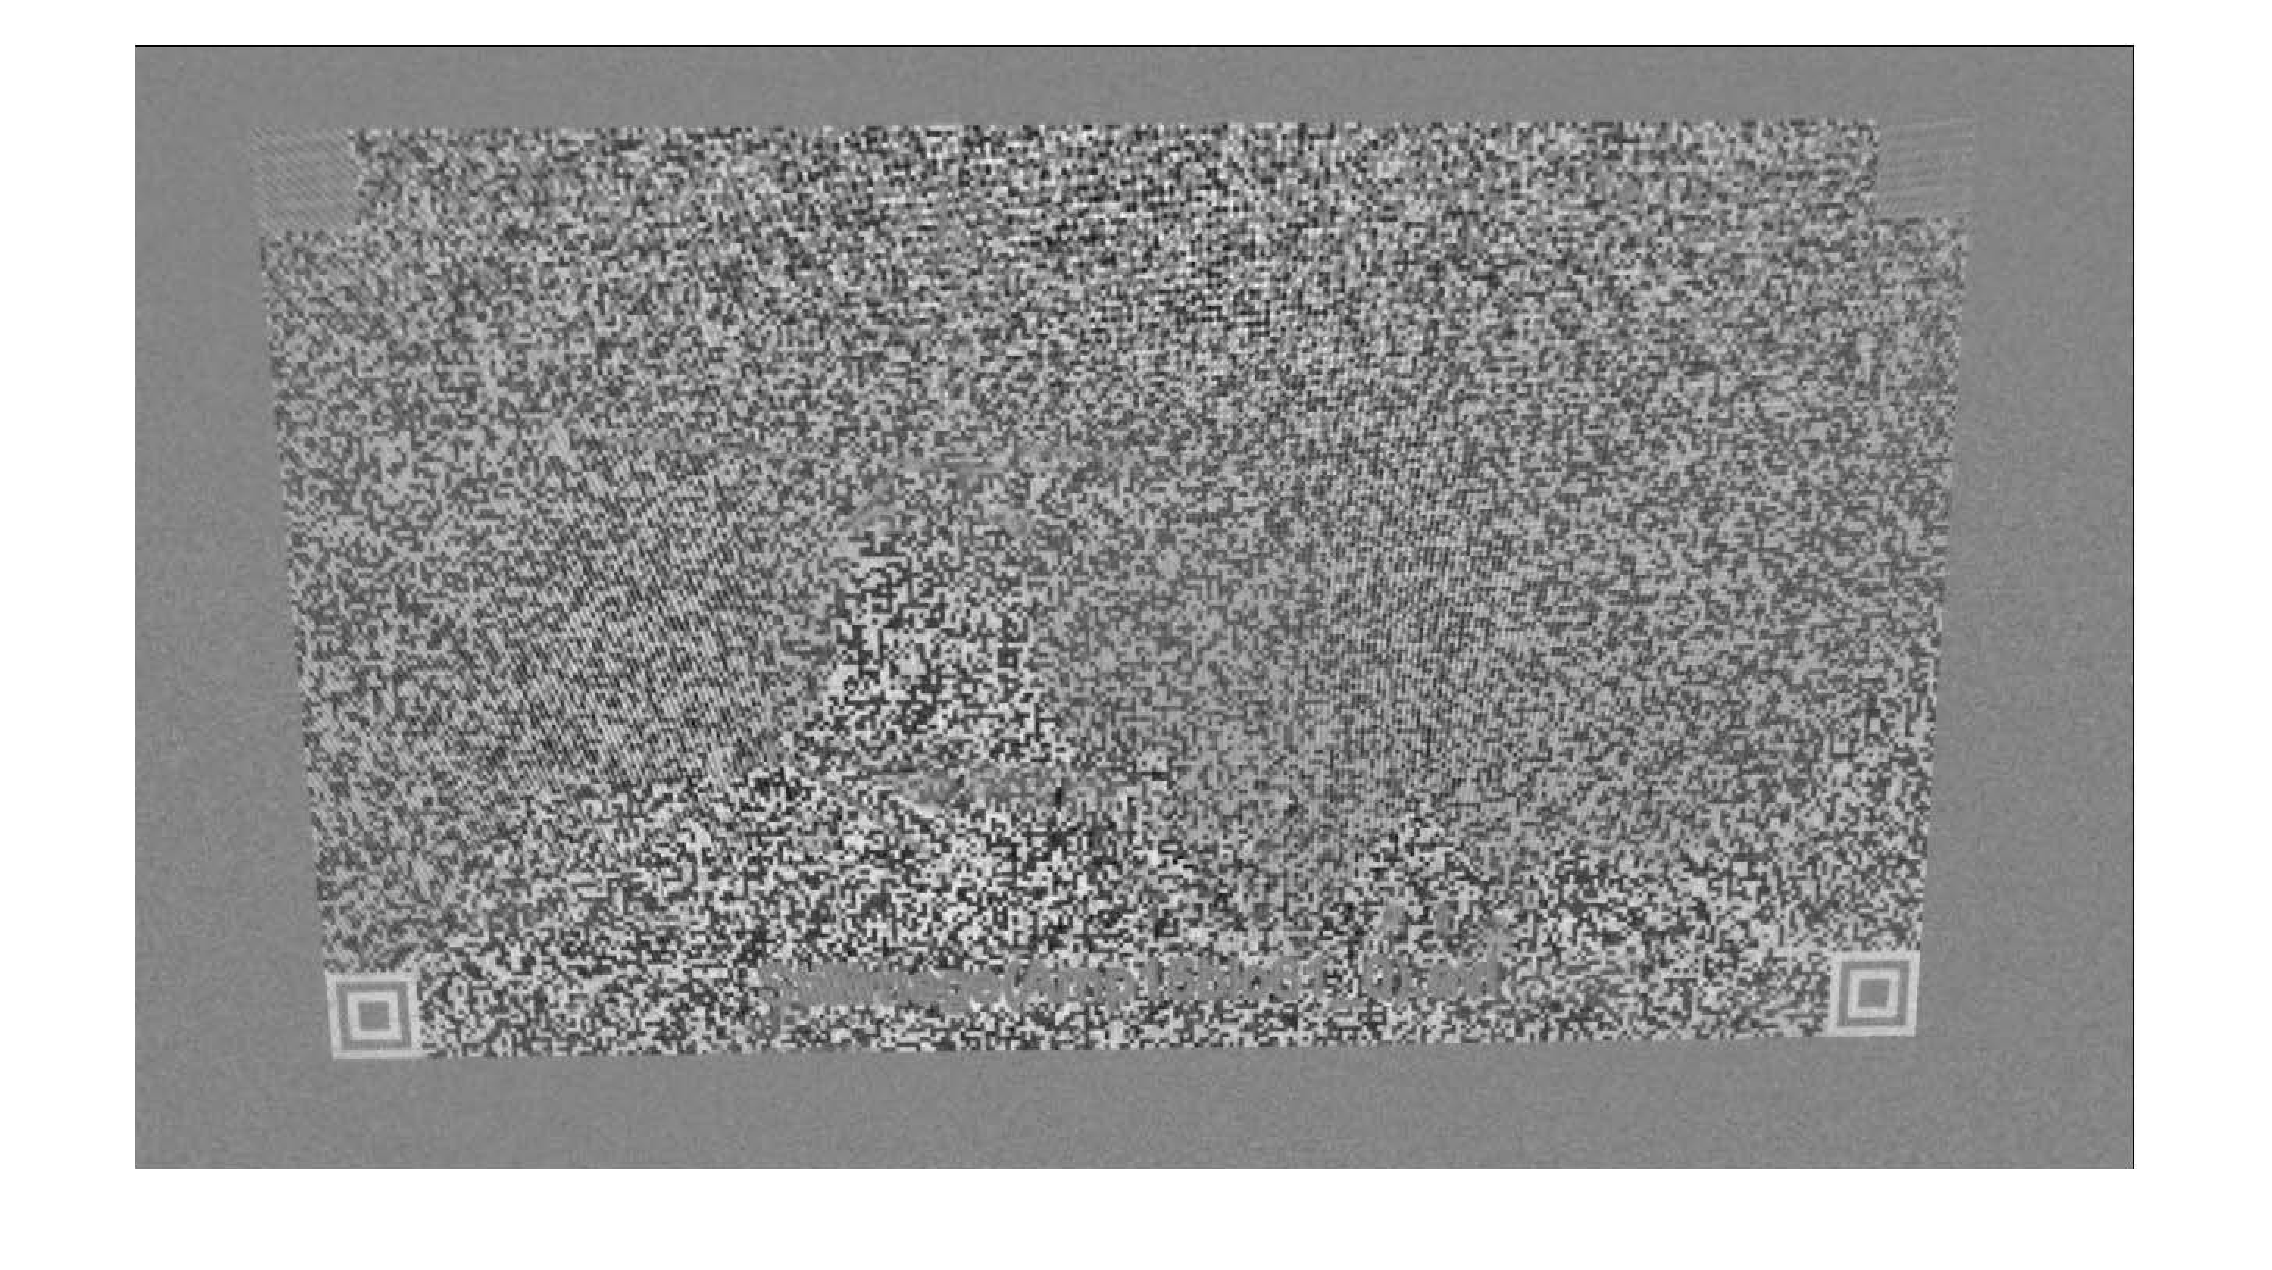
\includegraphics[scale=0.15]{images/3_Ersteverfahren/Differenzbild/1halfschwarz.pdf}\\
%	 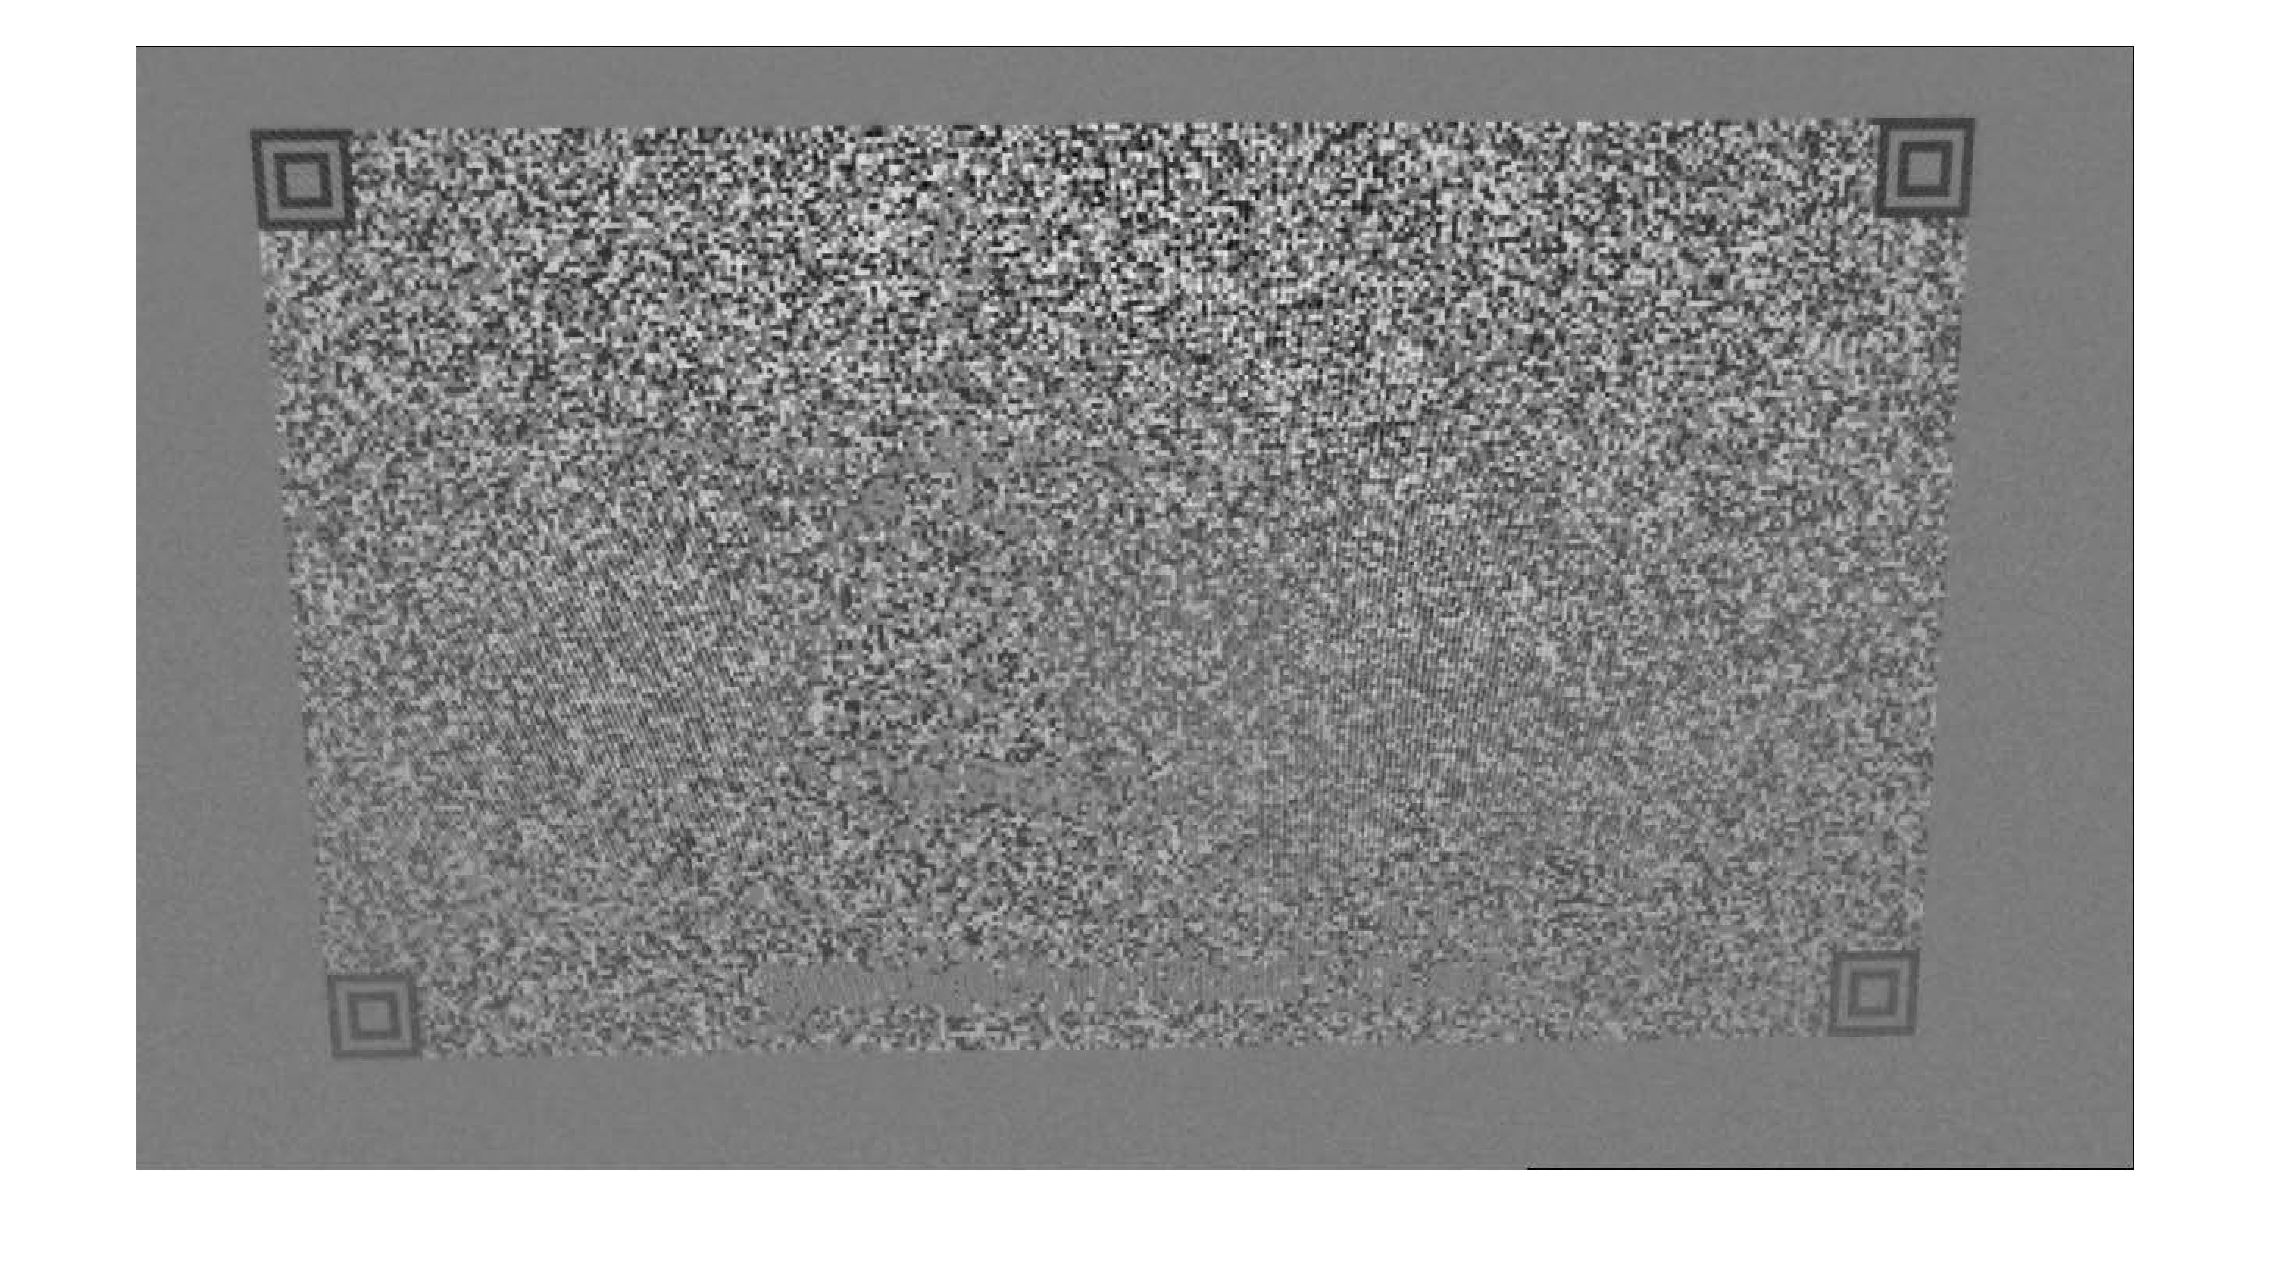
\includegraphics[scale=0.15]{images/3_Ersteverfahren/Differenzbild/2weis.pdf} & 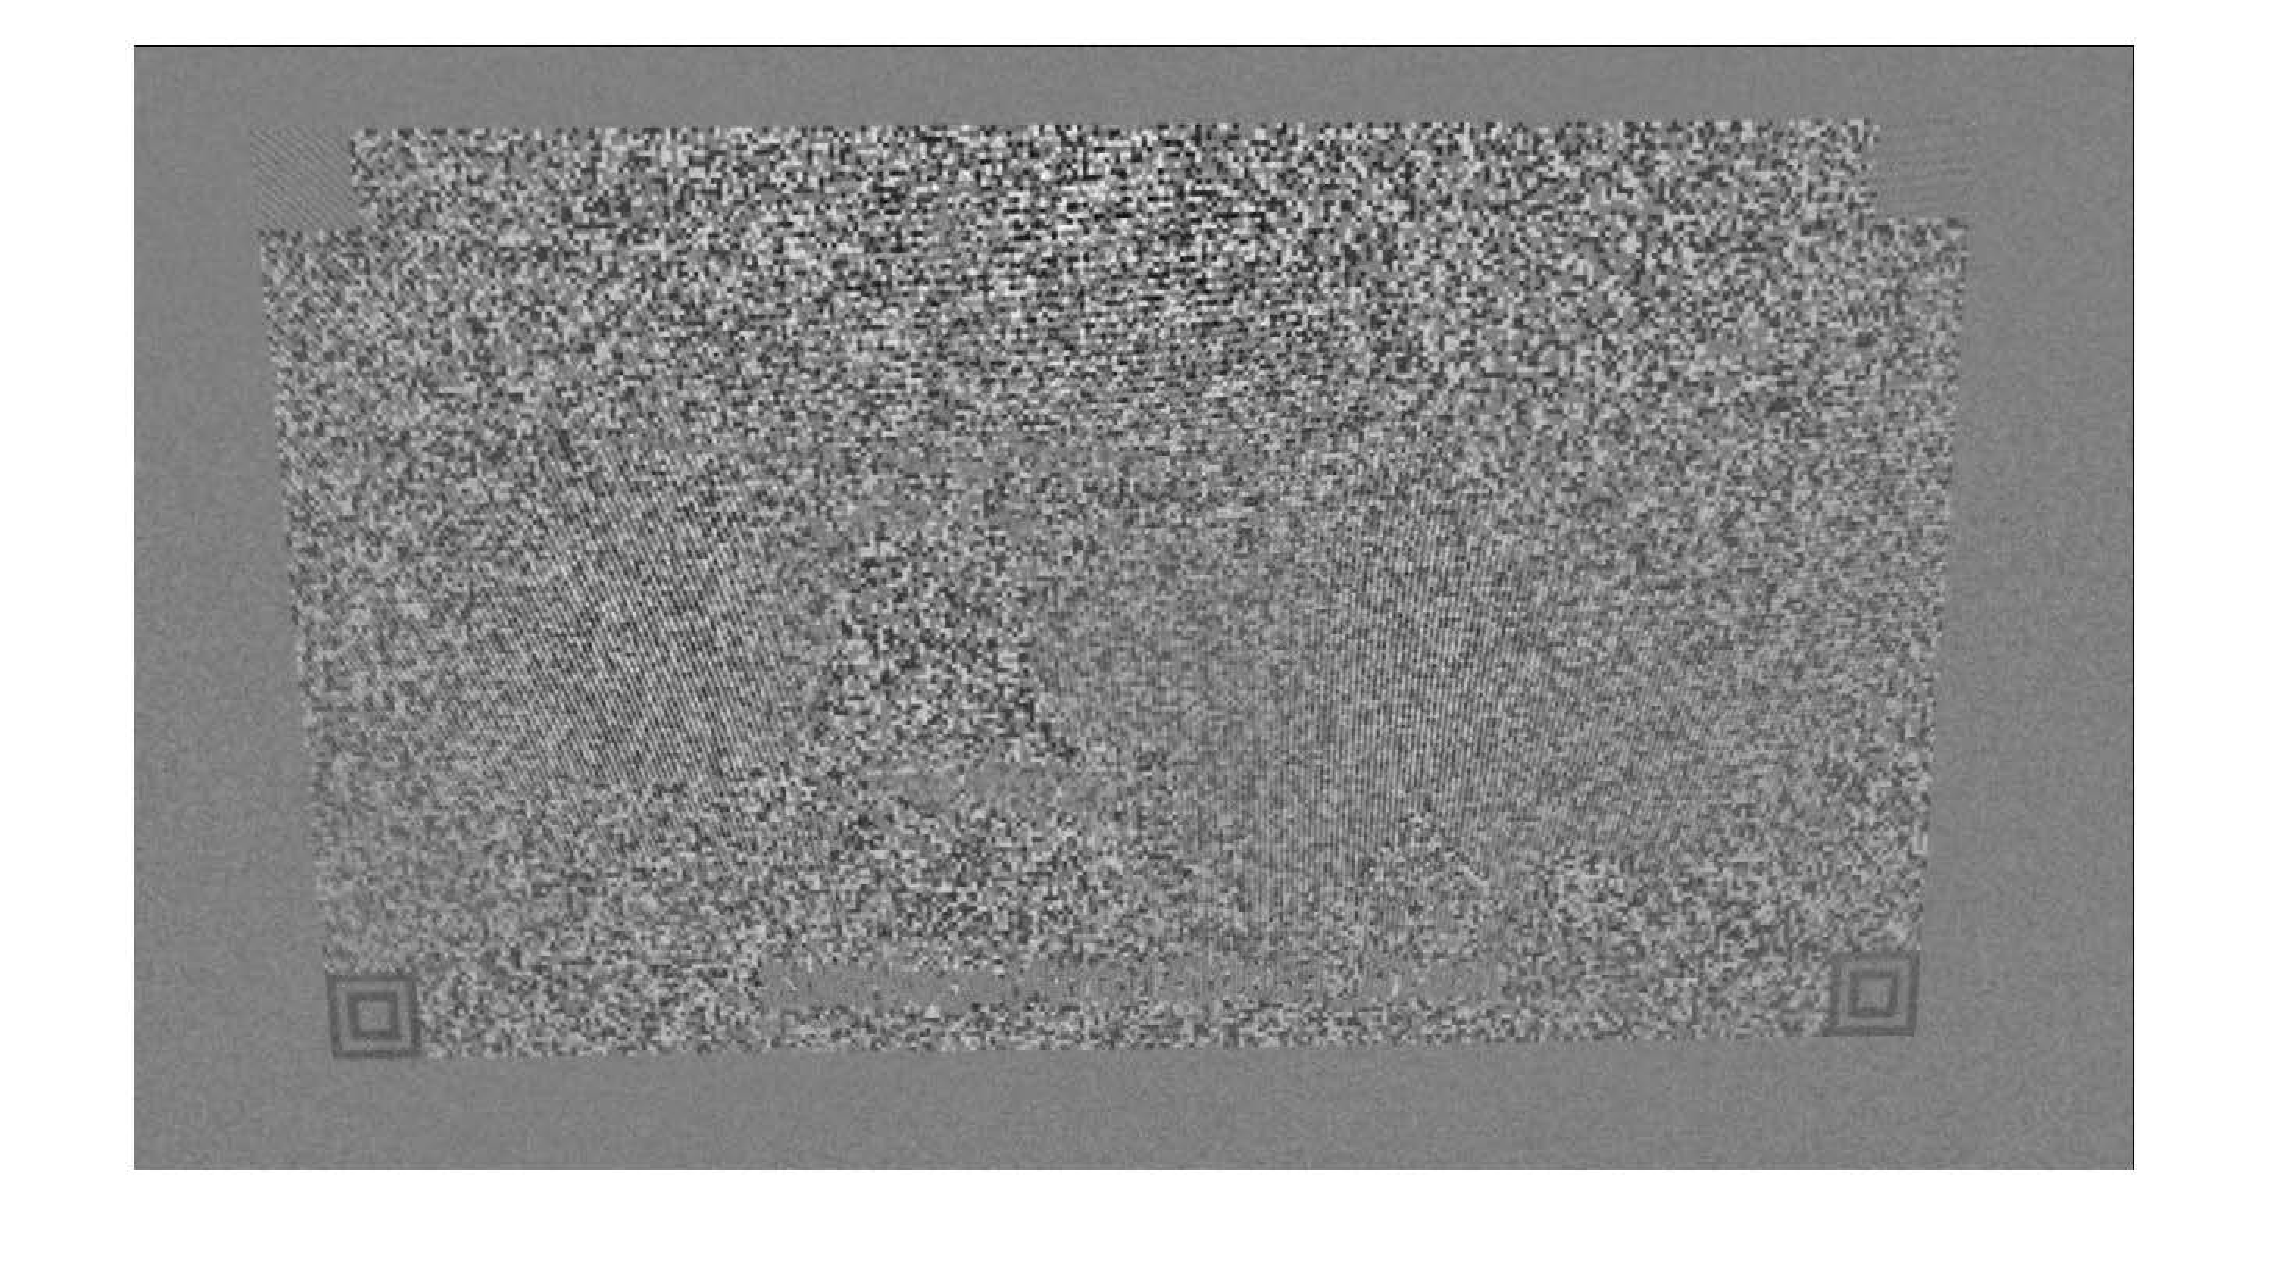
\includegraphics[scale=0.15]{images/3_Ersteverfahren/Differenzbild/3halfweis.pdf}\\
%	 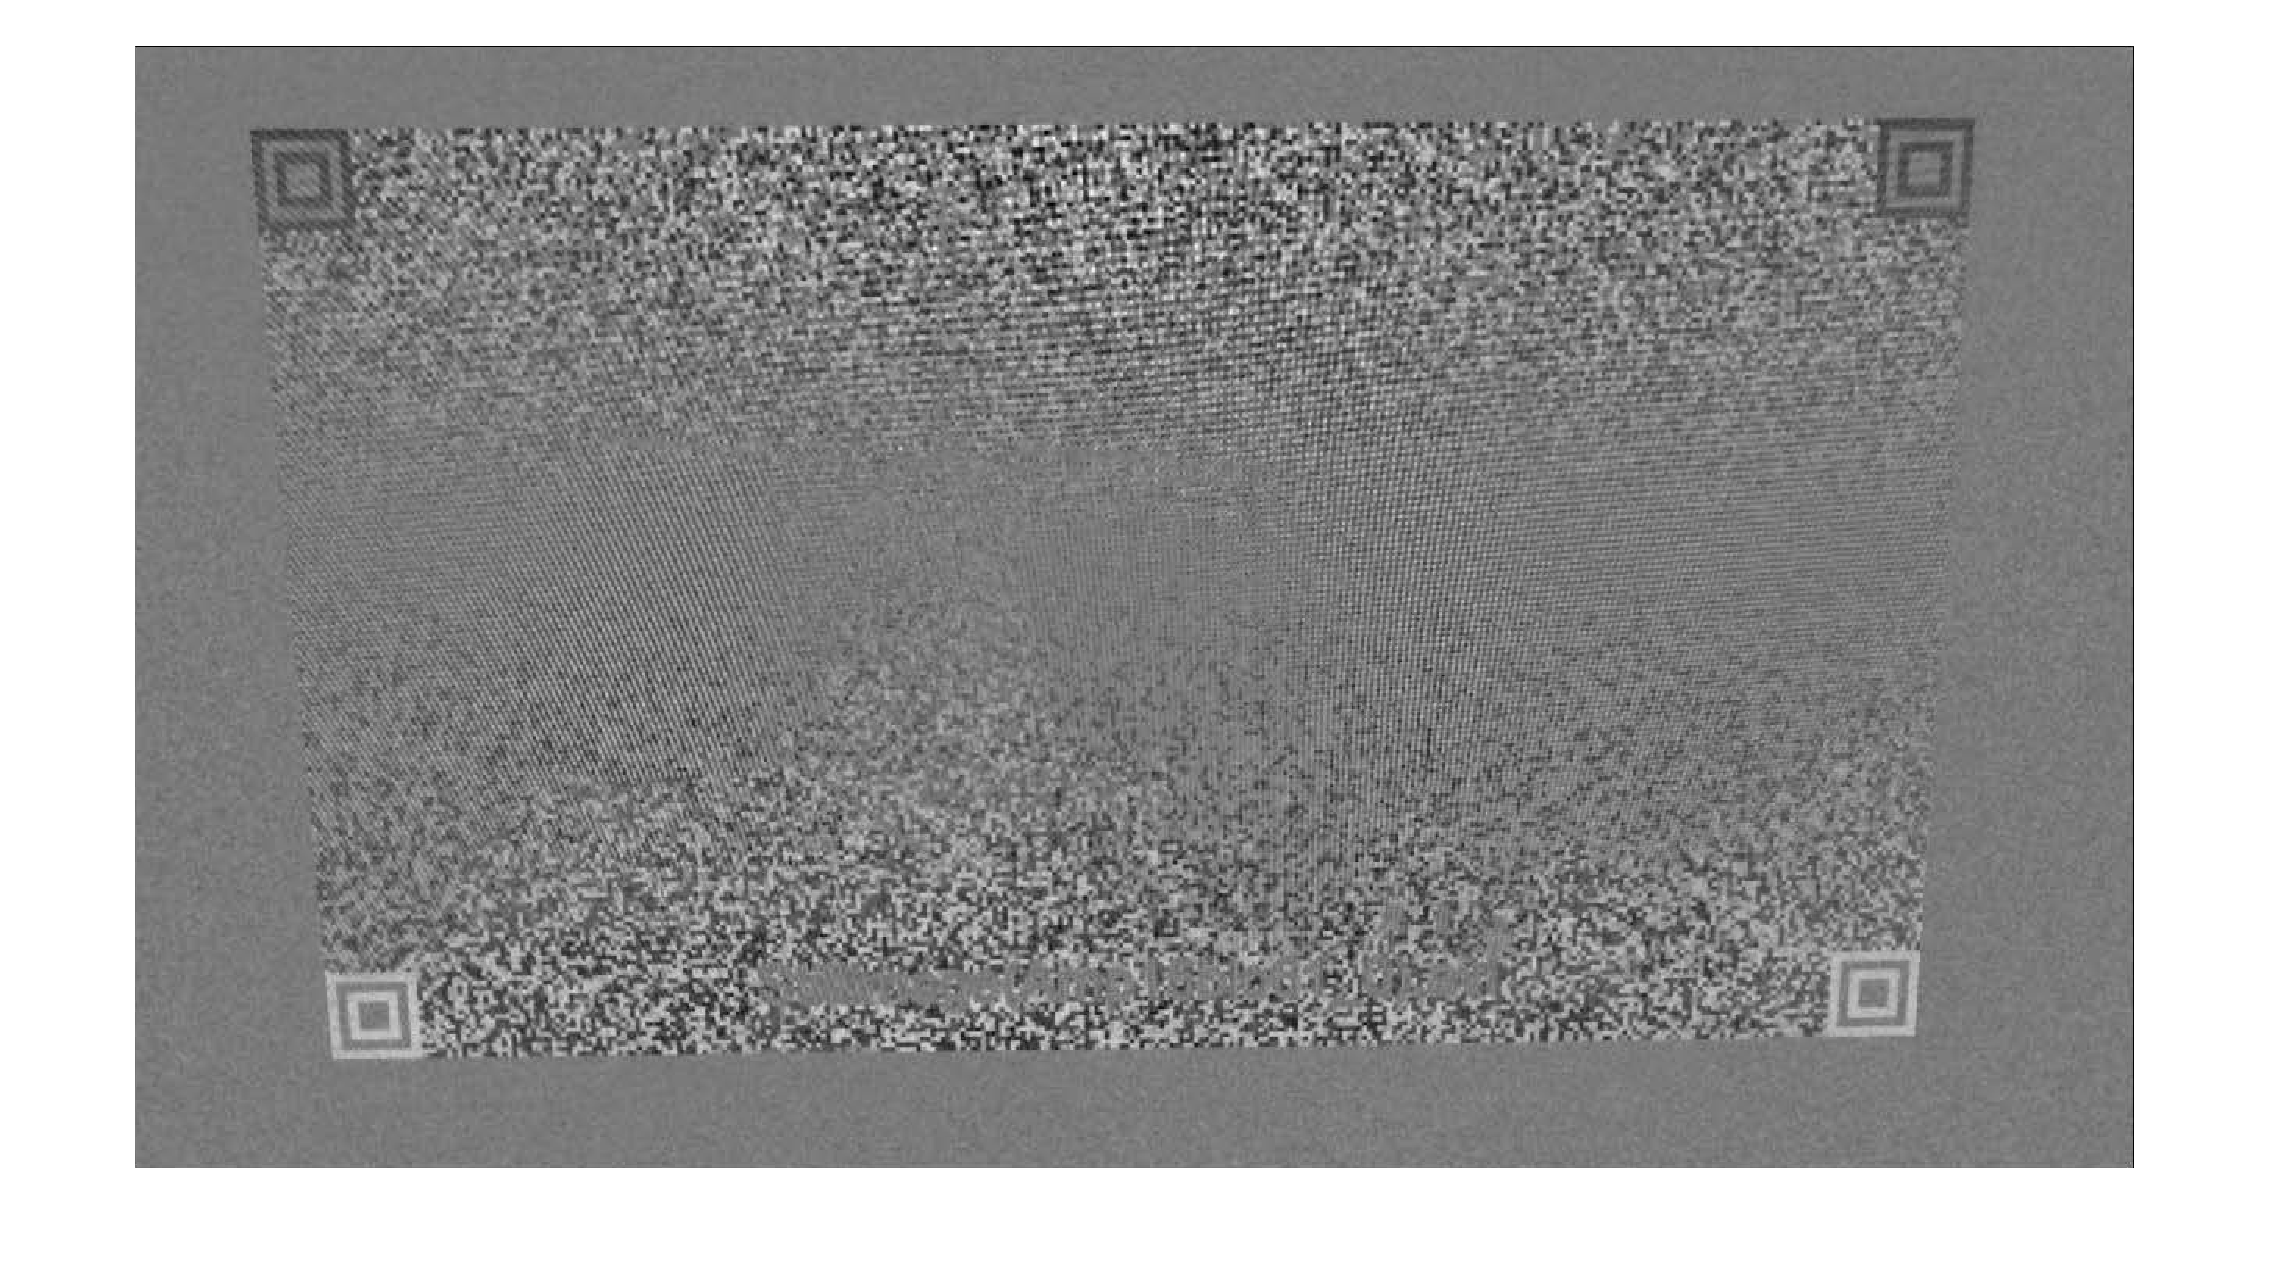
\includegraphics[scale=0.15]{images/3_Ersteverfahren/Differenzbild/4halbschwaryhalbweis.pdf} & 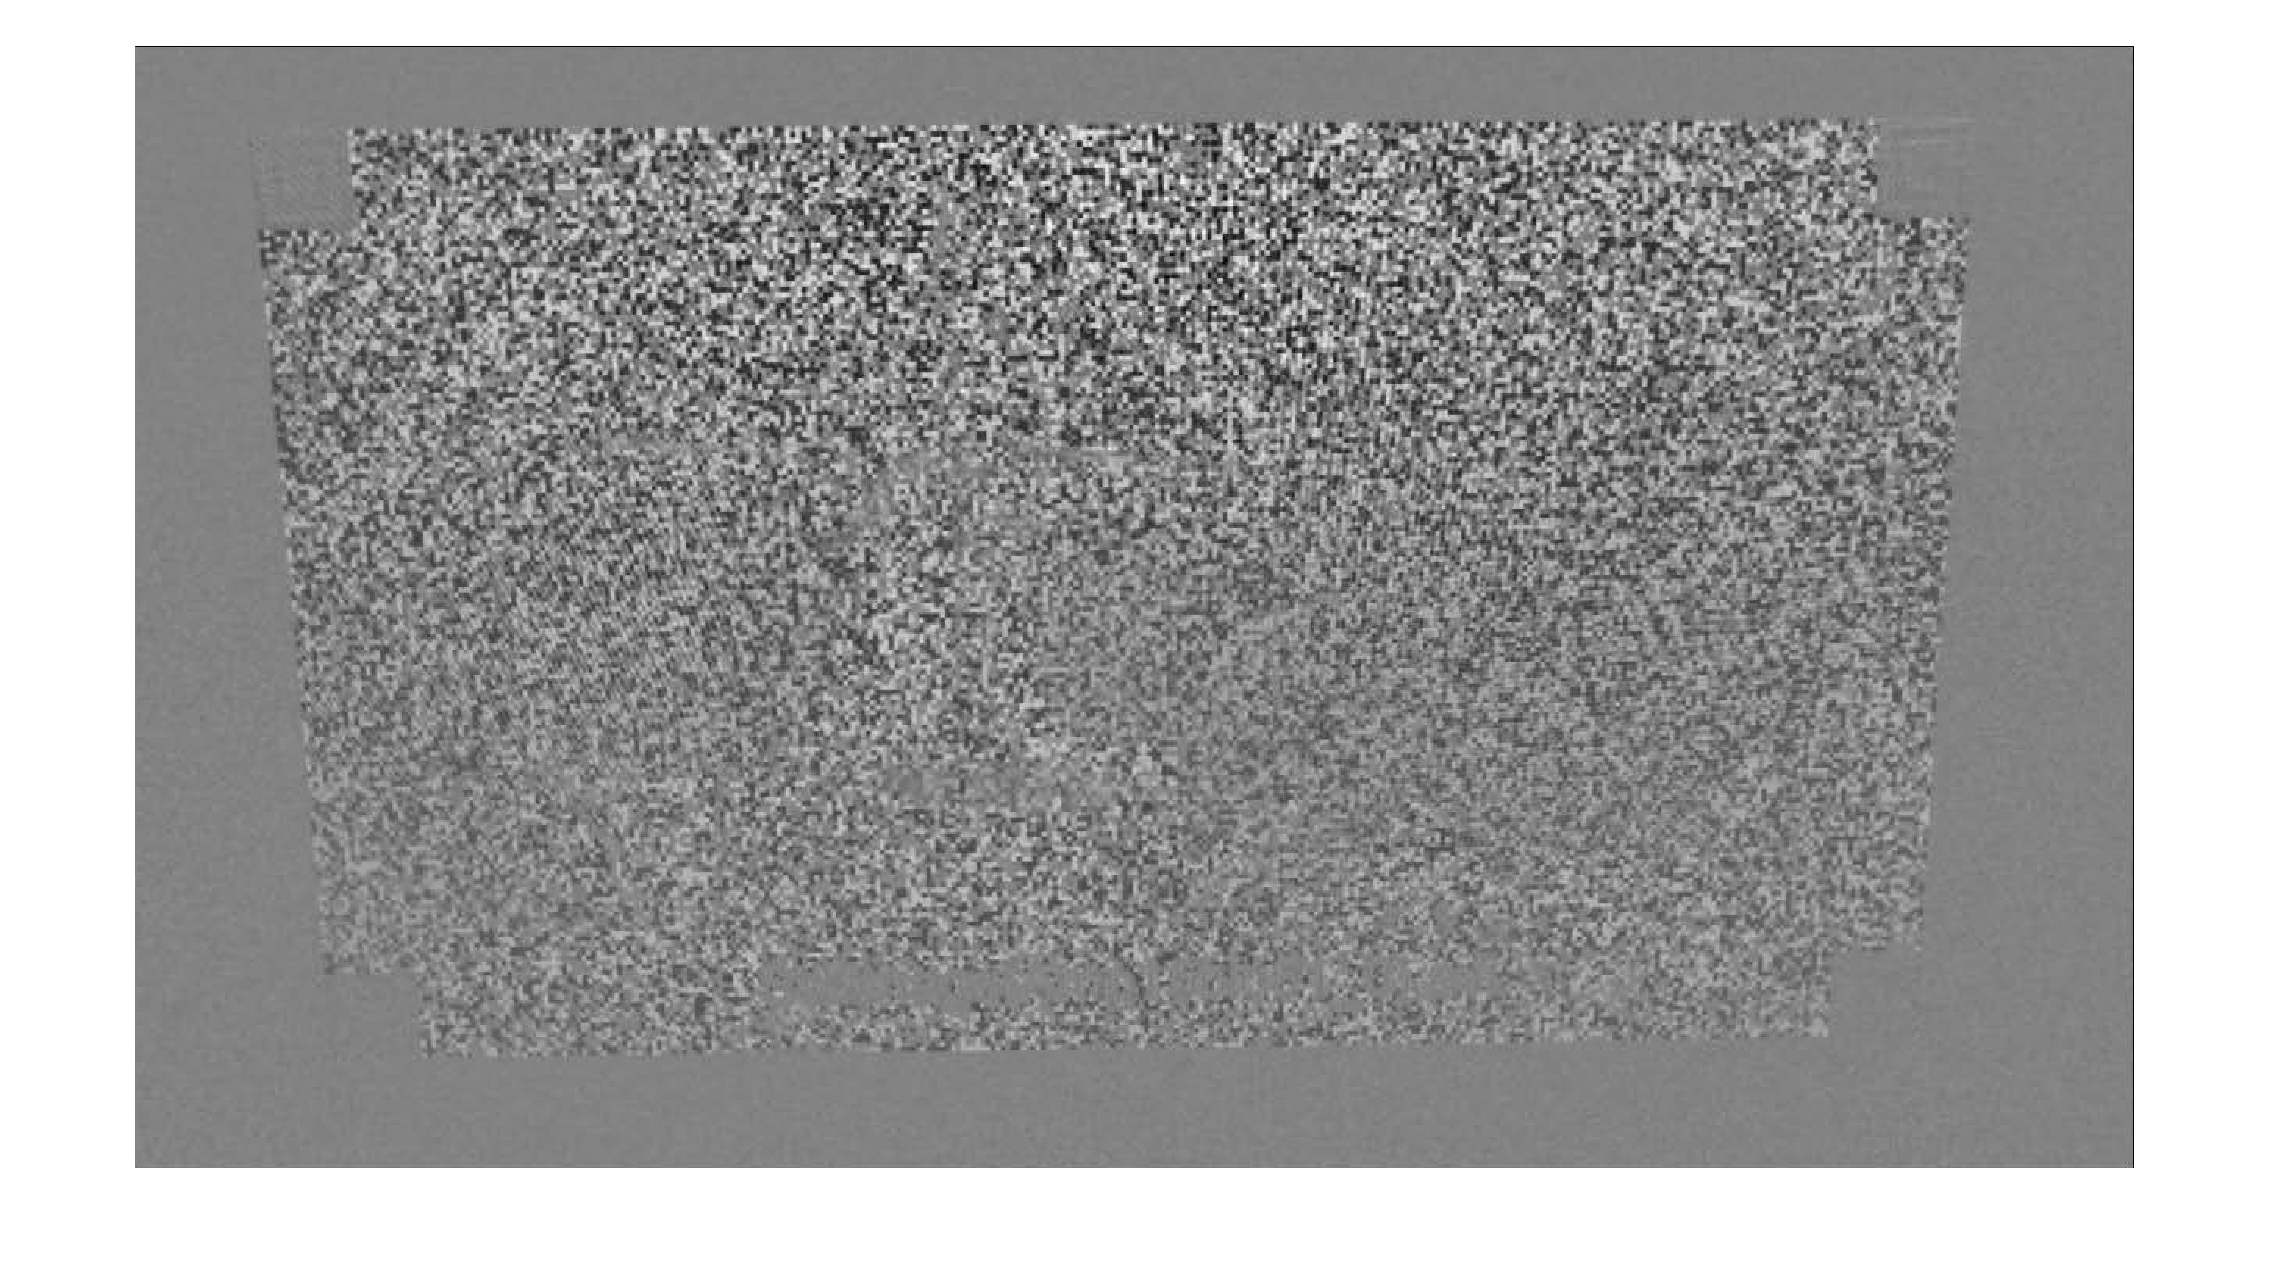
\includegraphics[scale=0.15]{images/3_Ersteverfahren/Differenzbild/5aufheben.pdf}\\
%
%	\bottomrule
%	\end{tabular}
%\end{table} 




\begin{figure}[H]
\centering 
\begin{minipage}[b]{0.49\textwidth} 
\centering 
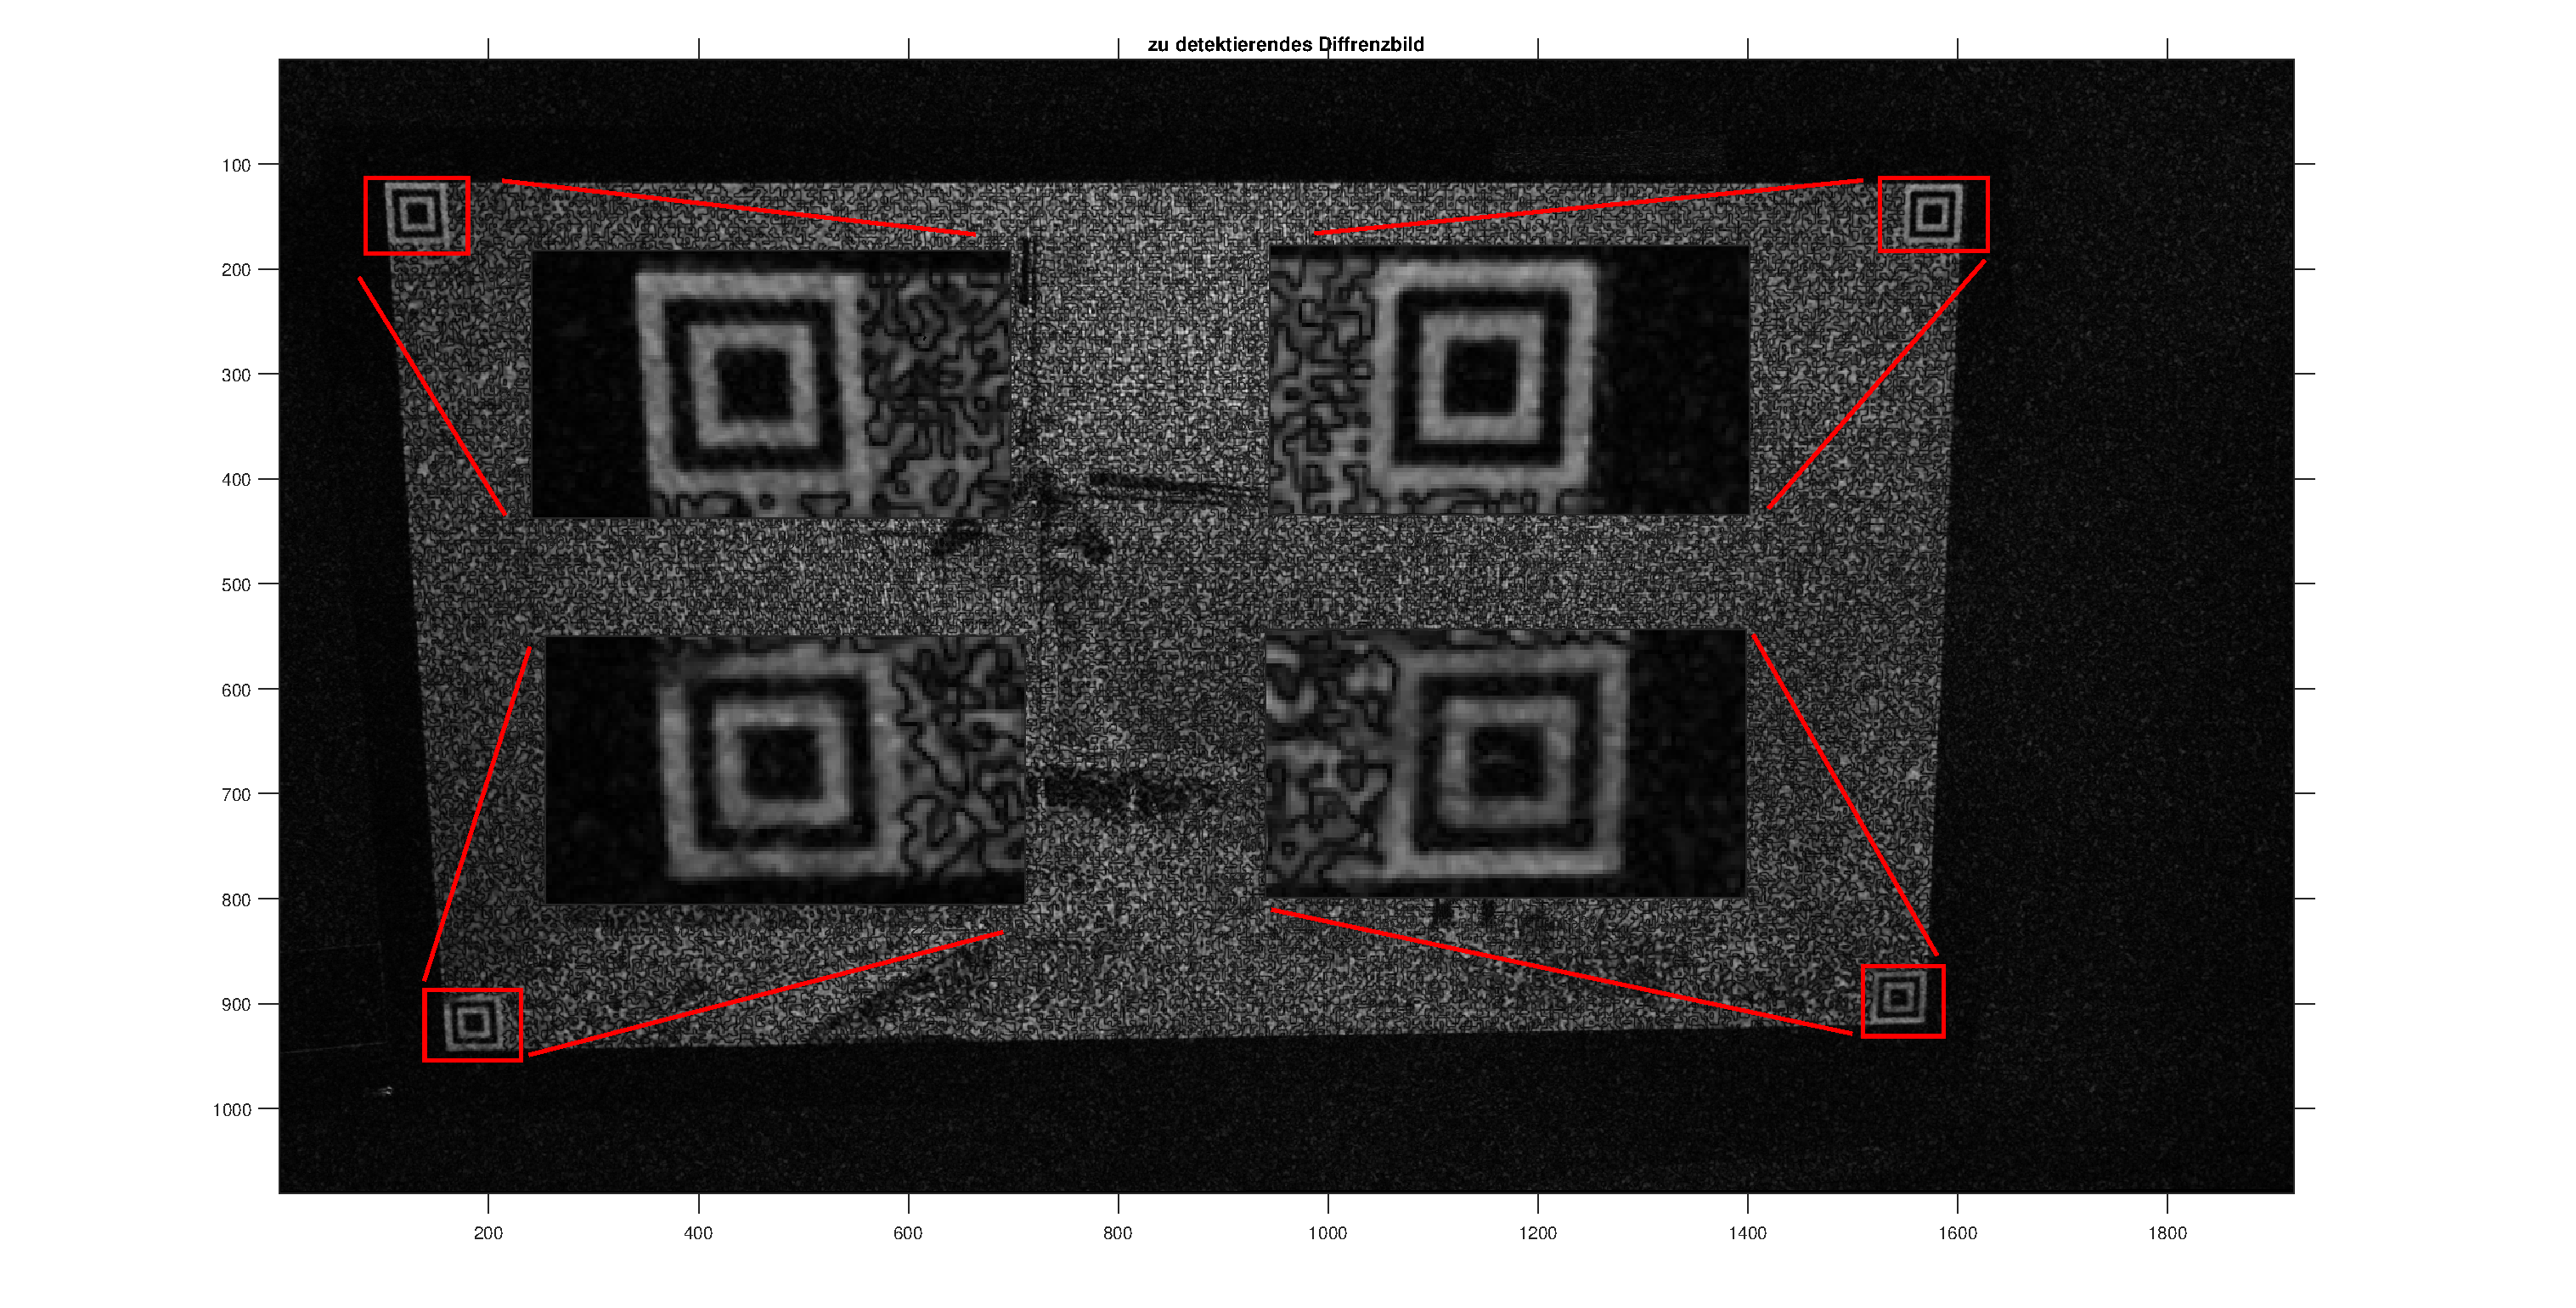
\includegraphics[width=1.0\textwidth]{images/5_Implementirung/Diff/zudifferenzbild.eps} 
\caption{Ein zu detektierendes Bild}
\label{fig:nachdiff}
\end{minipage}
\begin{minipage}[b]{0.49\textwidth} 
\centering 
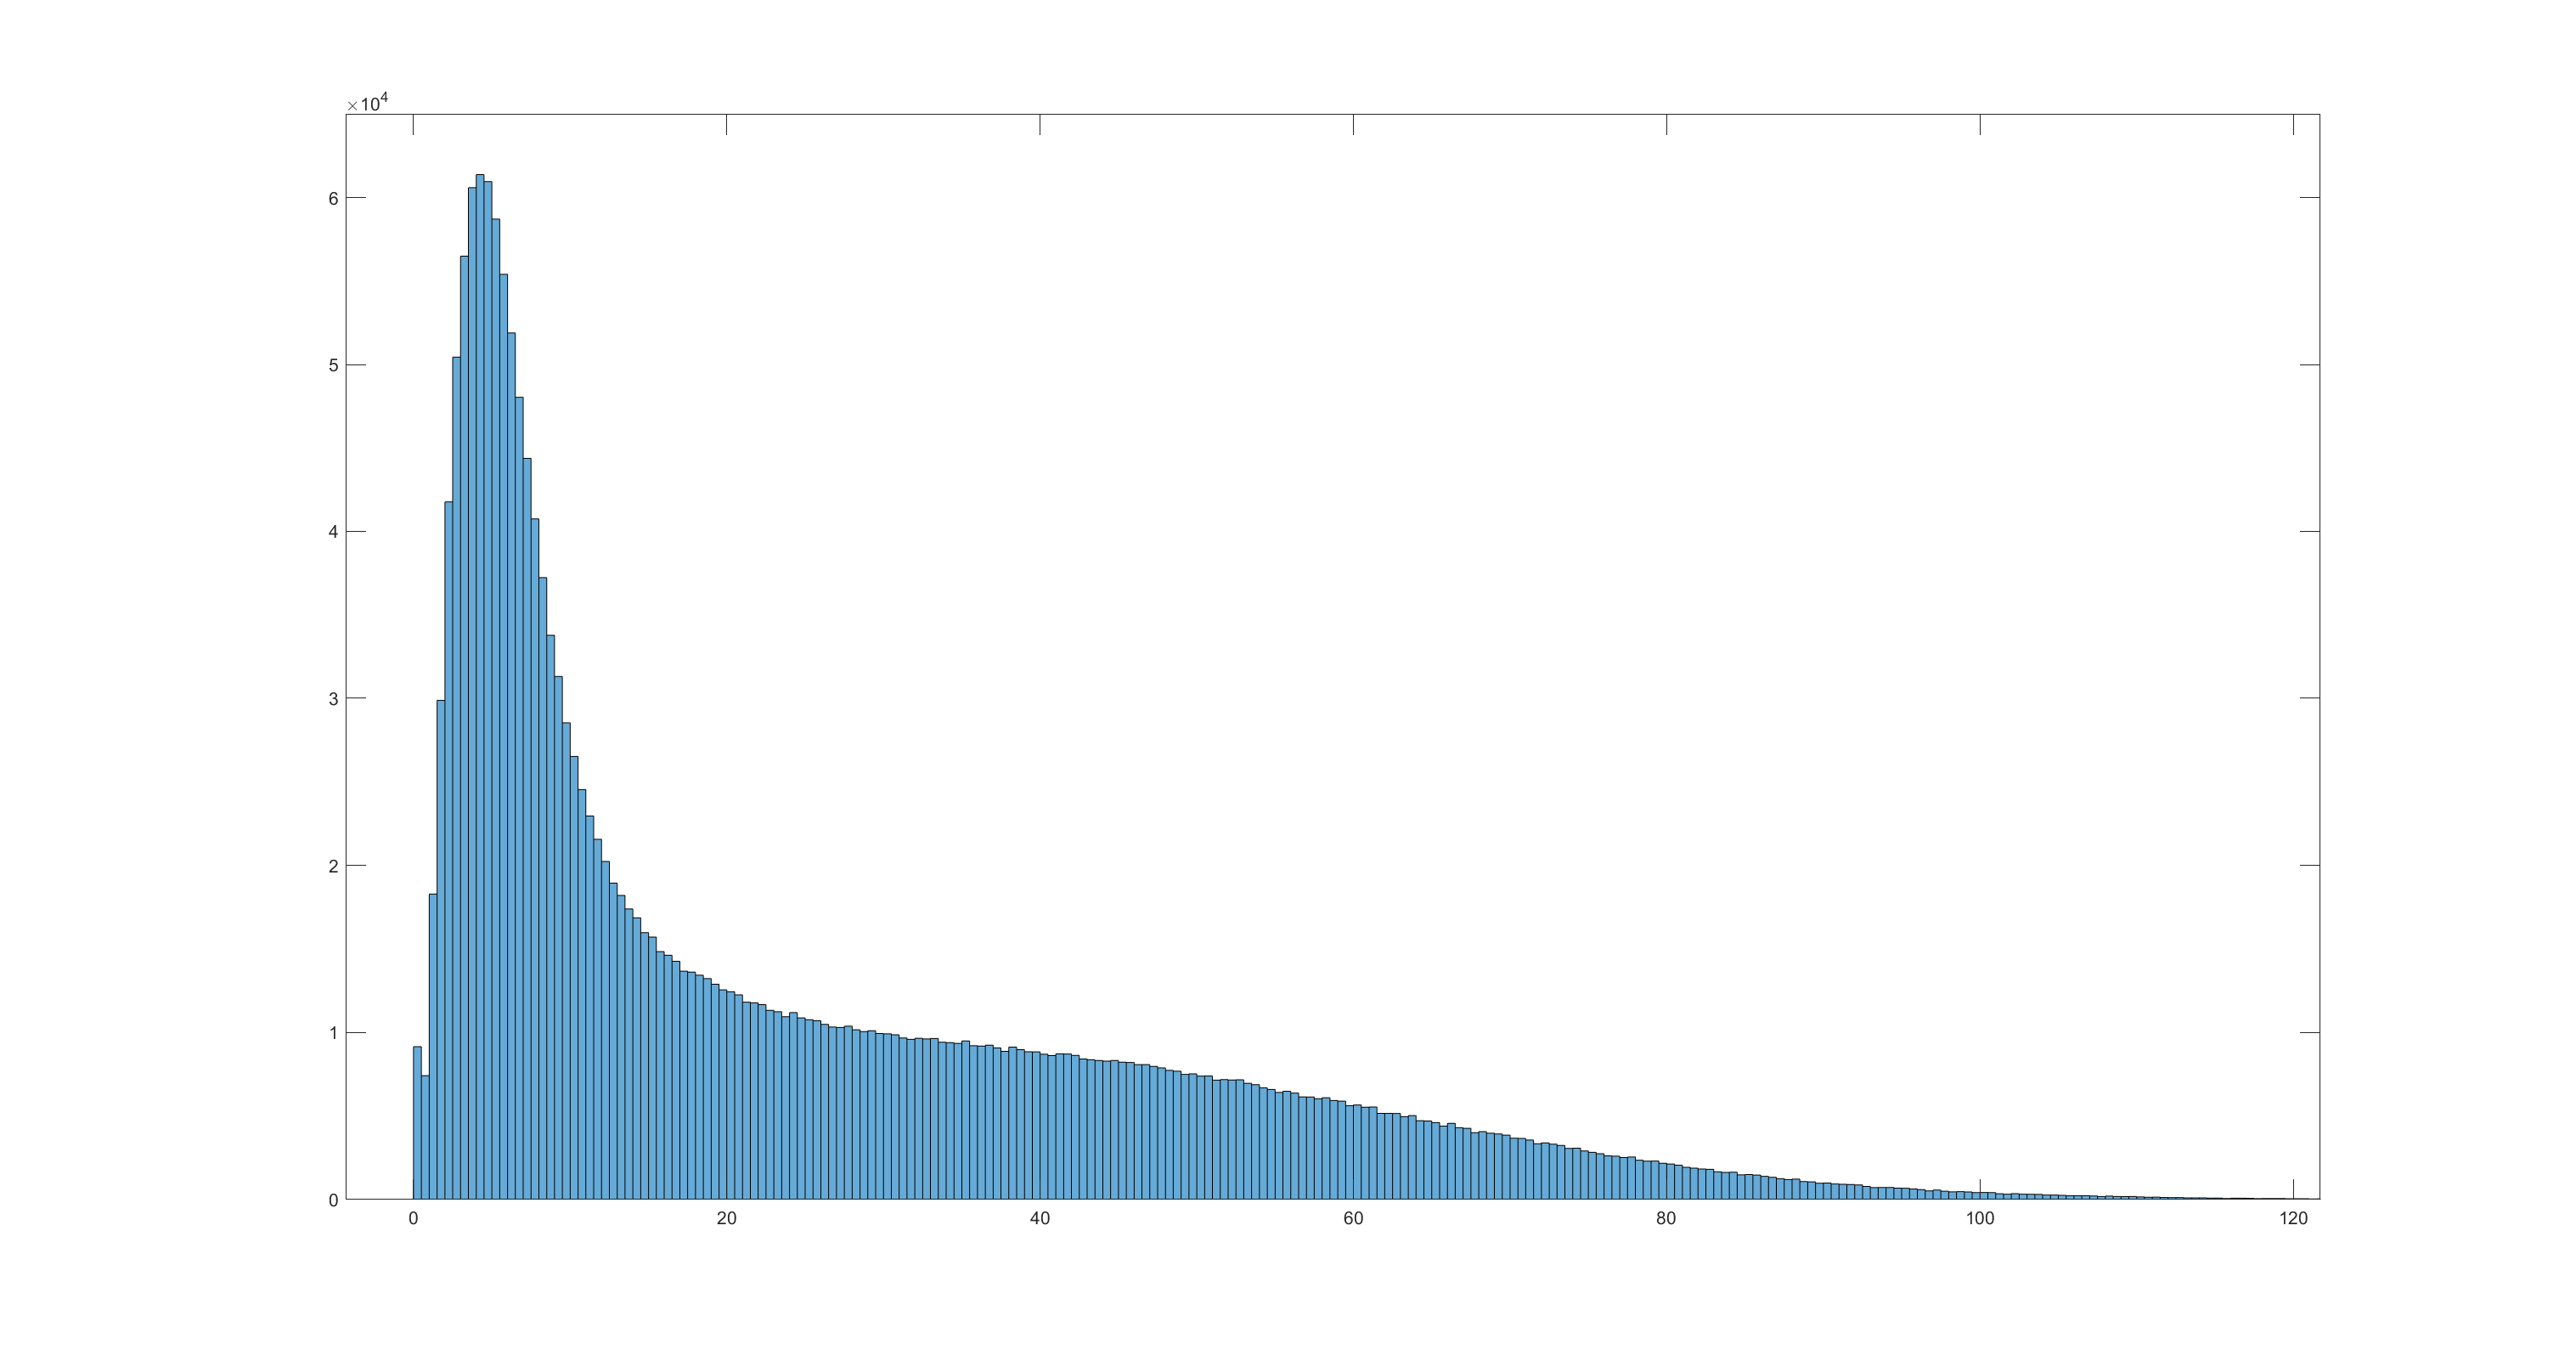
\includegraphics[width=1.0\textwidth]{images/5_Implementirung/Diff/histogramm.eps}
\caption{entsprechendes Histogramm}
\label{fig:Histogramm}
\end{minipage}
\end{figure}

Anschließend wird das Bild zur Bildverarbeitung durchgeführt. Abbildung \ref{fig:binar} und Abbildung \ref{fig:morpho} zeigen die Ergebnisse durch die Binarisierung bzw. durch die Morphologie Operation. Nach der Binarisierungsvorgang mit Ostu wird der Modulationsbereich vom Bild grob extrahiert. Die nächste Morphologie Operation kann die Lücken und die kleine Punkte vom Rauschen stark reduziert. Hier wird ein $ 5 \times 5 $ quadratisches Strukturelement verwendet. Mit der QR Muster Detektion kann das Zentrum des Musters bestimmen werden, wie in Abbildung \ref{fig:QR_muster} zu sehen ist. Dadurch lässt sich der Modulationsbereich bestimmen. In Abbildung \ref{fig:Mudulaitionbereich} wird der Modulationsbereich durch ein rotes Rechteck gekennzeichnet. Schließlich kann mit einer projektiven Transformation das Endergebnis, welche in Abbildung \ref{fig:Ergebnis1} zu sehen ist, erhalten werden.

\begin{figure}[H]
\centering 
\begin{minipage}[b]{0.49\textwidth} 
\centering 
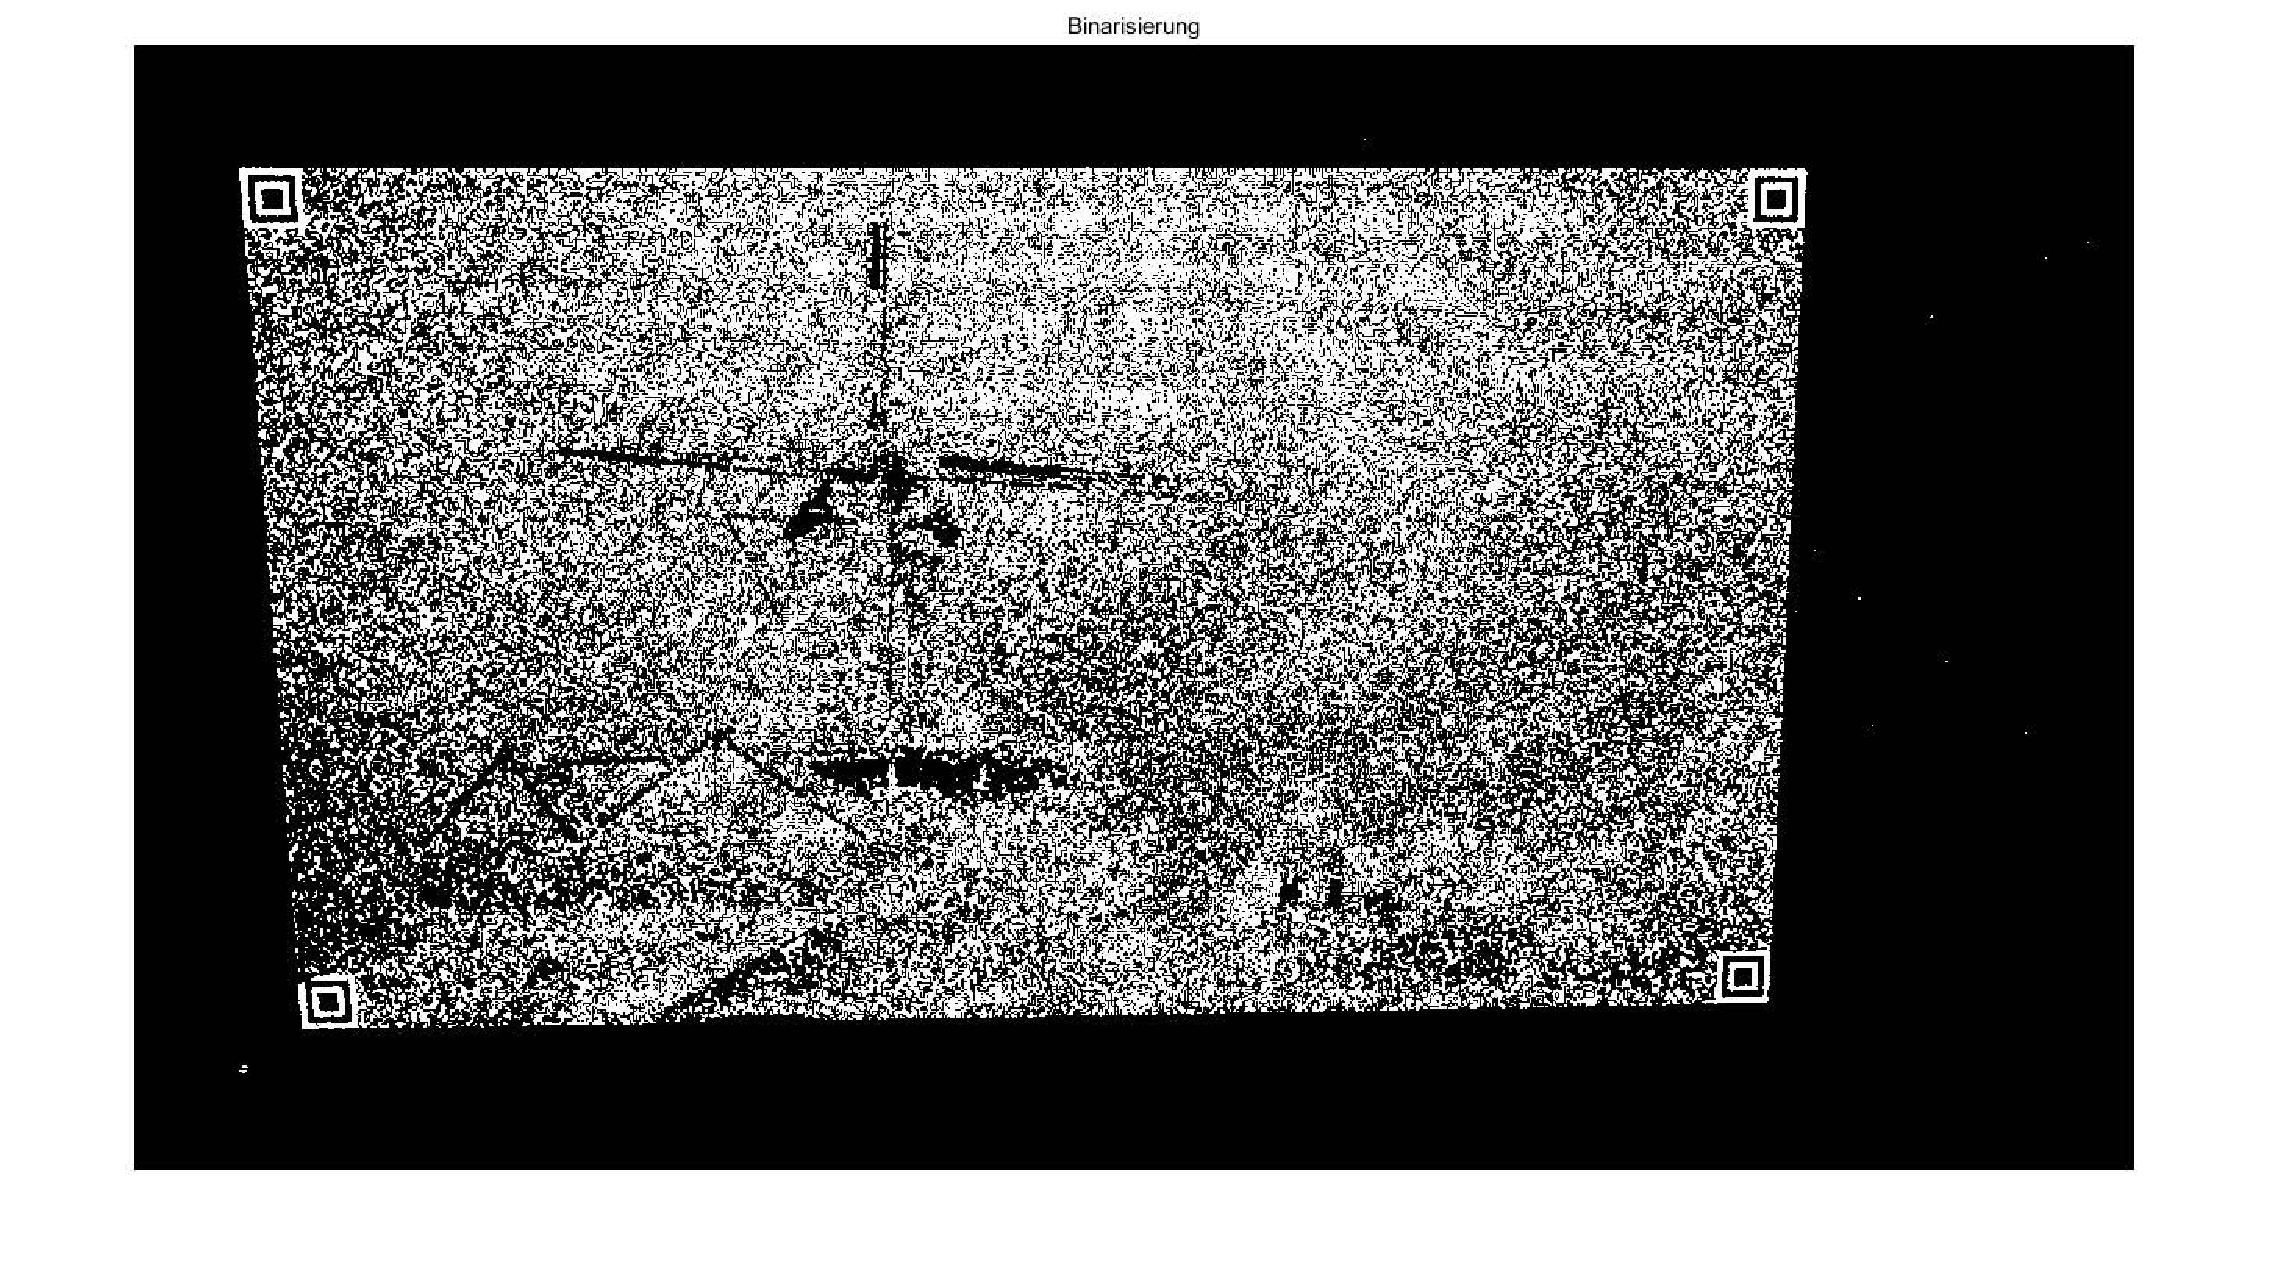
\includegraphics[width=1.0\textwidth]{images/5_Implementirung/Binar.pdf} 
\caption{Binär}
\label{fig:binar}
\end{minipage}
\begin{minipage}[b]{0.49\textwidth} 
\centering 
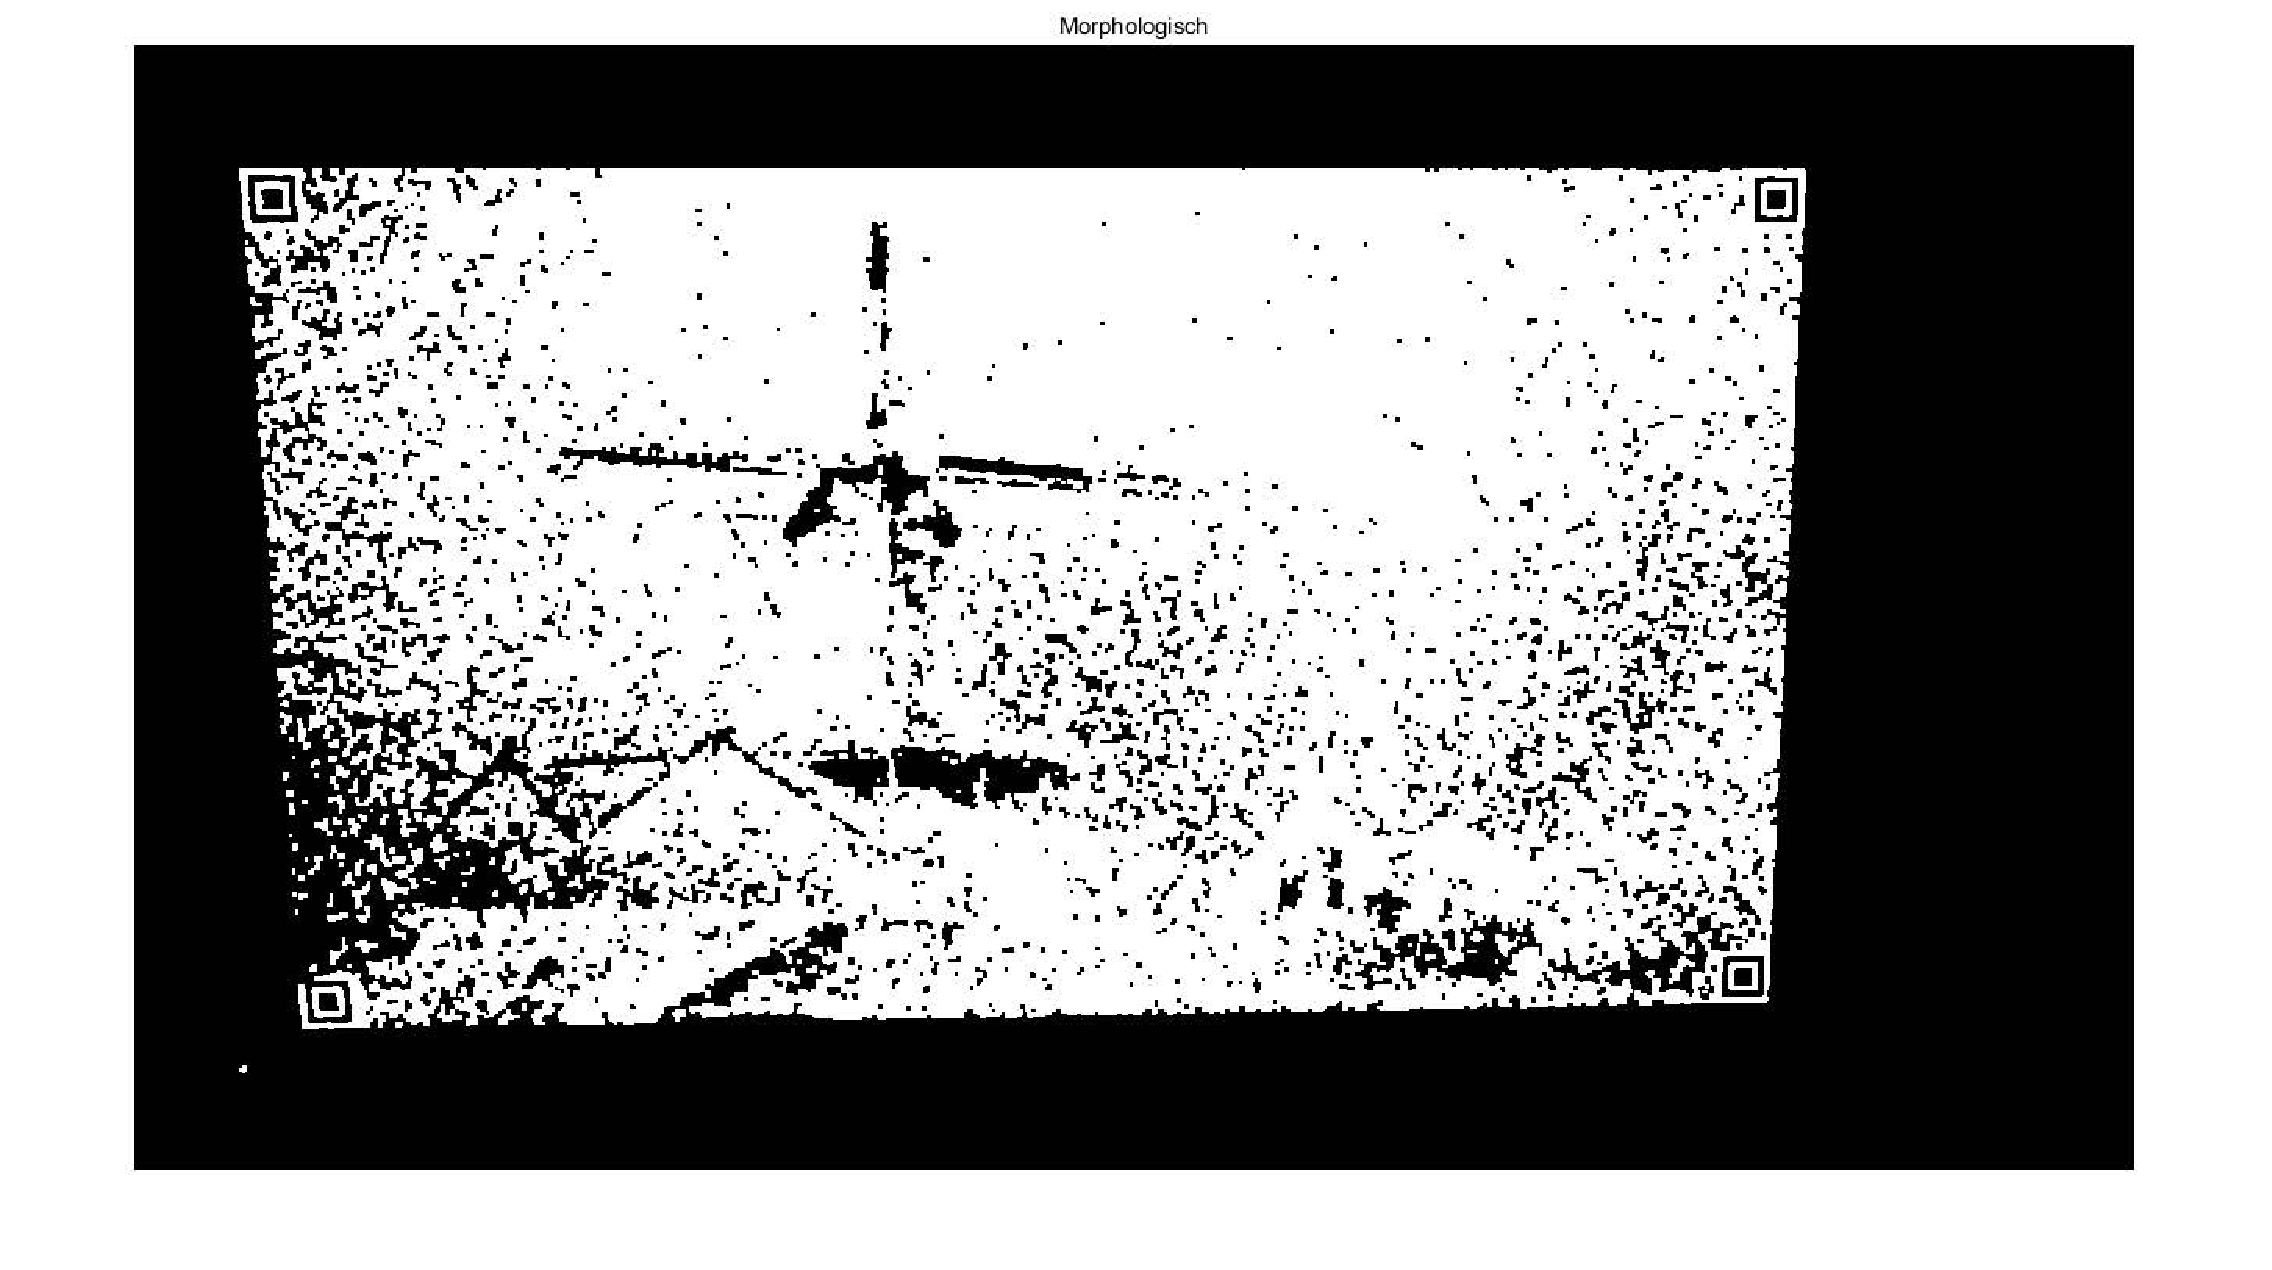
\includegraphics[width=1.0\textwidth]{images/5_Implementirung/morpho.pdf}
\caption{Morphologisch}
\label{fig:morpho}
\end{minipage}
\end{figure}

\begin{figure}[H]
\centering 
\begin{minipage}[b]{0.49\textwidth} 
\centering 
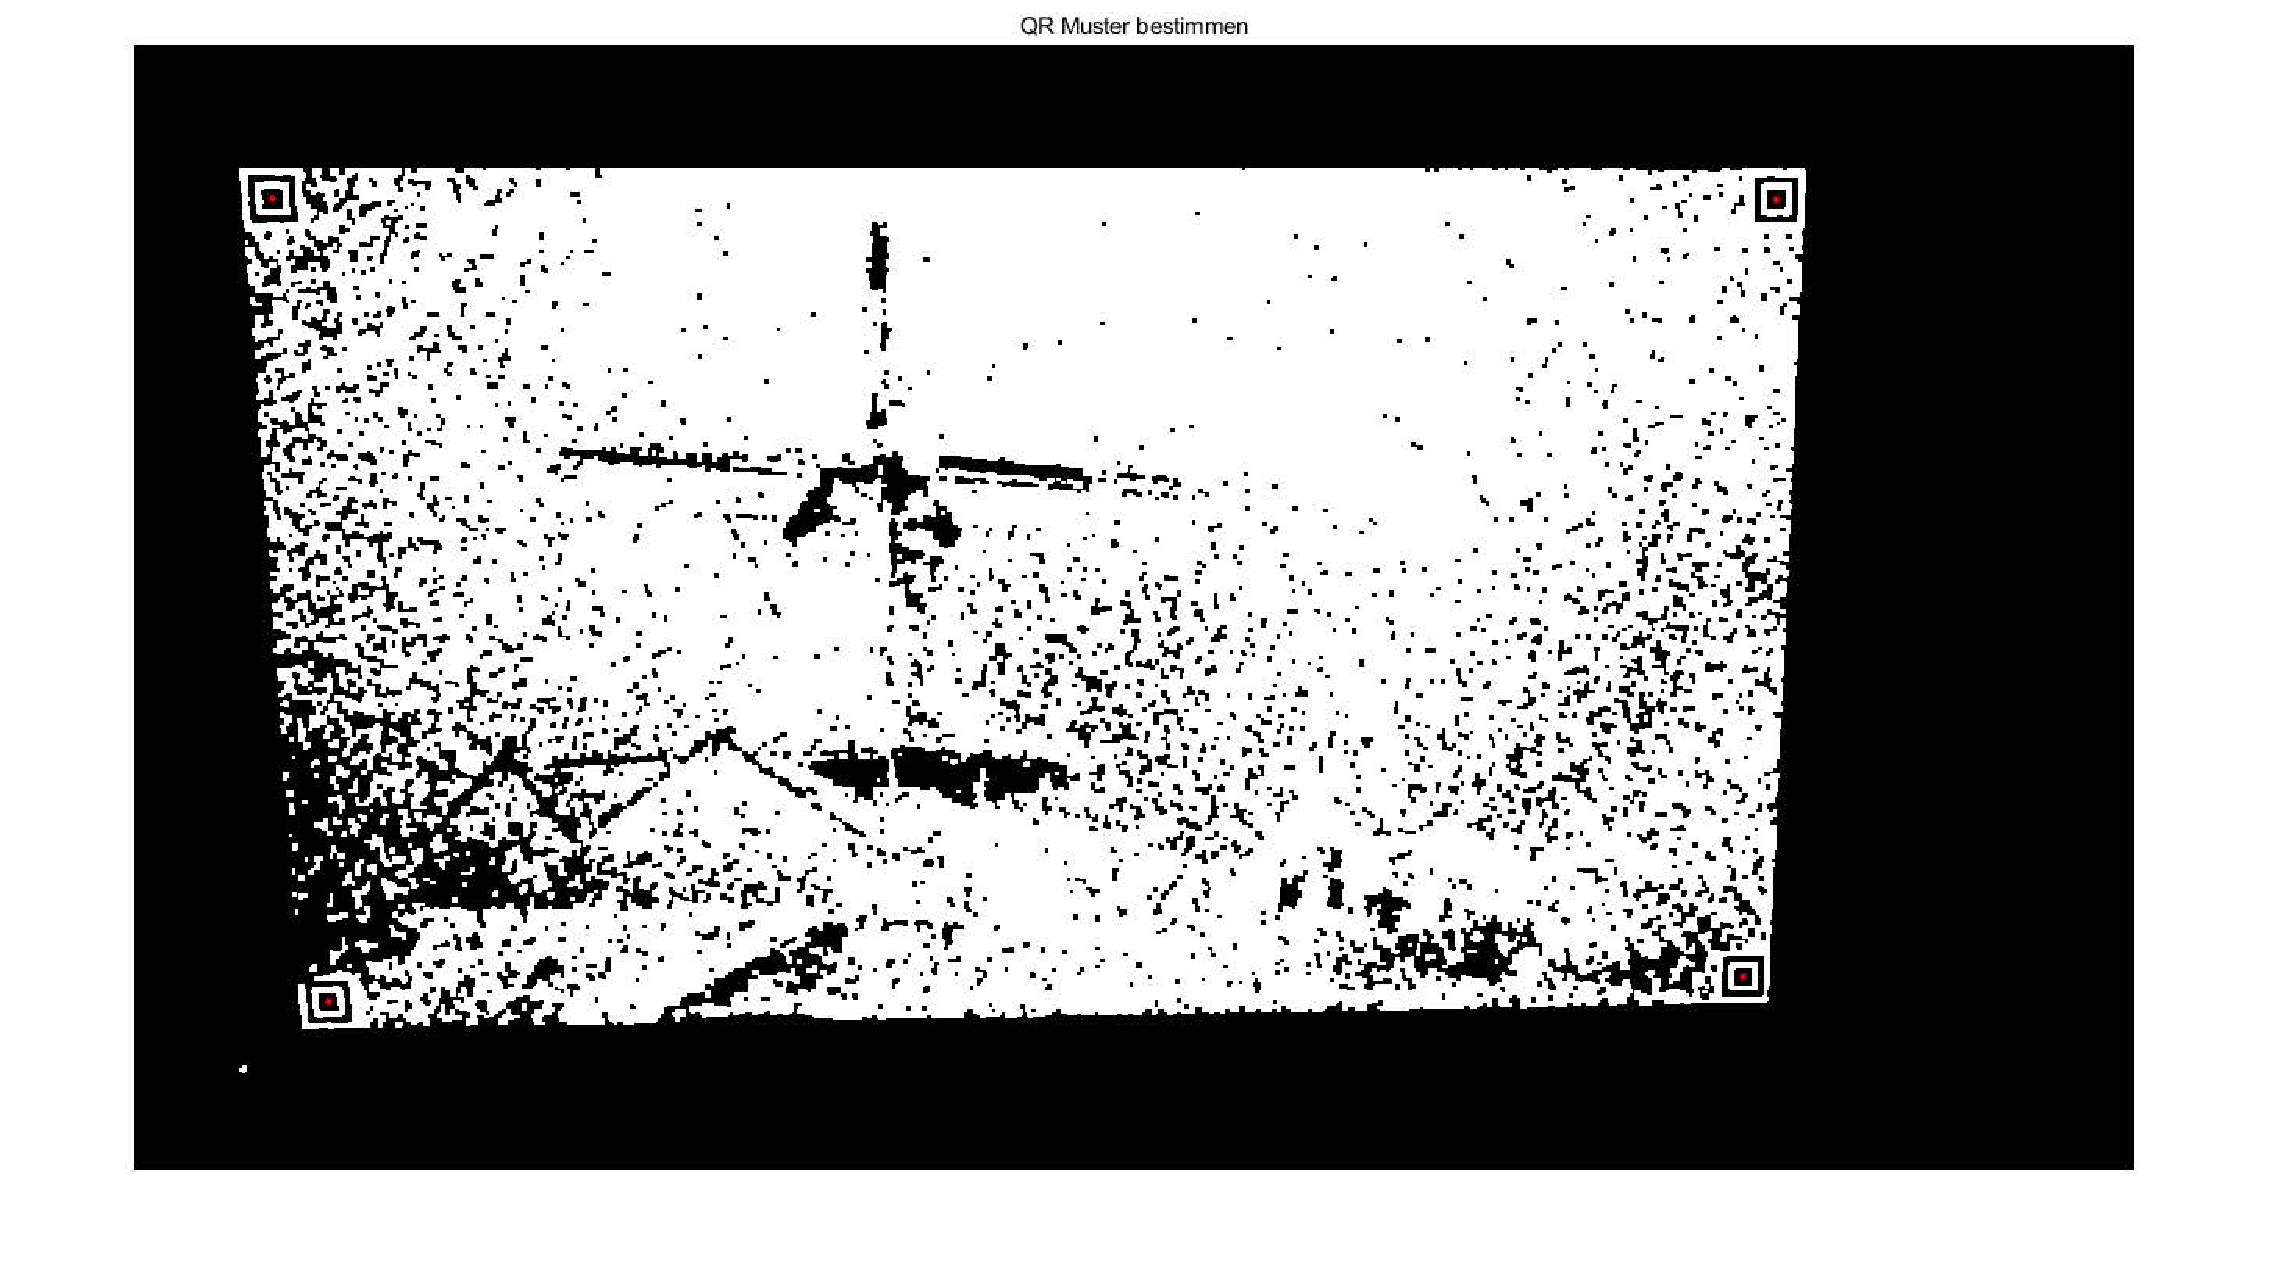
\includegraphics[width=1.0\textwidth]{images/5_Implementirung/QR_muster.pdf} 
\caption{QR Muster}
\label{fig:QR_muster}
\end{minipage}
\begin{minipage}[b]{0.49\textwidth} 
\centering 
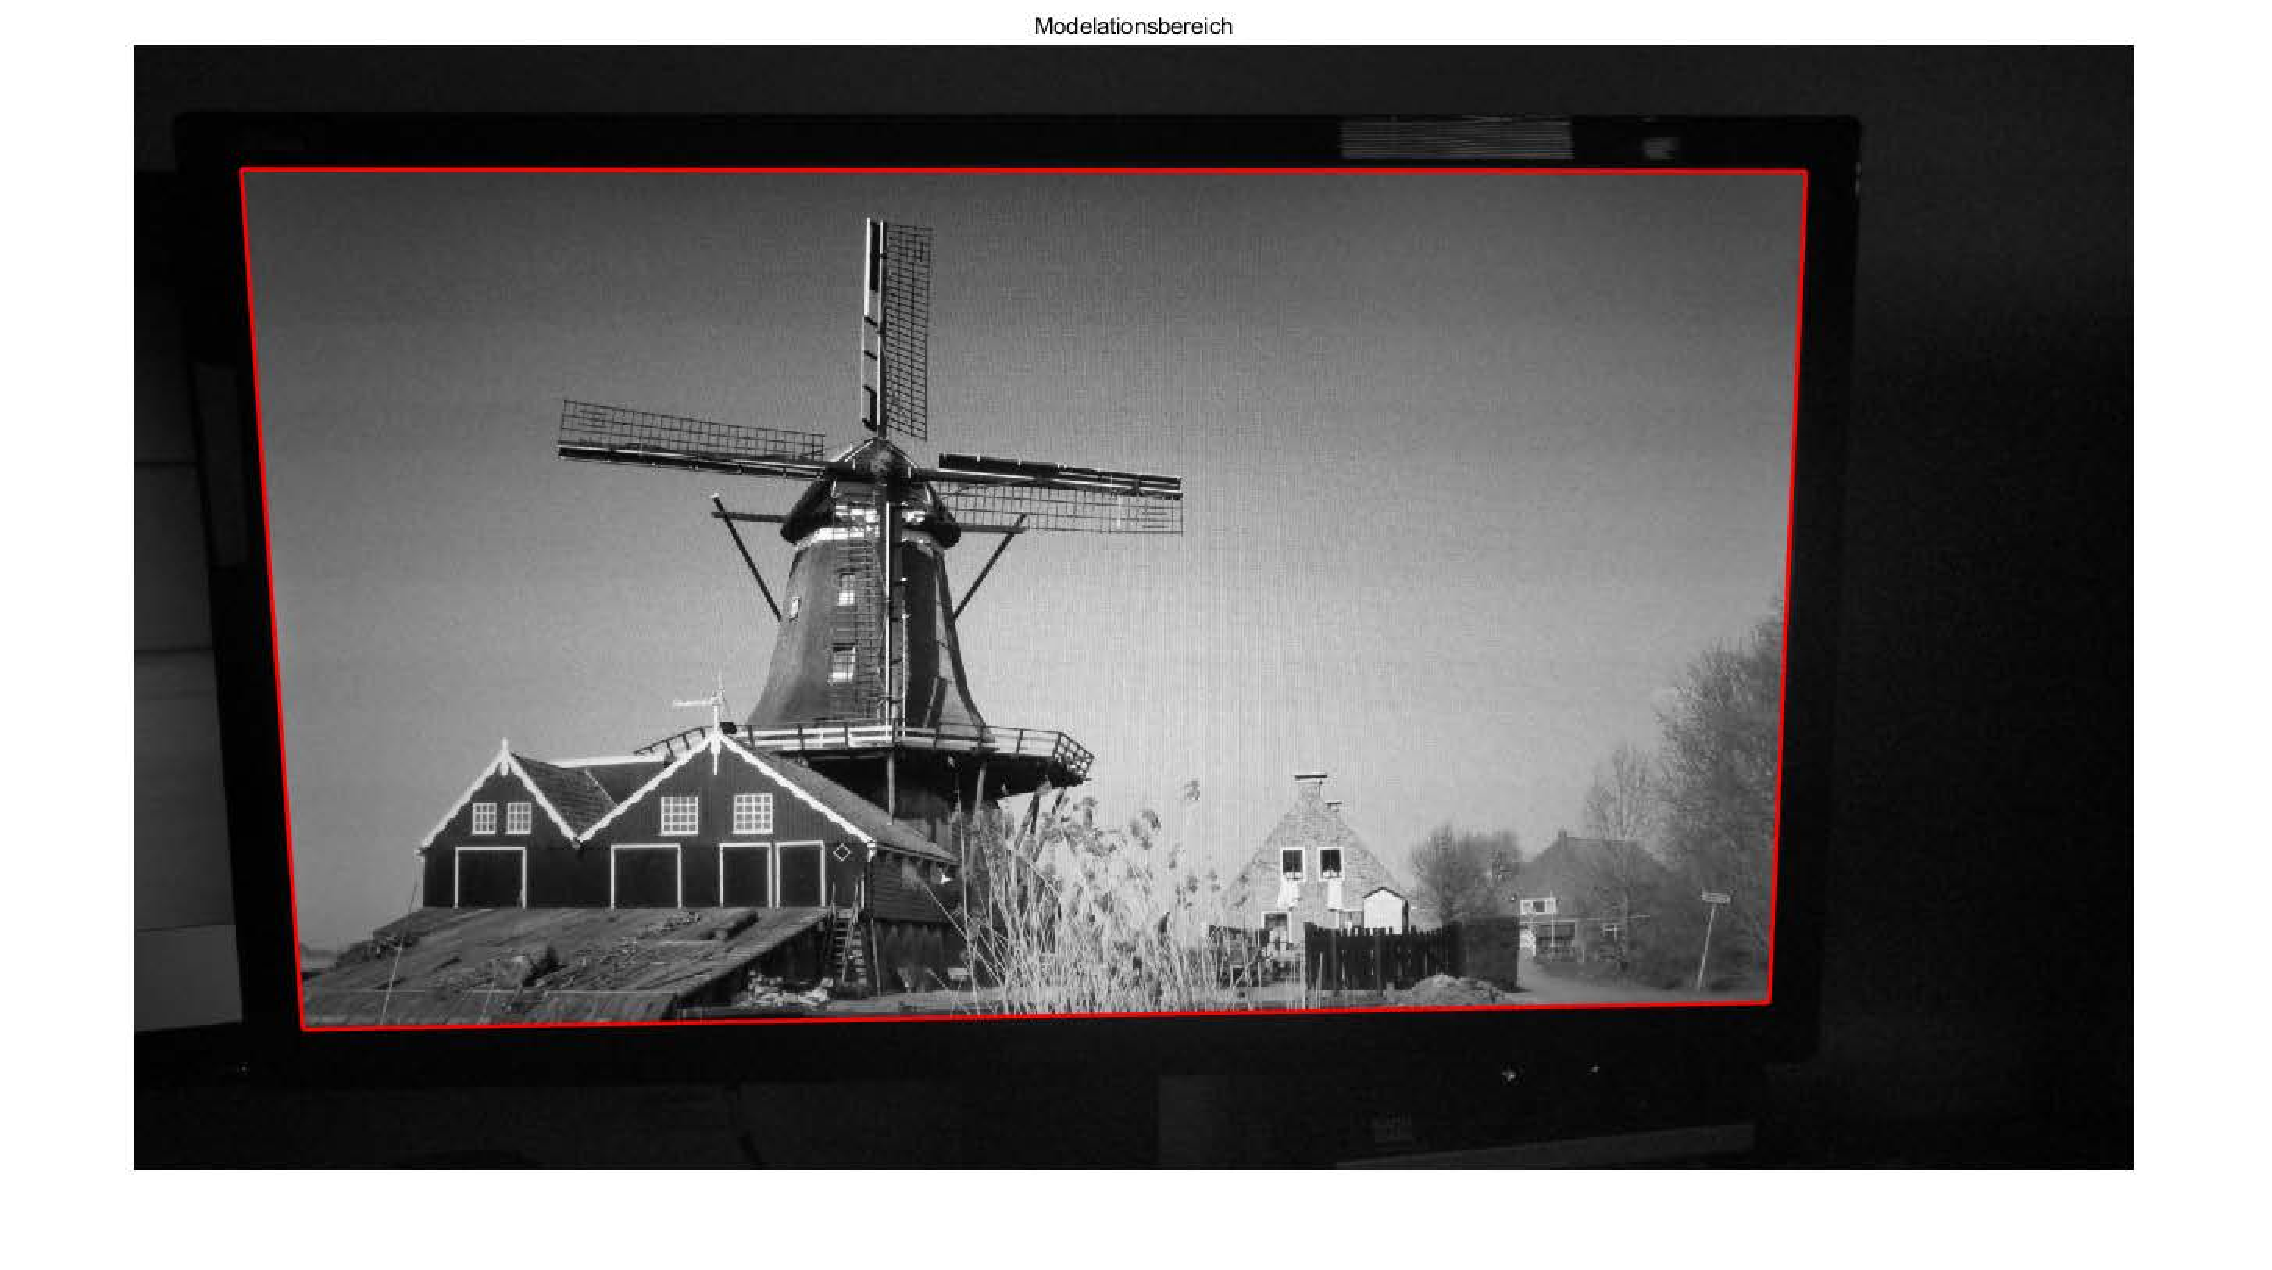
\includegraphics[width=1.0\textwidth]{images/5_Implementirung/Mudulaition.pdf}
\caption{Mudulaitionsbereich}
\label{fig:Mudulaitionbereich}
\end{minipage}
\end{figure}

\begin{figure}[H]
 \centering 
  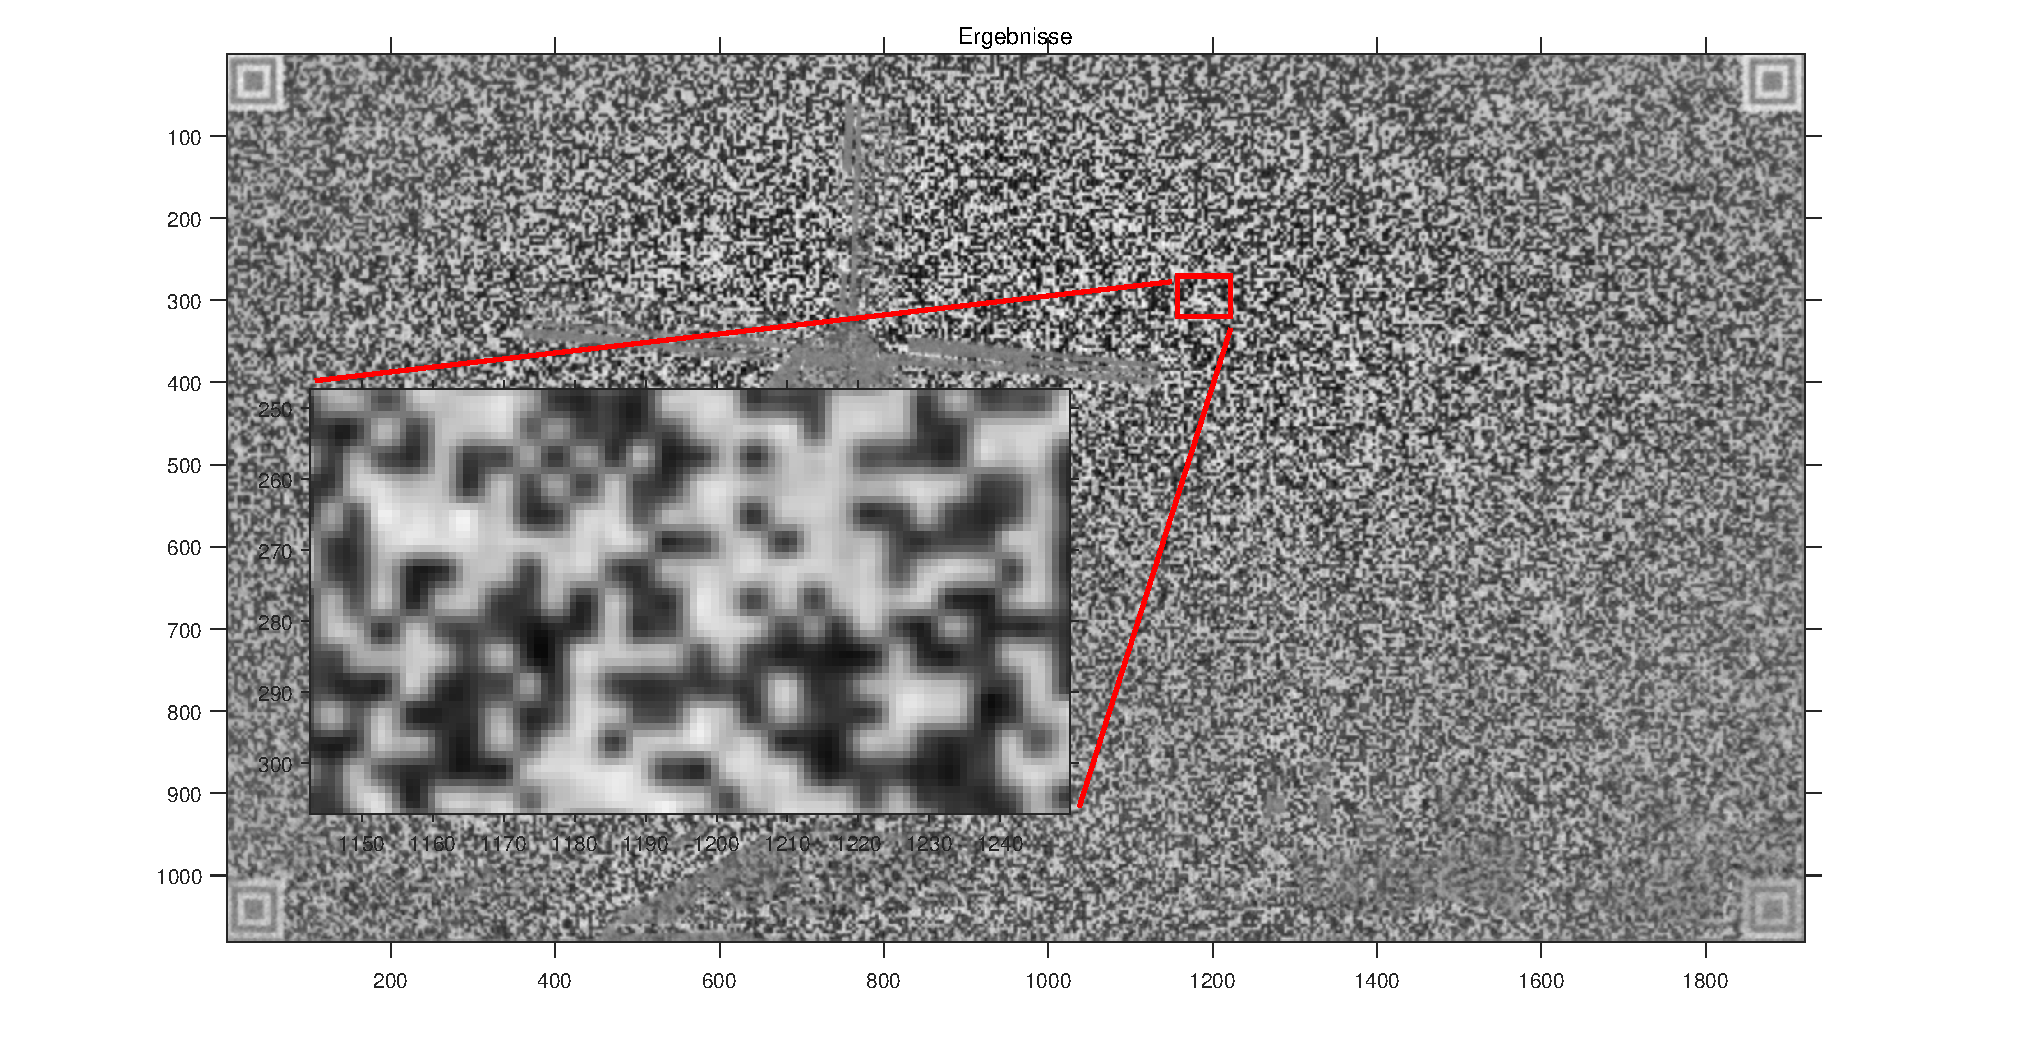
\includegraphics[keepaspectratio,width=0.85\textwidth]{images/5_Implementirung/diffq8.eps}
 \caption{Modulationsbereich im U-Kanal}
 \label{fig:Ergebnis1}
\end{figure}

%\begin{figure}[H]
% \centering 
%  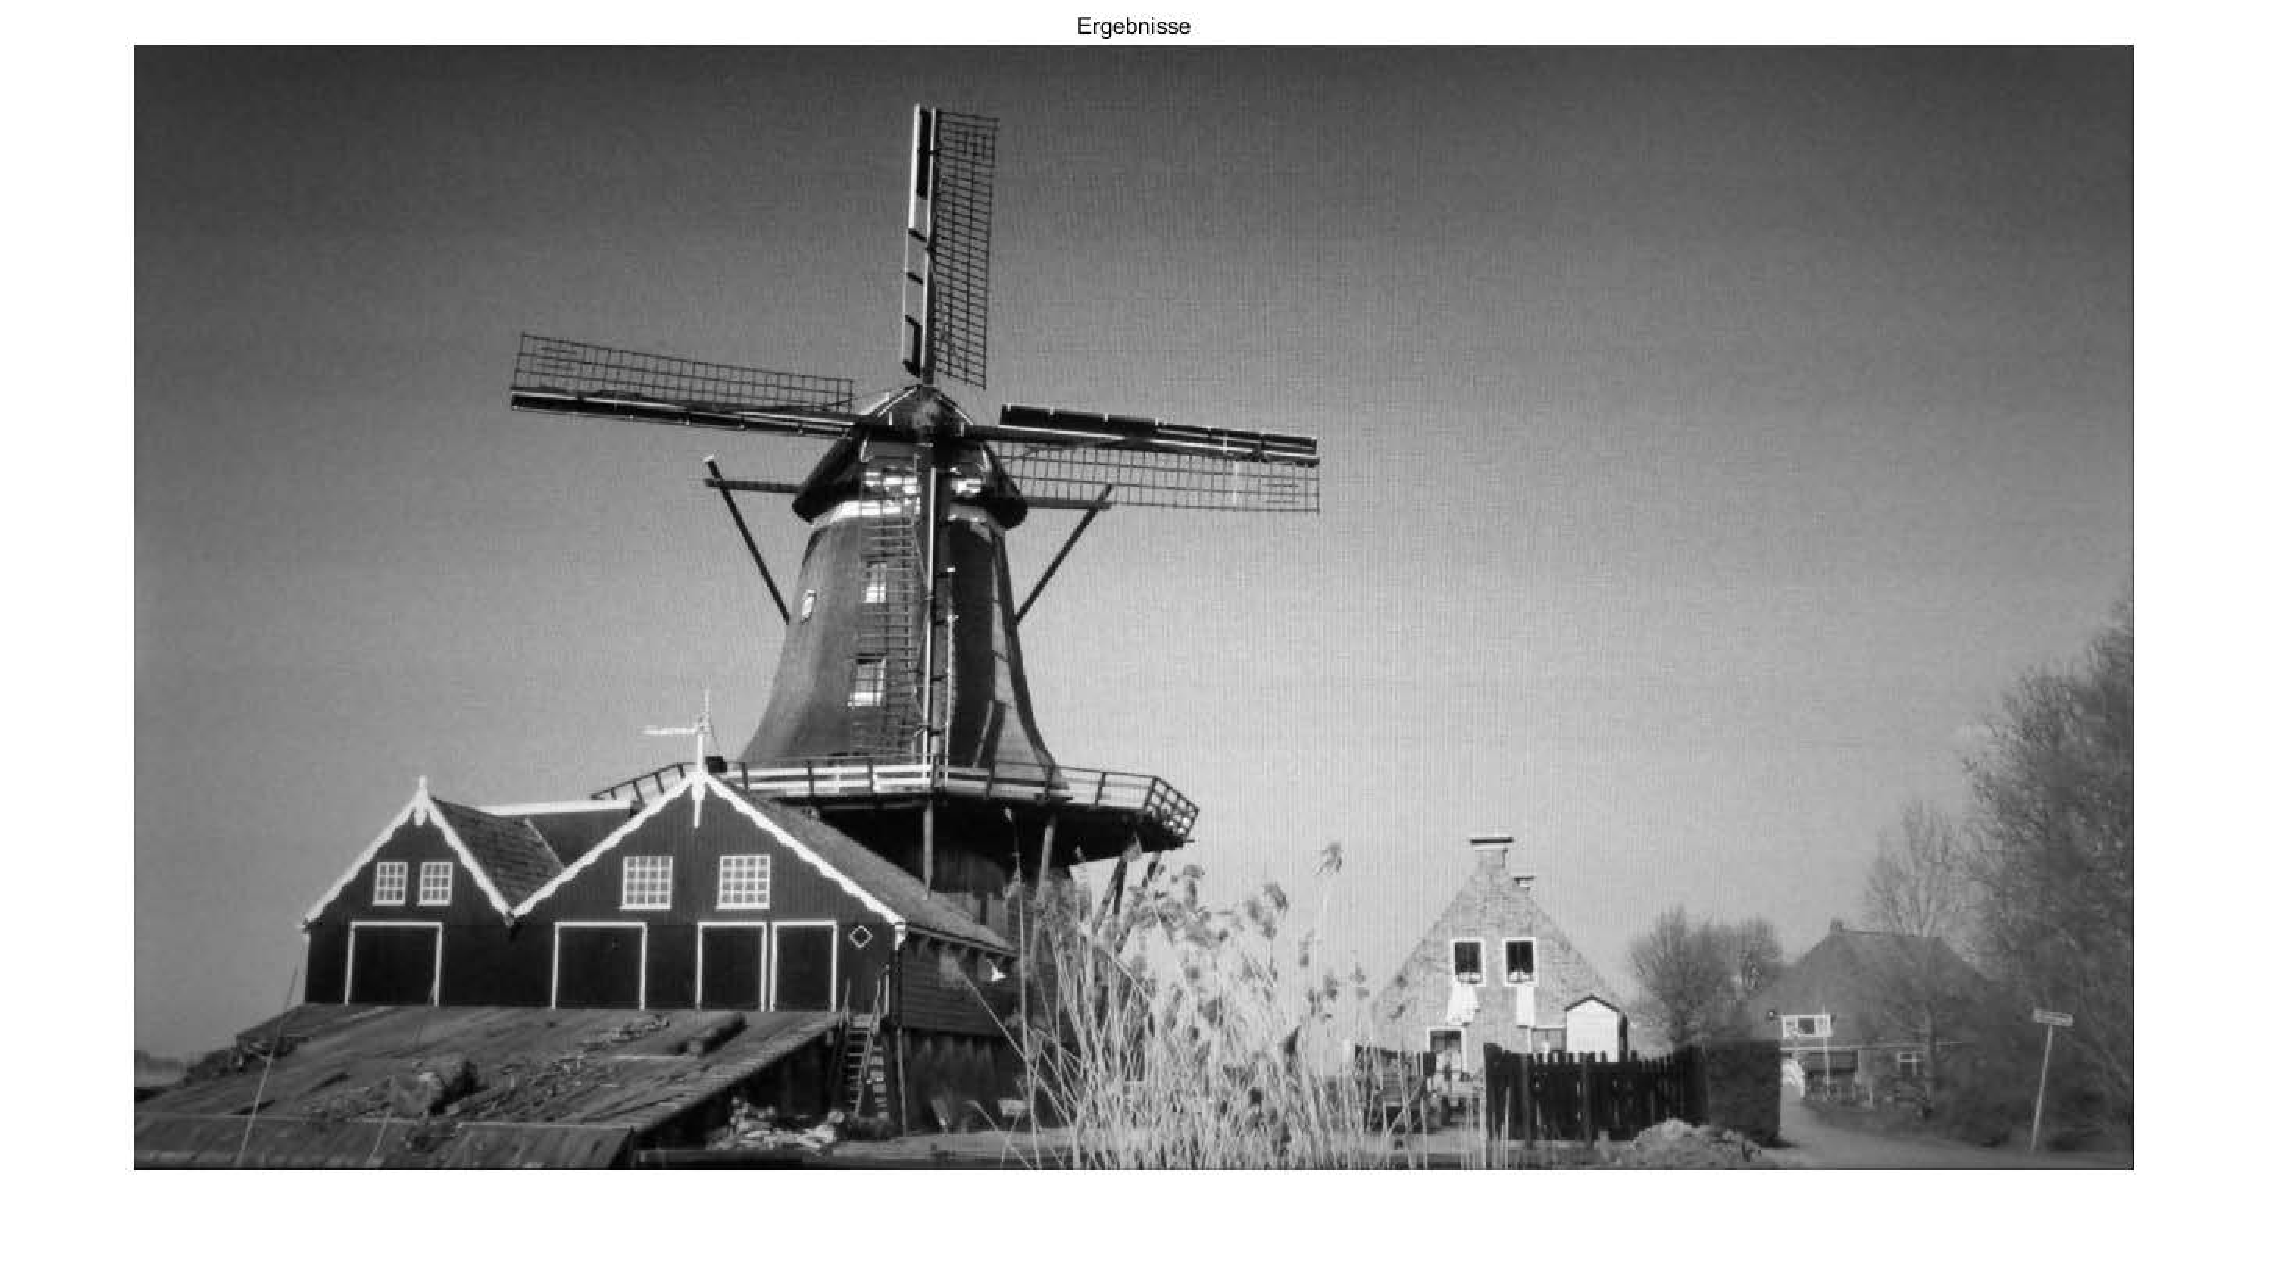
\includegraphics[keepaspectratio,width=1.0\textwidth]{images/5_Implementirung/ergeb.pdf}
% \caption{Ergebnis der 1. Methode}
% \label{fig:Ergebnis1}
%\end{figure}

%Als Nächst einige Ergebnisse der Verwendungen von die 1. Methode wird angegeben.



\section{Implementierung vom zweiten Verfahren}

Hier wird die Implementierung der zweiten Methode vorgestellt. Das Bild stammt aus einer Reihe von acht Bildern, die durch ein Google Pixel mit Stativ aufgenommen wurden. In dieser Situation wird keine Bildregistrierung verwendet. Dies bedeutet, dass sich der Inhalt des Videos verändern lässt. Die Modulationsamplitude werden hier auf 6 und der Daten Datenblock auf $ 4 \times 4 Pixel$ eingestellt. 

Durch das Wissen des 4. Kapitels, werden von diesen Bildern eine Reihe Differenzbilder erstellt. Die 3 Differenzbilder mit der größten $``Energie"$ werden addiert, um ein zu detektierendes Bild zu erhalten, wie in Abbildung \ref{fig:diff2} zu sehen ist. Anschließend wird unter Verwendung der Binarisierungmethode, Ostu Schwellenmethode, ein Binärbild generiert, indem der Modulationsbereich des Bildes extrahiert wird. Um kleine Punkte und Lücken zu beseitigen, lässt sich eine Morphologie Operation durchführen. Das hier benutzte Strukturelement ist ein $5 \times 5$ Quadrat. Die Wirkungen beider Operationen werden in Abbildung \ref{fig:binar2} und Abbildung \ref{fig:morph2} gezeigt. Um der Einfluss der Kamera-Verzerrung zu neutralisieren, wird das Binärbild mit einer Cross Dilatation verarbeitet, also $ n_{around} = 1$. Struktur der Cross Dilatation wird in Abbildung gezeigt und Abbildung \ref{fig:cd} zeigt diese Operation. 
In der Radon Transformation lässt sich das Bildzentrum auf den Ursprung setzen. Dann durch Vergleich der Integralwerte kann die längste Linie, welche die oben, unten, links und rechts liegt, gefunden werden. Um die Berechnungskosten zu reduzieren, werden nur die Linien innerhalb von $ \pm 10^{\circ} $ erkannt. 
\begin{figure}[H]
\centering 
\begin{minipage}[b]{0.49\textwidth} 
\centering 
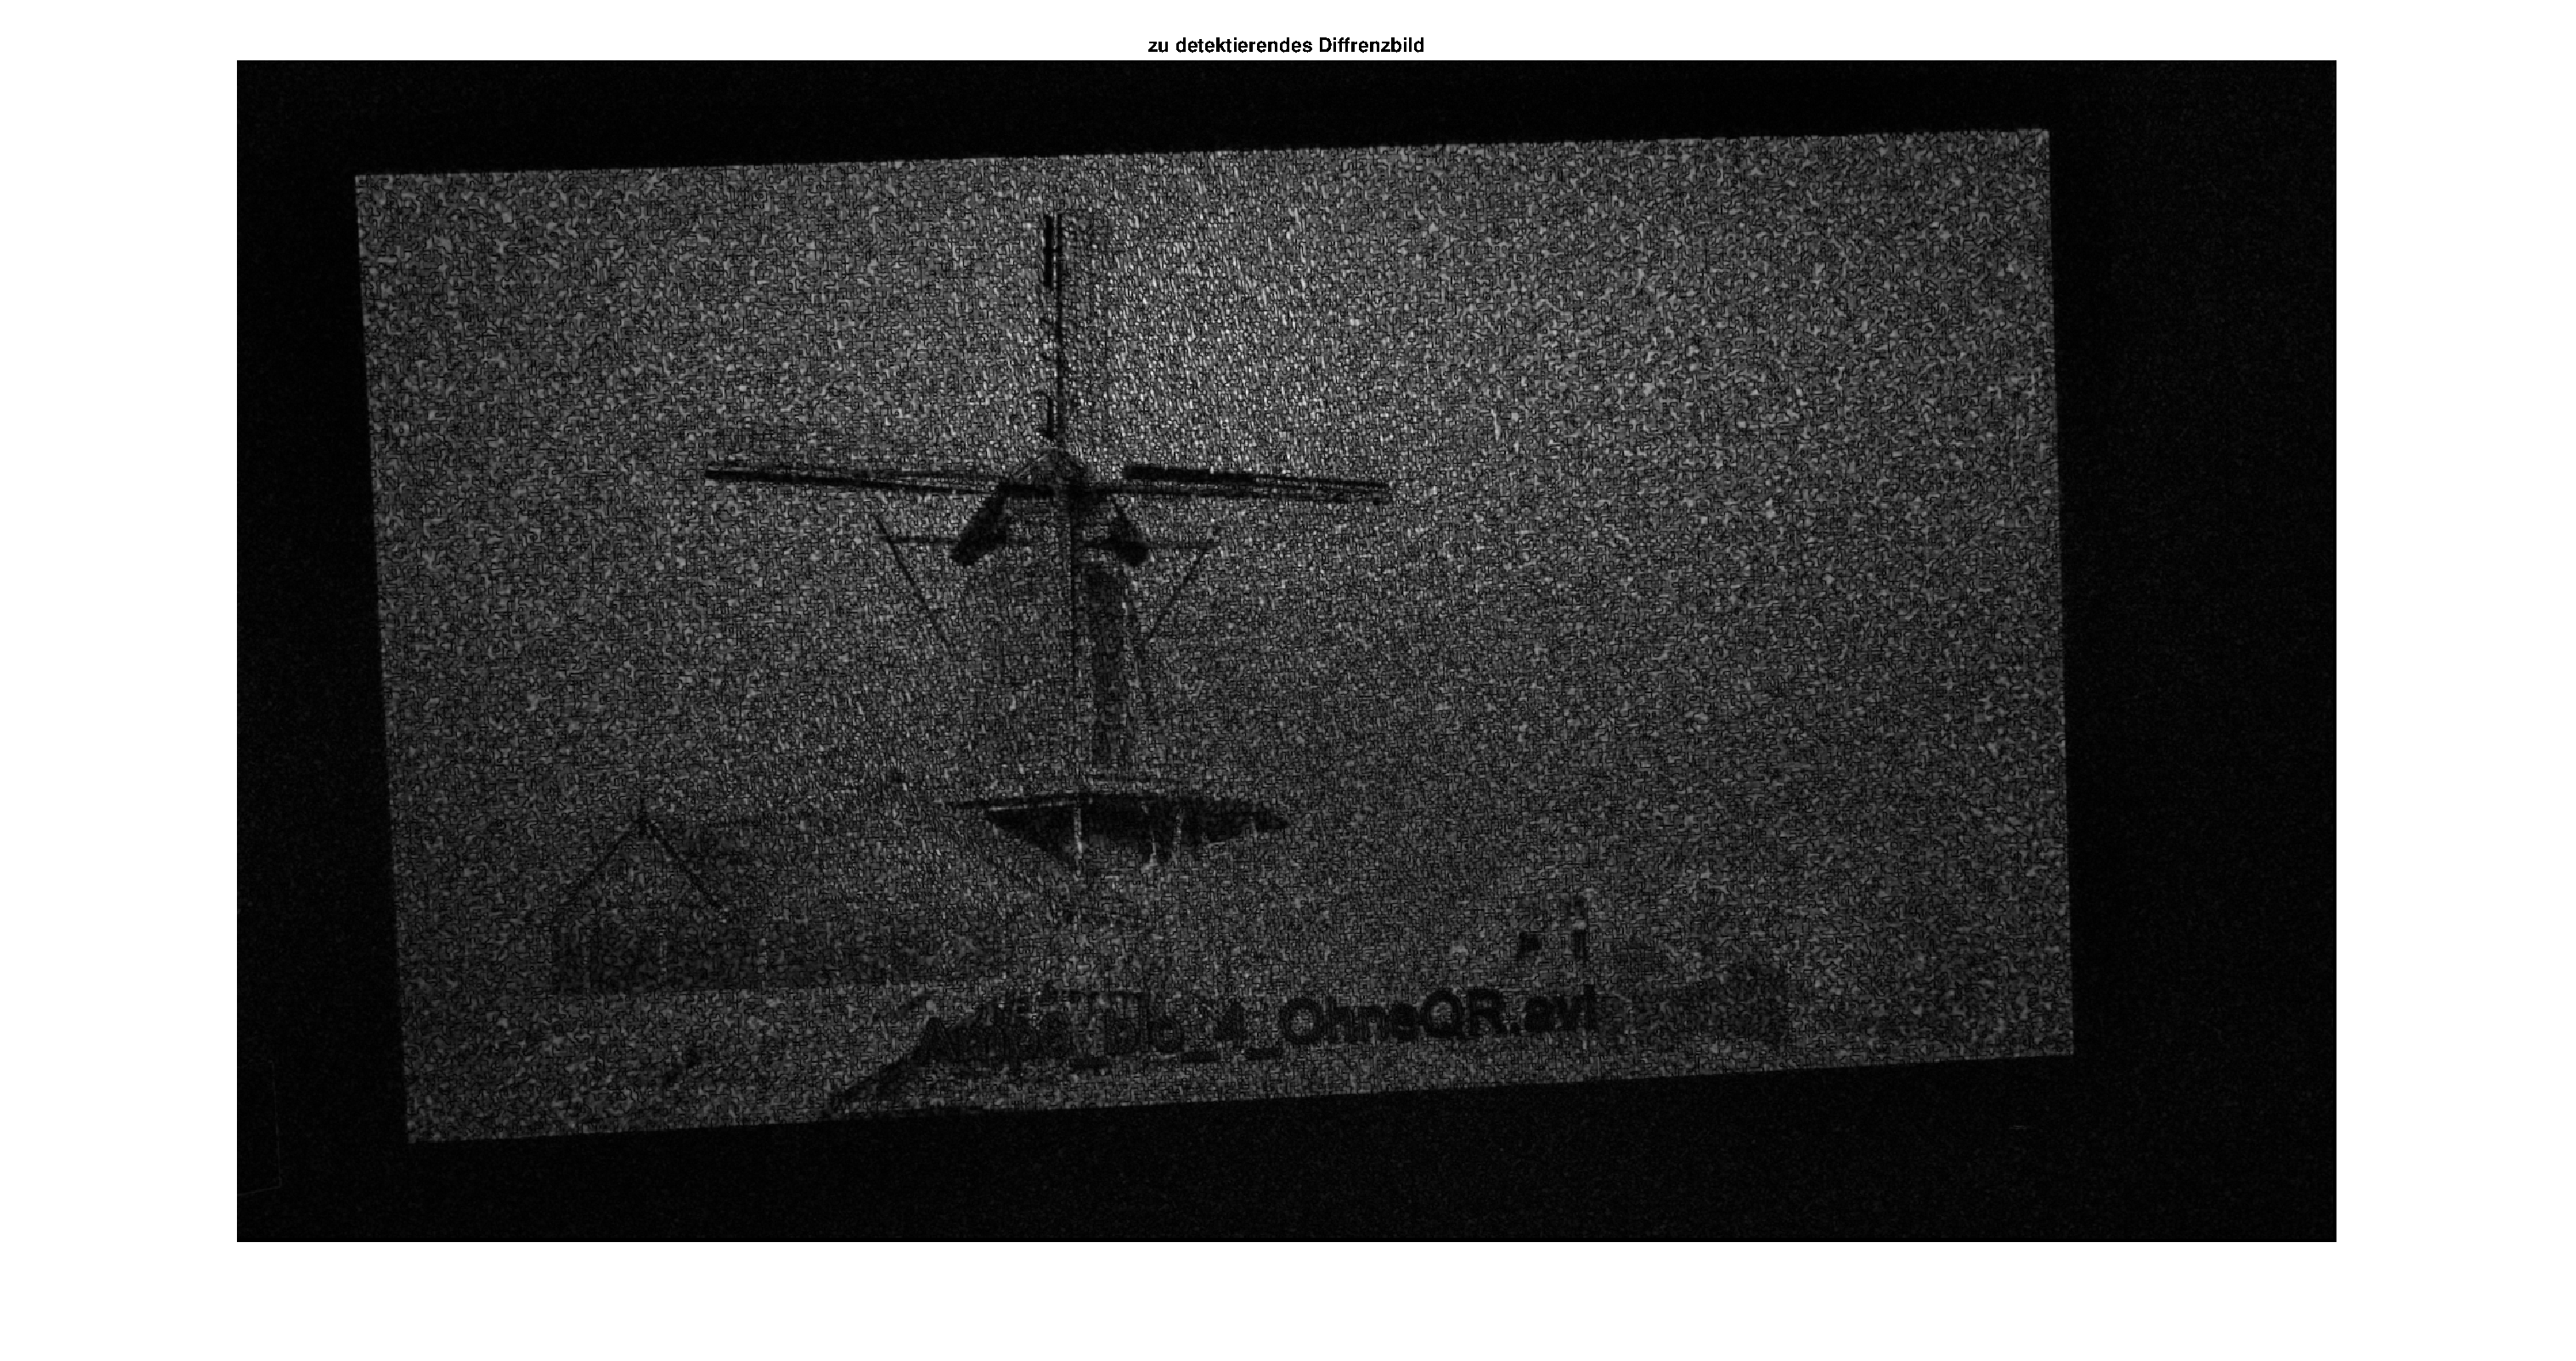
\includegraphics[width=1.06\textwidth]{images/5_Implementirung/2/diff.eps} 
\caption{Ein zu detektierendes Bild}
\label{fig:diff2}
\end{minipage}
\begin{minipage}[b]{0.49\textwidth} 
\centering 
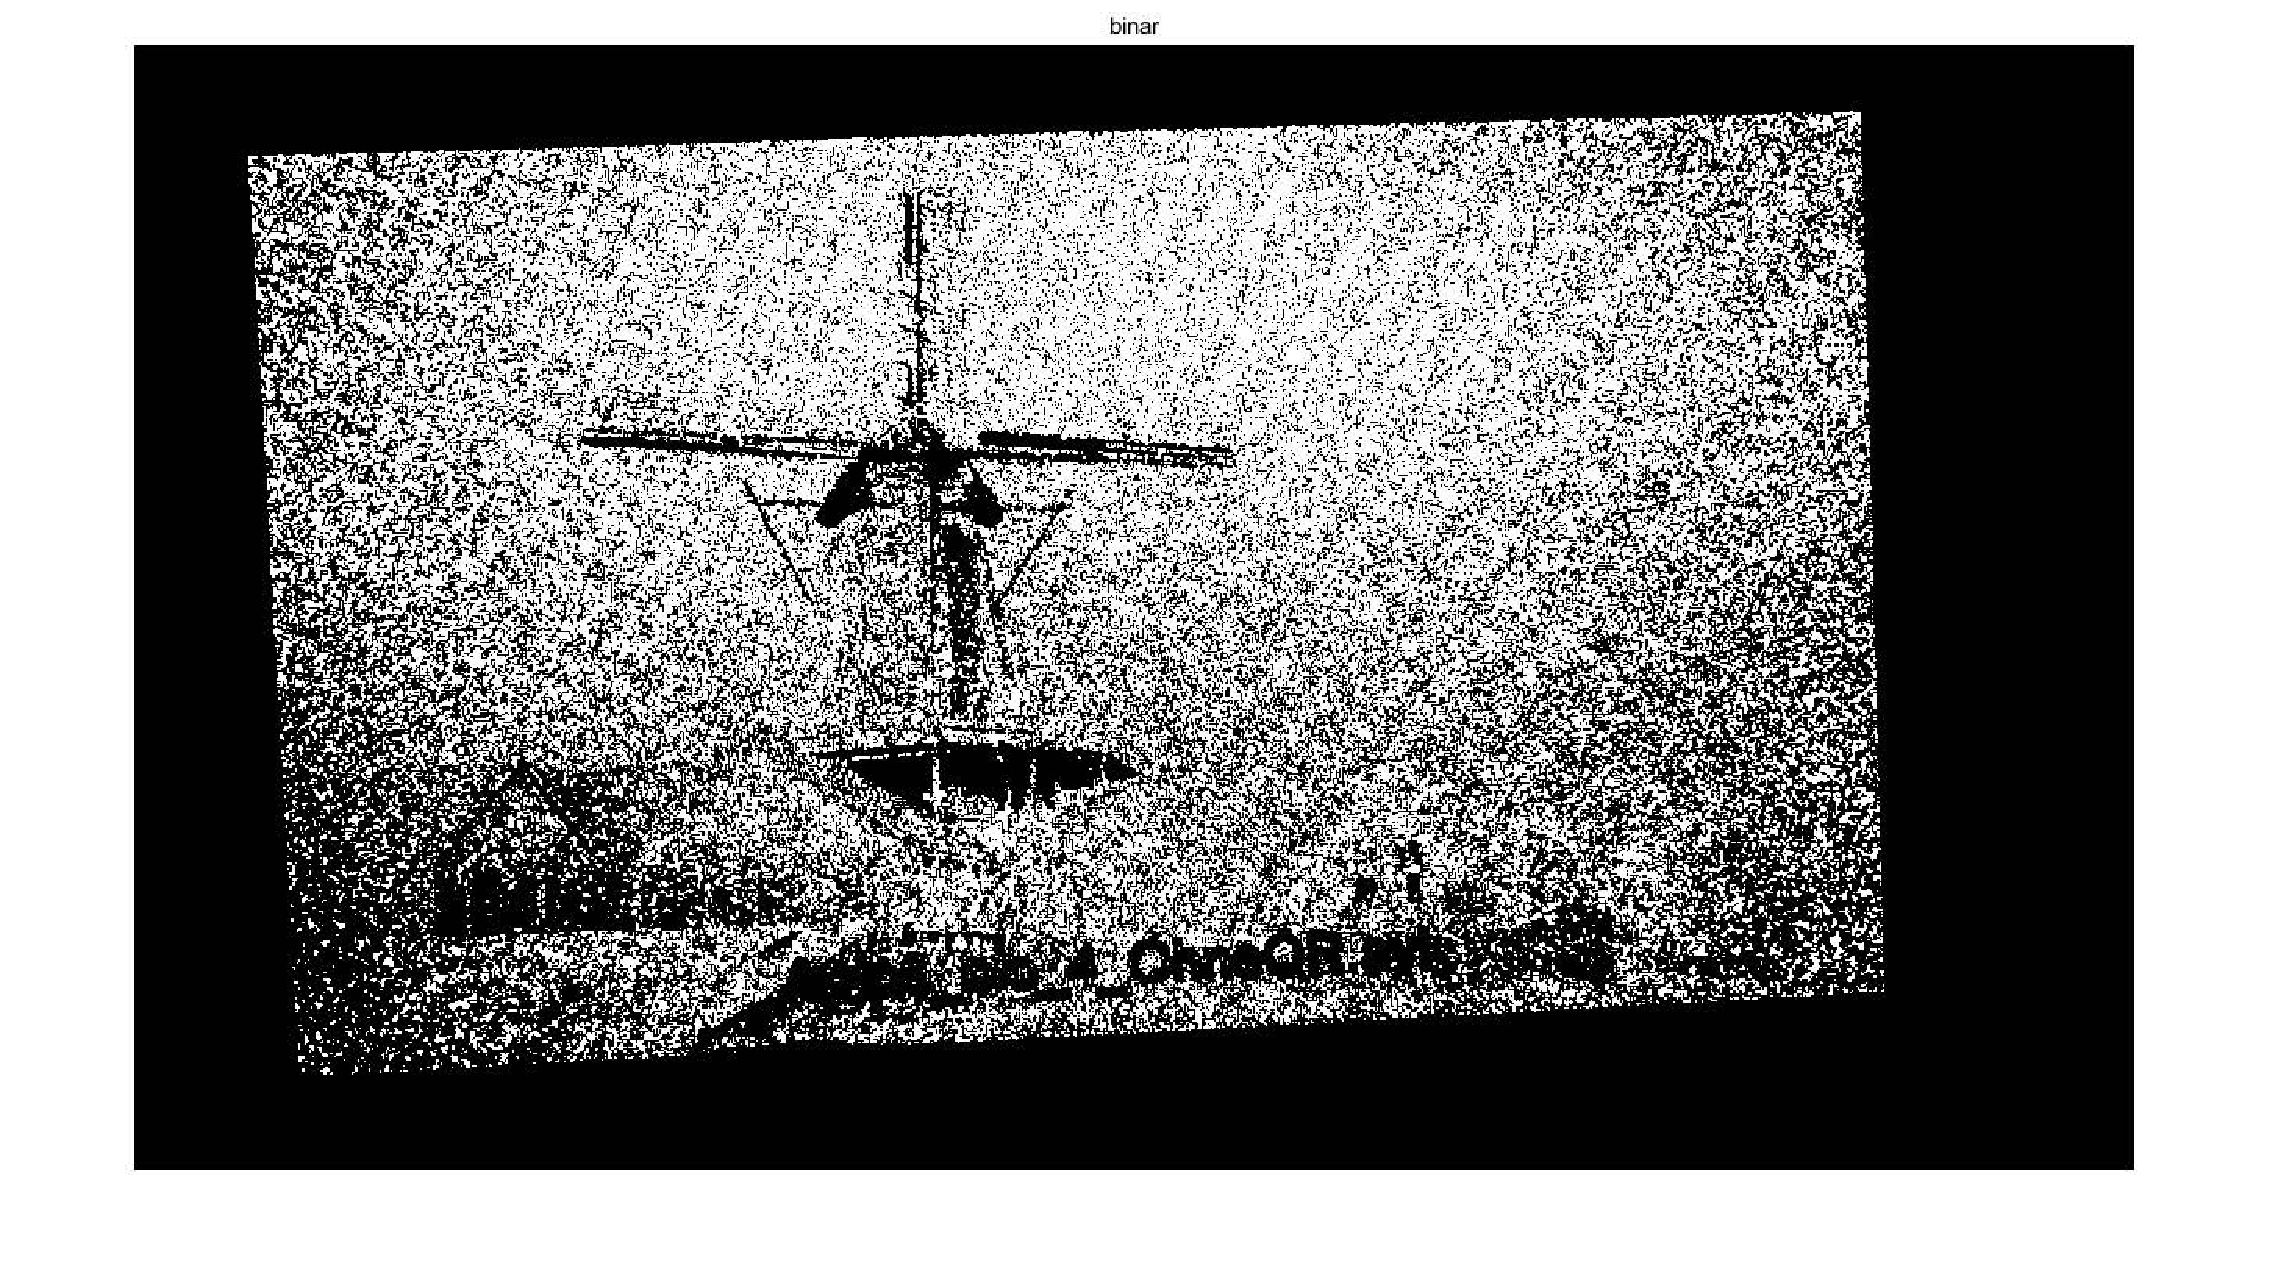
\includegraphics[width=1.0\textwidth]{images/5_Implementirung/2/bina.pdf}
\caption{Binarisierung}
\label{fig:binar2}
\end{minipage}
\end{figure}

\begin{figure}[H]
\centering 
\begin{minipage}[b]{0.49\textwidth} 
\centering 
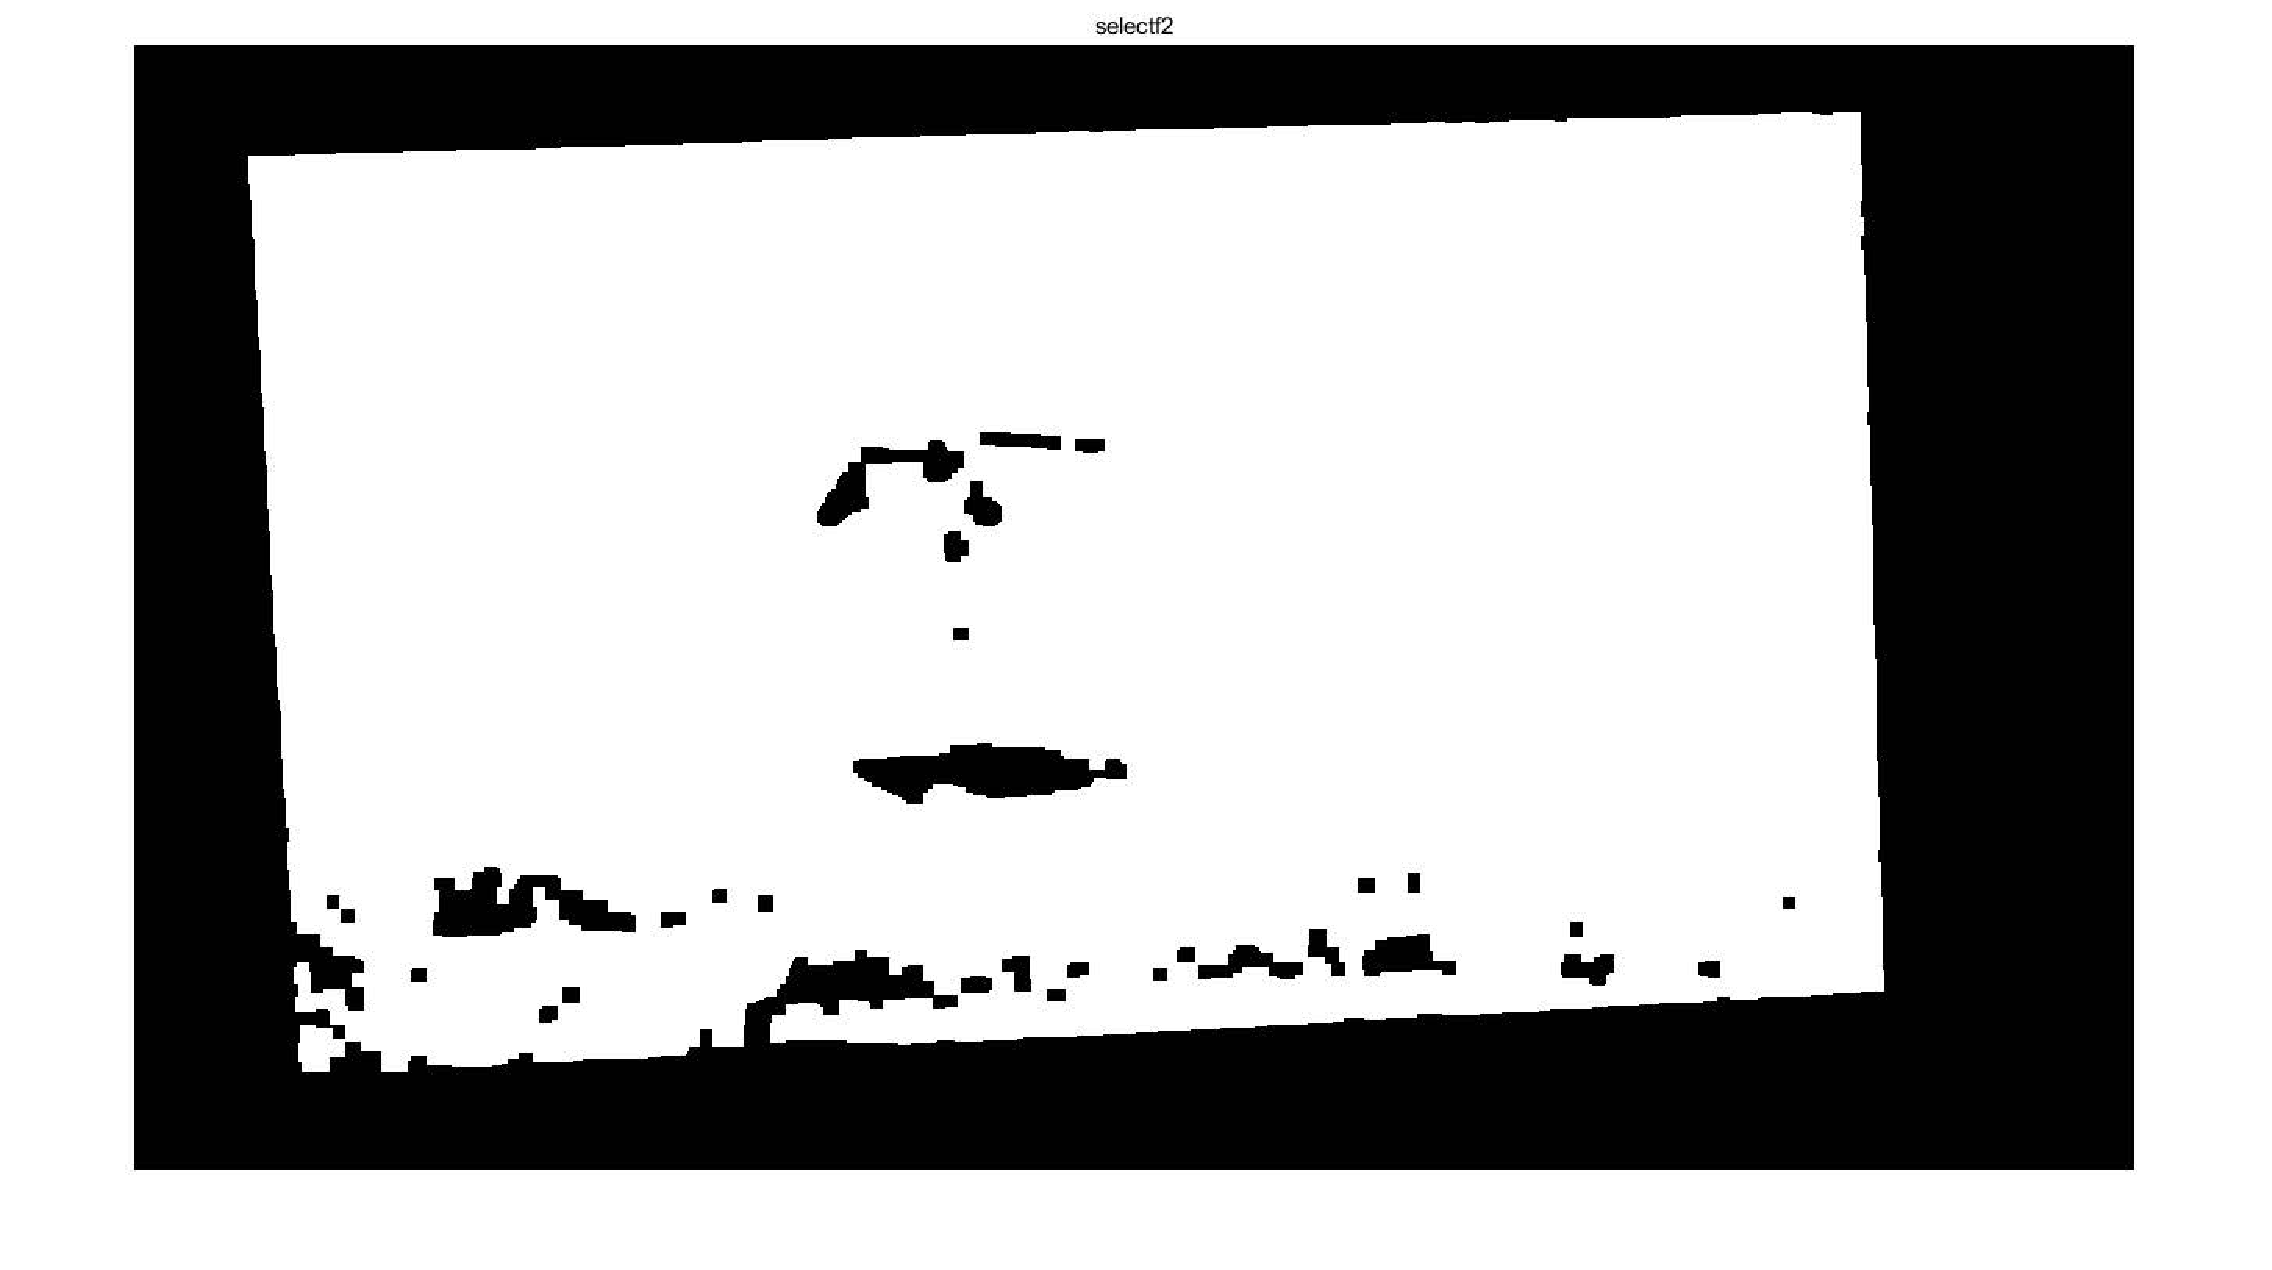
\includegraphics[width=1.0\textwidth]{images/5_Implementirung/2/morpho.pdf} 
\caption{Morphologisch}
\label{fig:morph2}
\end{minipage}
\begin{minipage}[b]{0.49\textwidth} 
\centering 
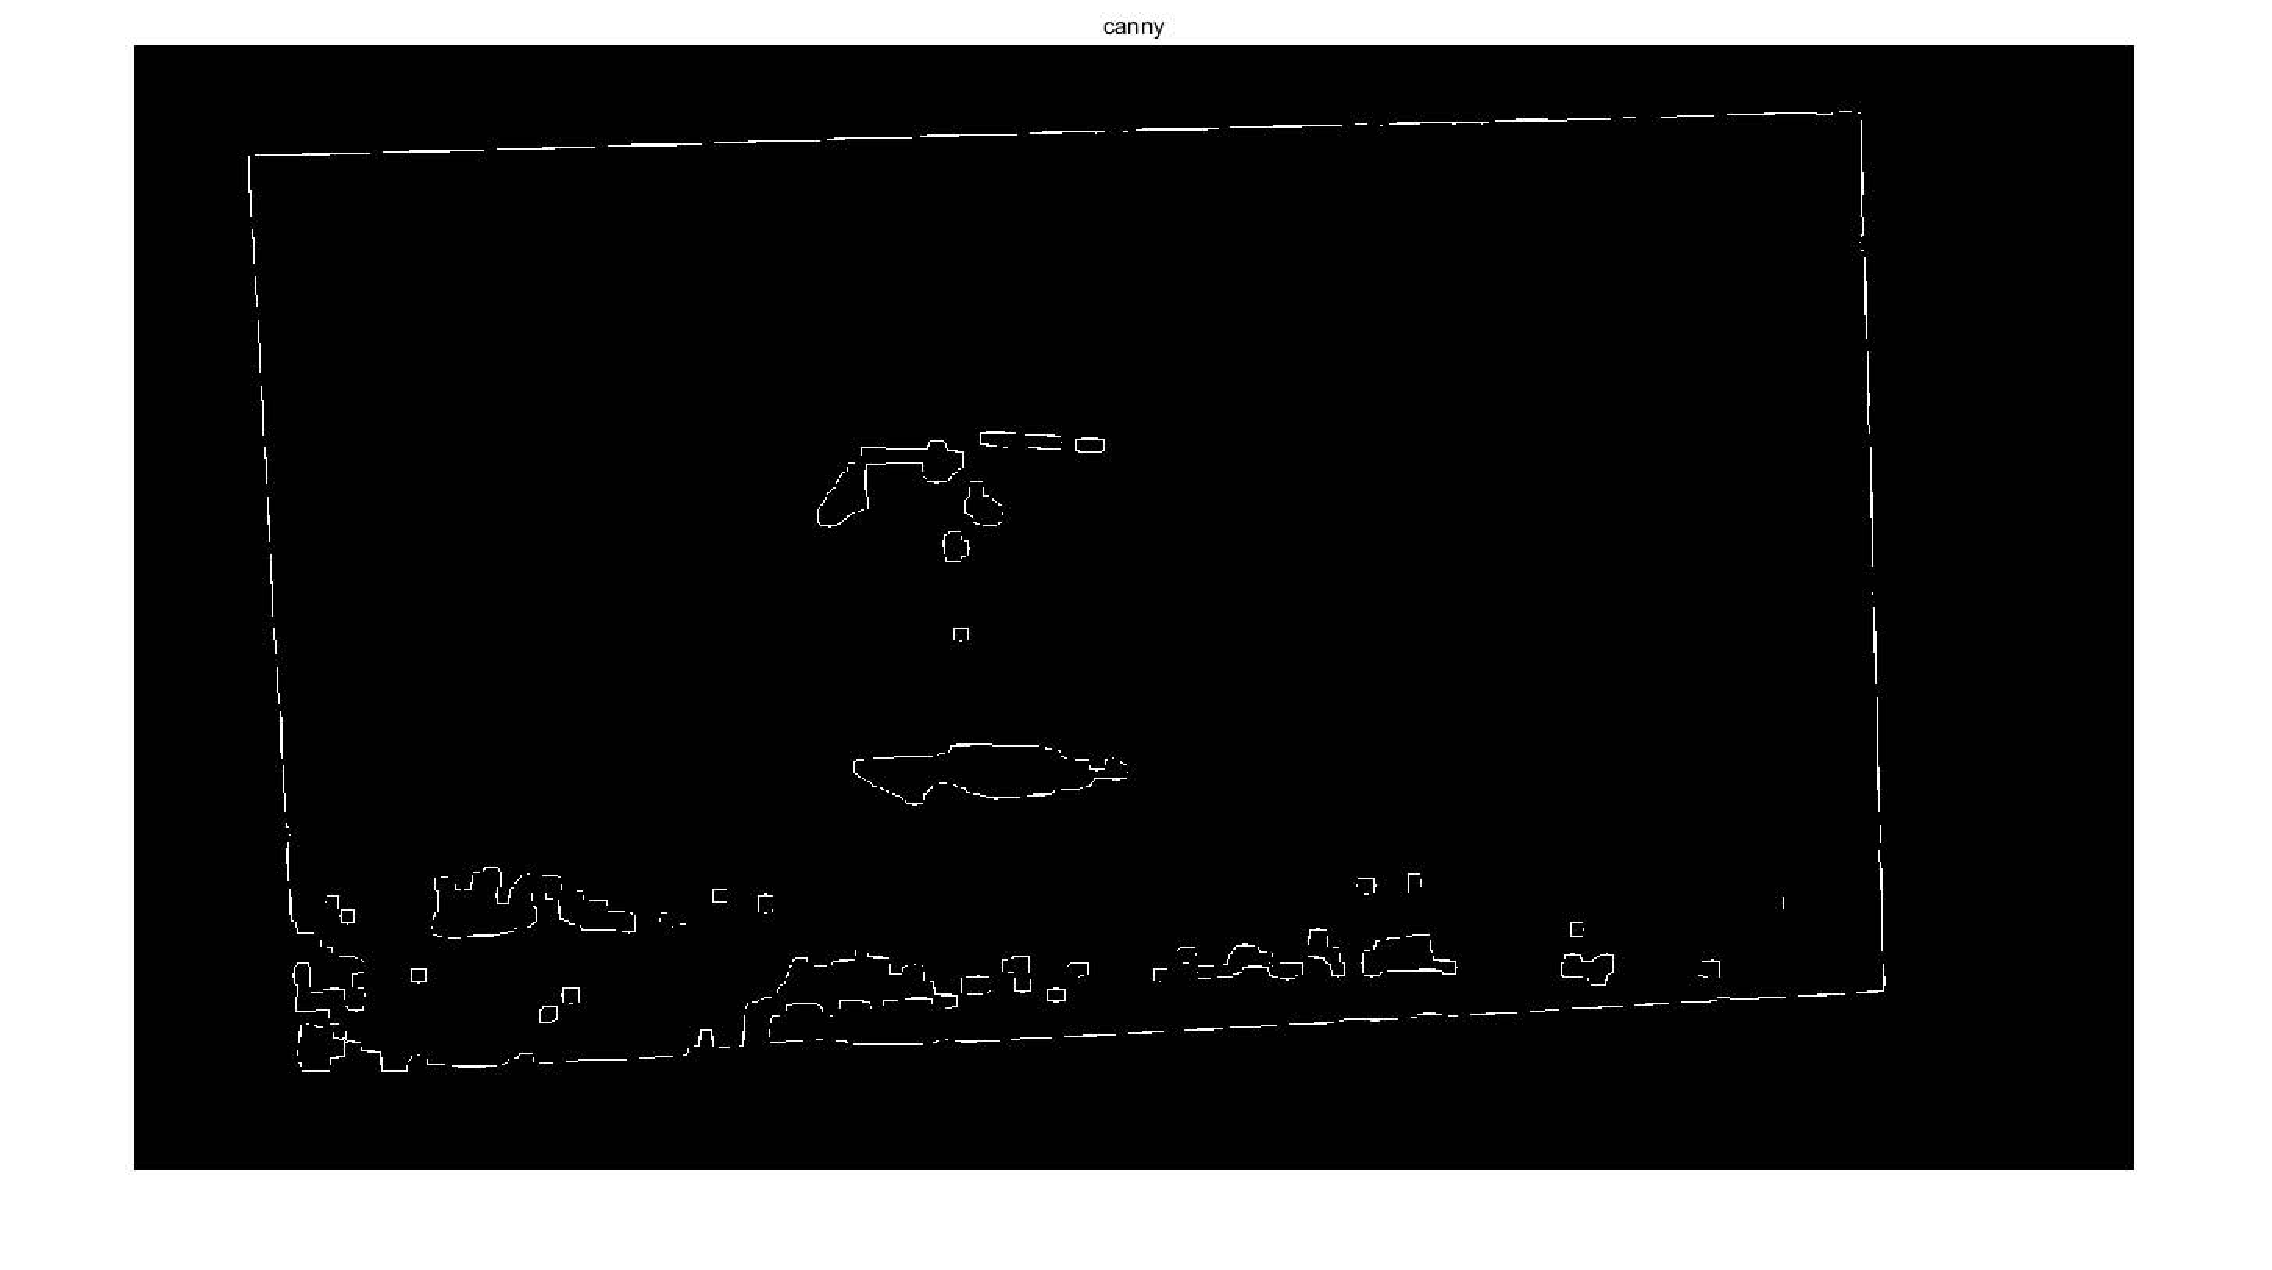
\includegraphics[width=1.0\textwidth]{images/5_Implementirung/2/canny.pdf}
\caption{Canny Detektion}
\label{fig:canny}
\end{minipage}
\end{figure}

\begin{figure}[H]
\centering 
\begin{minipage}[b]{0.49\textwidth} 
\centering 
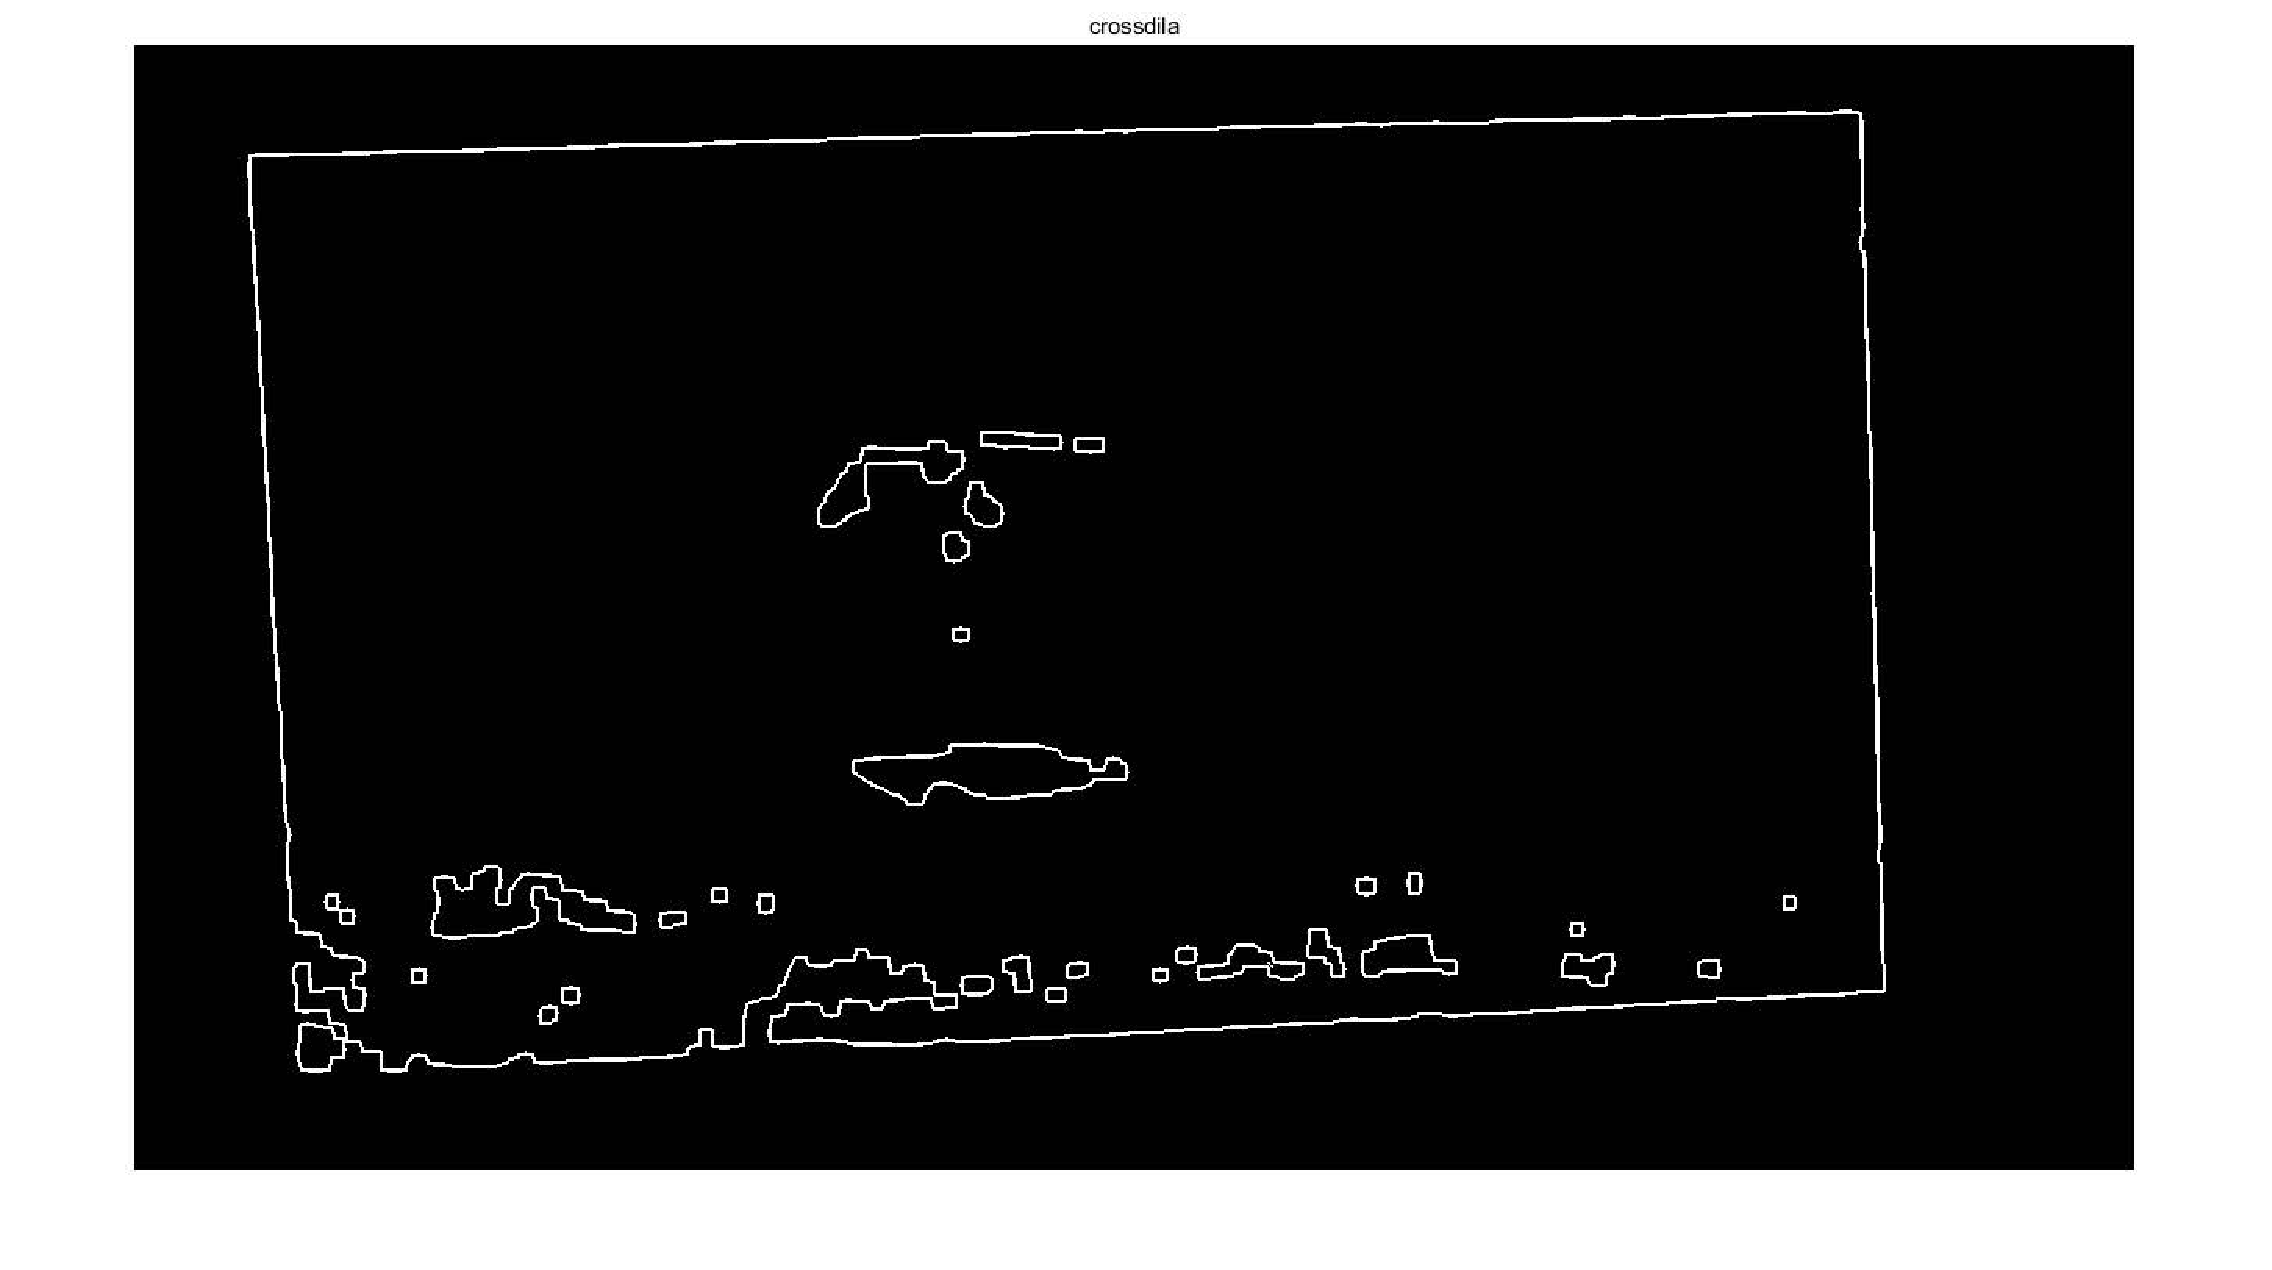
\includegraphics[width=1.0\textwidth]{images/5_Implementirung/2/cd.pdf} 
\caption{Cross Dilatation}
\label{fig:cd}
\end{minipage}
\begin{minipage}[b]{0.49\textwidth} 
\centering 
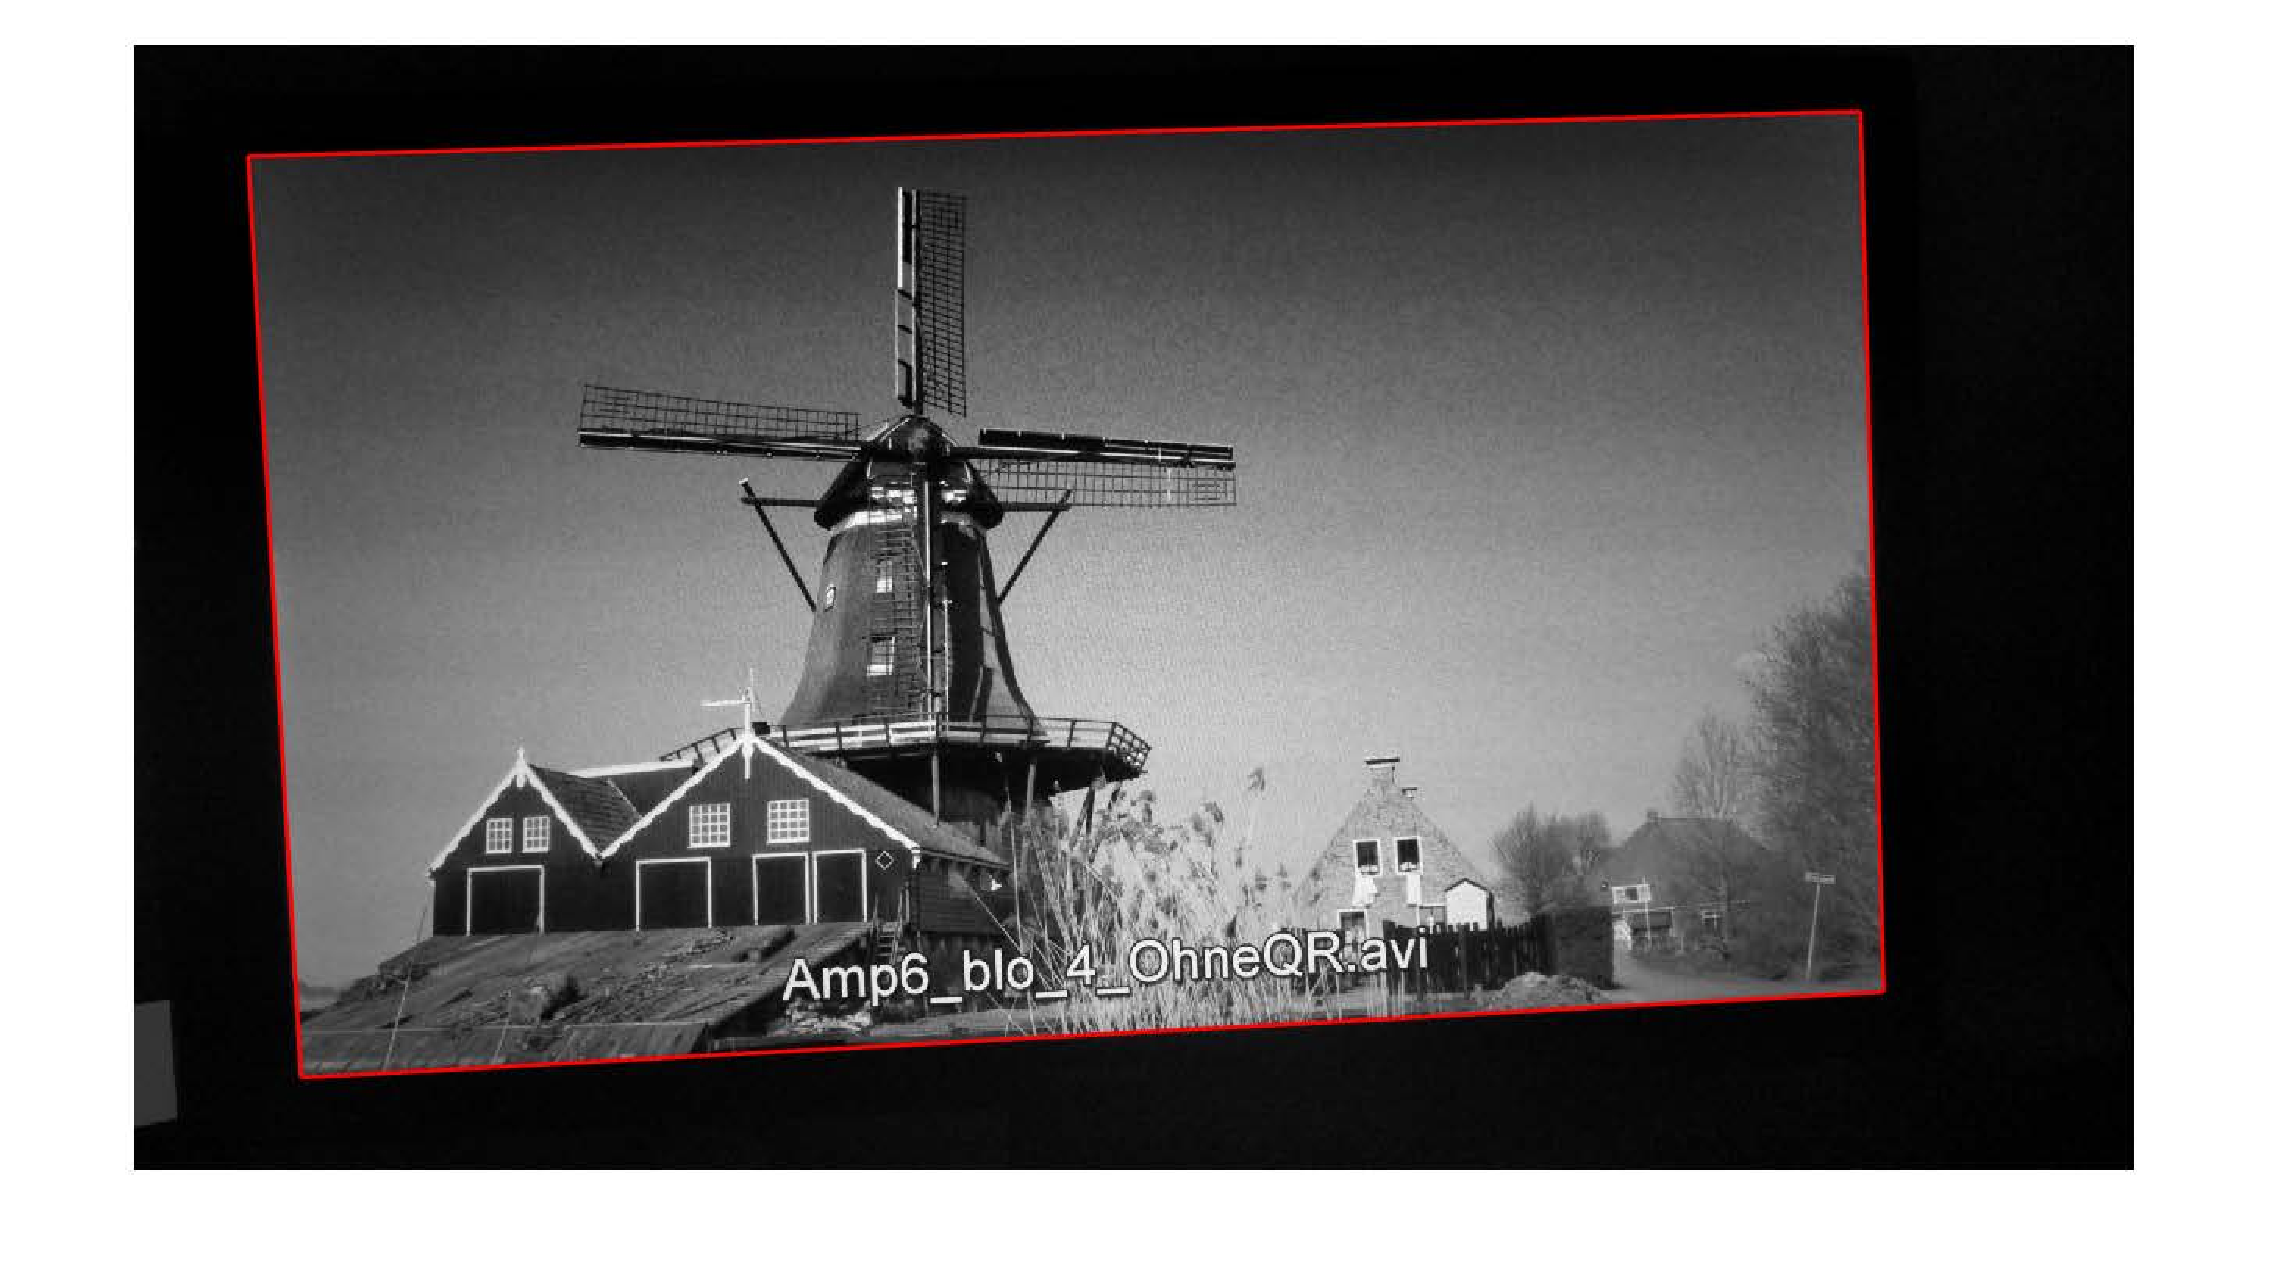
\includegraphics[width=1.0\textwidth]{images/5_Implementirung/2/modulation.pdf}
\caption{Radon Detektion}
\label{fig:radon}
\end{minipage}
\end{figure}

\begin{figure}[H]
 \centering 
  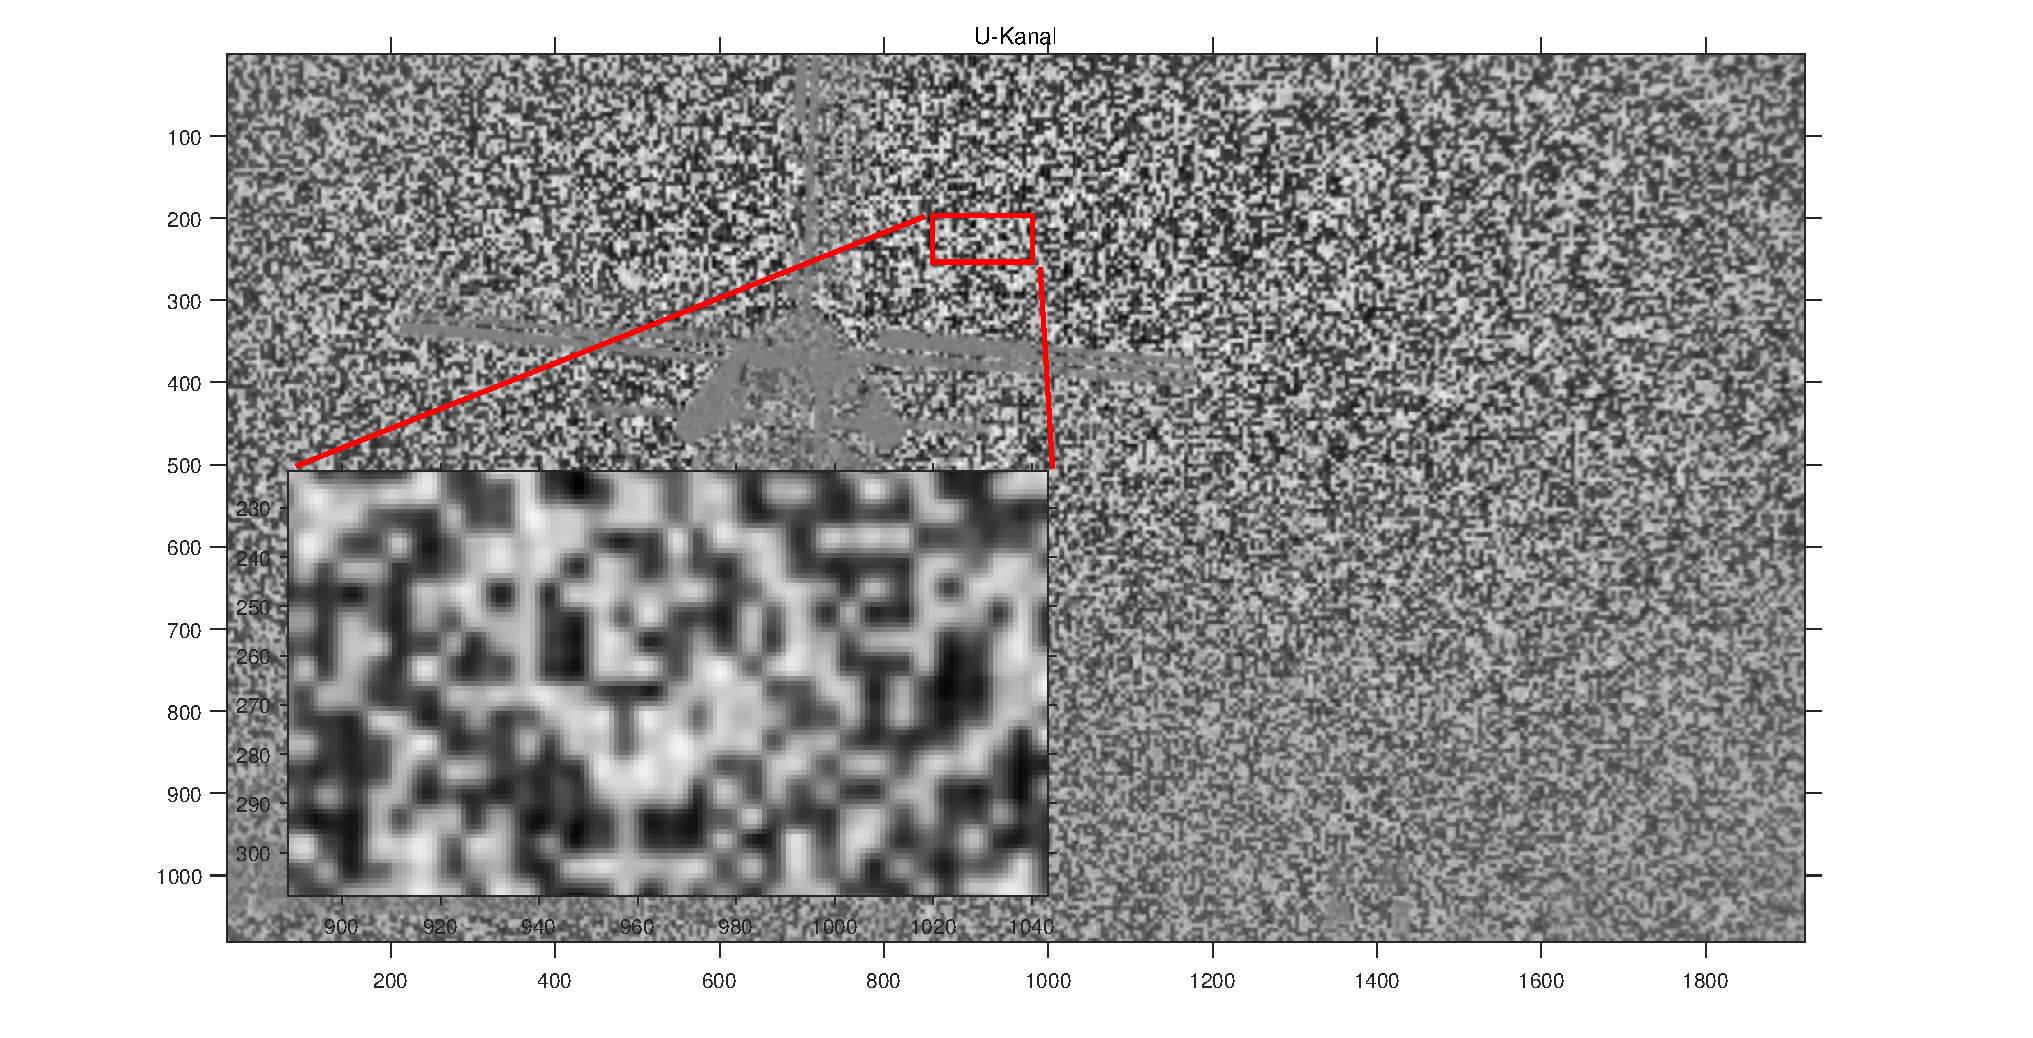
\includegraphics[keepaspectratio,width=1.0\textwidth]{images/5_Implementirung/diff2.eps}
 \caption{Modulationsbereich im U-Kanal}
 \label{fig:Ergebnis1}
\end{figure}



%\begin{figure}[H]
% \centering 
%  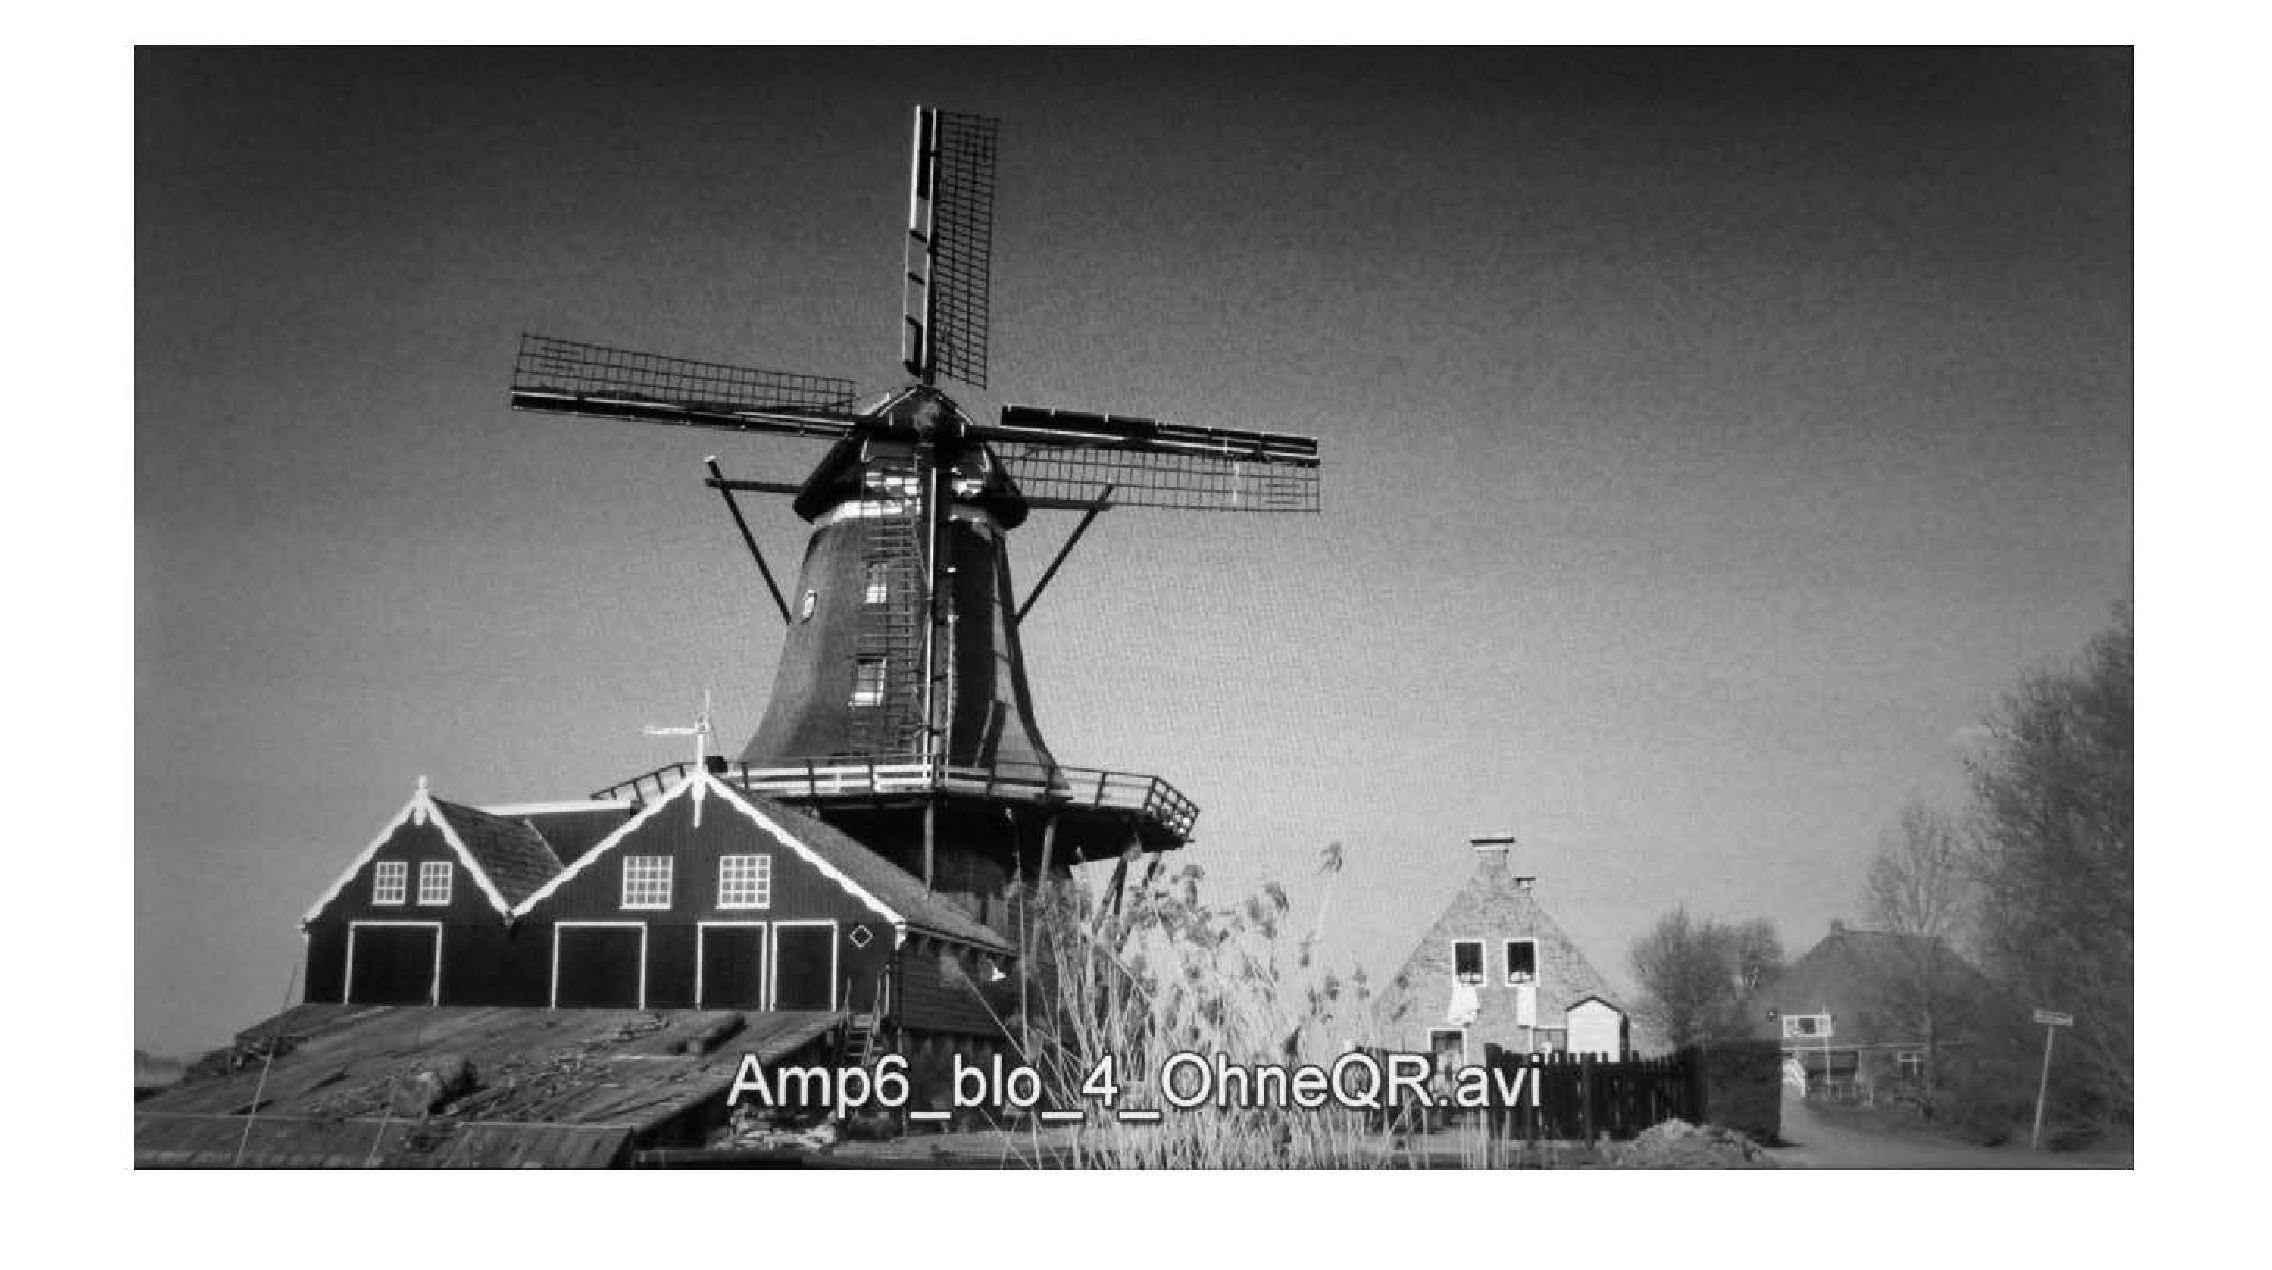
\includegraphics[keepaspectratio,width=1.0\textwidth]{images/5_Implementirung/2/ergebnis.pdf}
% \caption{Ergebnis der 2. Methode}
% \label{fig:Ergebnis1}
%\end{figure}

%Als Nächst einige Ergebnisse der Verwendungen von die 2. Methode wird angegeben.

%Bilder

\section{Implementierung auf einer Smartphone-GPU}

In diesem Abschnitt wird die Implementierung auf einer Smartphone-GPU erläutert. Hier wird Smartphone Xiaomi Mi3 benutzt. Dessen Parameter sind in Tabelle \ref{tbl:Grundlegende Parameter für Mi3} zu sehen. Durch RenderScript als Framework für High Performance Computing auf der Android-Plattform, kann die vorherige Methode auf einer Smartphone-GPU parallel implementiert werden. Die verwendete Software auf der PC-Oberfläche ist Android Studio 3.1.4.

\begin{table}[htb]
	\captionabove{Grundlegende Parameter für Mi3}
	\label{tbl:Grundlegende Parameter für Mi3}
	\footnotesize
	\centering
	\rowcolors{2}{white}{gray!25}	%TUgreen!25
	%\begin{tabular}{|p{2cm}|p{4cm}|p{3cm}|p{3cm}|}	%p{}m{}b{}clr
	\begin{tabular}{|c|c|c|c|}
	\toprule
	\textbf{Smartphone} & \textbf{GPU} & \textbf{CPU} & \textbf{RAM}\\
	\midrule
	Xiaomi Mi3  & Qualcomm Snapdragon 800 MSM8274AB & Krait 400, 2300MHZ & 2 GB, 800 MHZ \\
	\bottomrule
	\end{tabular}
\end{table} 

\textbf{RenderScript}

RenderScript stellt eine native High-Performance-Computing-API bereit, die in C (C99-Standard) geschrieben ist. Mit Renderscript können Anwendungenssoftwares automatisch verschiedene Operationen parallel über alle verfügbaren Prozessorkerne ausführen. Sie bietet auch Unterstützung für verschiedene Verarbeitungsmedien wie CPU, GPU oder DSP. Renderscript ist nützlich für die Grafikverarbeitung, mathematische Modellierung oder jede andere Anwendung die viele mathematische Berechnungen erfordert. Darüber hinaus kann auf all diese Funktionen zugegriffen werden, um verschiedene Architekturen oder eine unterschiedliche Anzahl von Prozessorkernen zu unterstützen ohne Code zu schreiben. Es ist auch nicht notwendig, die Anwendungenssoftware für verschiedene Prozessortypen zu kompilieren, da der RenderSkript-Code kompiliert wird, während er auf dem Gerät ausgeführt wird.

Die Vorteile für RenderScript sind folgende:
\begin{enumerate}
 \item Kompatibilität: Renderscript ist für die Ausführung auf vielen Geräten in verschiedenen Prozessor- (CPU-, GPU- und DSP-Instanzen) Architekturen ausgelegt. Alle unterstützten Architekturen sind nicht für jedes bestimmte Gerät spezifisch, da sein Code zur Laufzeit auf dem Gerät kompiliert und zwischengespeichert wird.
 \item Effizient: Renderscript stellt parallel eine Hochleistungs-Computing-API zur Verfügung, die den Kernel über das gesamte Gerät verteilt.
 \item Einfach zu verwenden: Renderscript vereinfacht die Entwicklung, mit Möglichkeiten wie z.B. das Abbrechen von JNI-Code.
\end{enumerate}

Das Ergebnis der Implementierung auf Xiaomi Mi-3 wird in Abbildung \ref{fig:Ergebnis3} gezeigt.

\begin{figure}[H]
 \centering 
  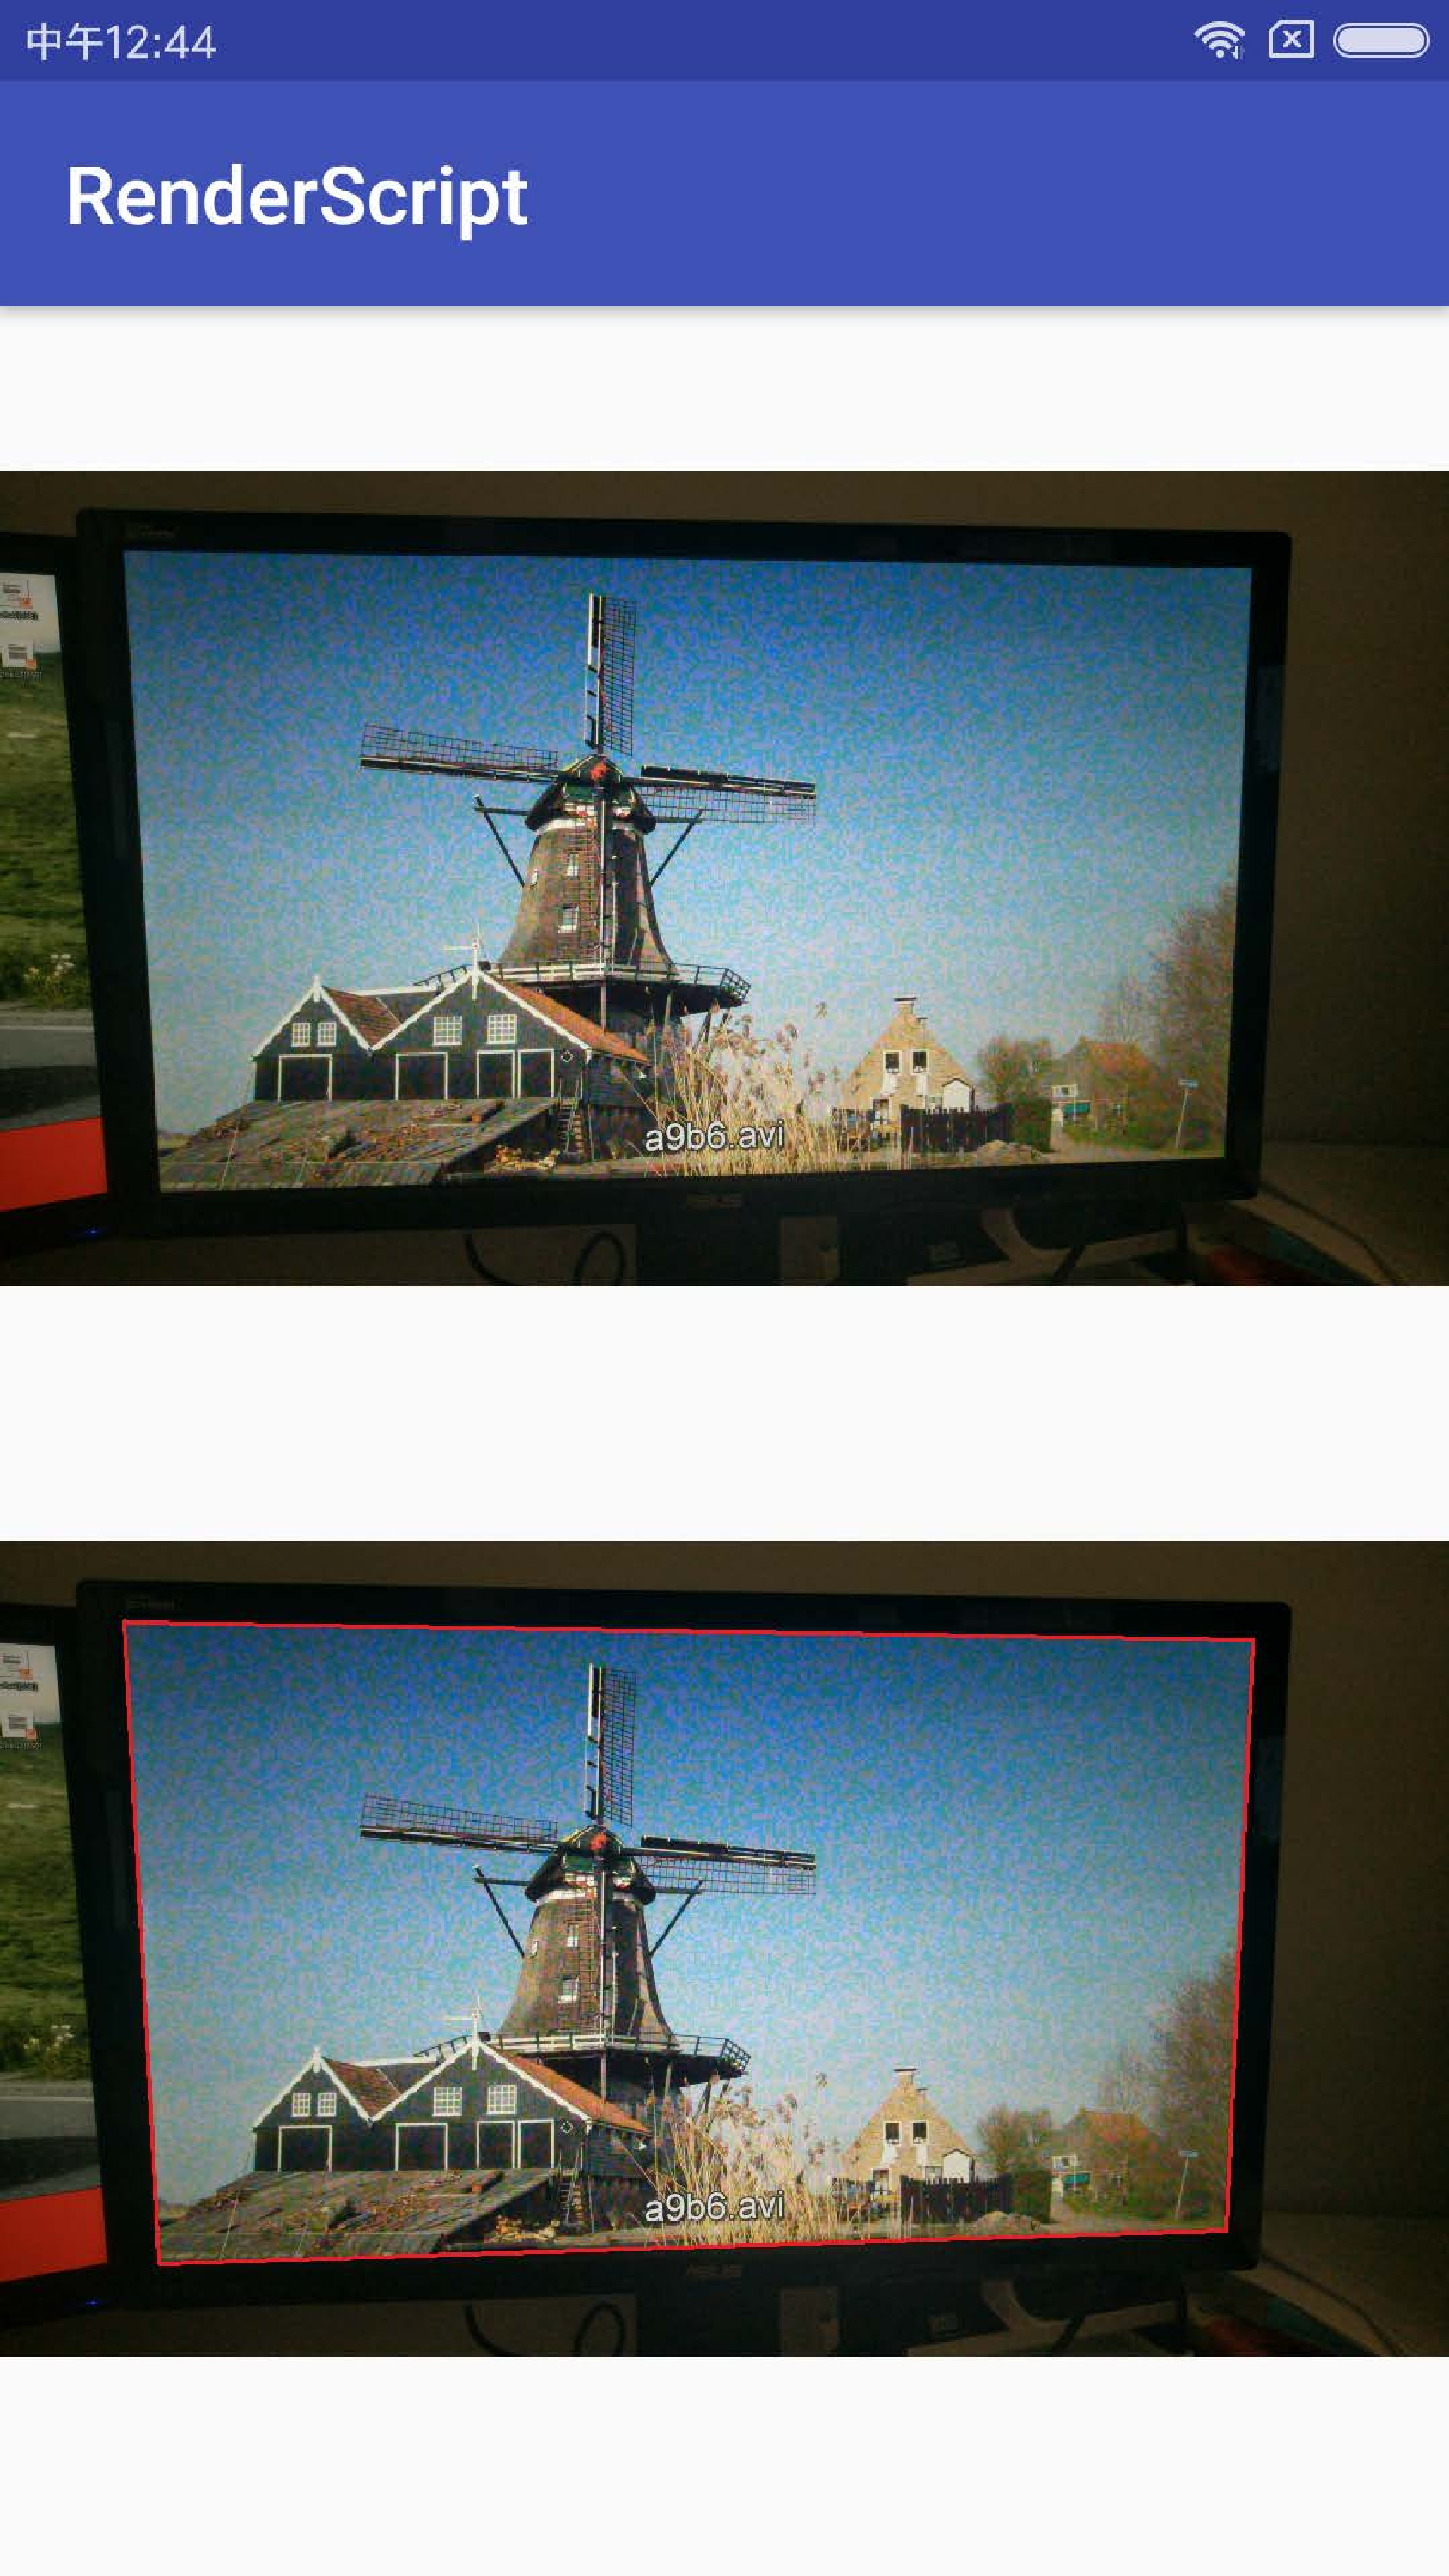
\includegraphics[keepaspectratio,width=0.8\textwidth]{images/5_Implementirung/smartphone.pdf}
 \caption{Ergebnis auf dem Xiaomi Mi3}
 \label{fig:Ergebnis3}
\end{figure}
